\documentclass[10pt]{article}

\usepackage{amsmath}
\usepackage{amssymb}
\usepackage{graphicx}

% ruled/algoruled/plain; lined/vlined/noline
%\usepackage[plain,vlined,noend]{algorithm2e}

%\setlength{\textheight}{9.0in}
%\setlength{\textwidth}{6.50in}
%\setlength{\oddsidemargin}{0.0in}
%\setlength{\topmargin}{-0.5in}

\newcommand{\bincoef}[2]{\left(\!\begin{array}{c}#1\\#2\end{array}\!\right)}

\newcommand{\mycaption}[1]{\caption{\small\it #1}}

\newcounter{gmlrx}
\newcounter{gmlry}
\newcommand{\gmnode}[3]{\put(#1,#2){\circle{20}}\put(#1,#2){\makebox(0,0){$#3$}}}
\newcommand{\gmplate}[5]{
\setcounter{gmlrx}{#1}\addtocounter{gmlrx}{#3}
\setcounter{gmlry}{#2}\addtocounter{gmlry}{-#4}
\put(#1,#2){\line(1,0){#3}}
\put(#1,#2){\line(0,-1){#4}}
\put(\value{gmlrx},\value{gmlry}){\line(-1,0){#3}}
\put(\value{gmlrx},\value{gmlry}){\line(0,1){#4}}
\setcounter{gmlrx}{#1}\addtocounter{gmlrx}{5}
\setcounter{gmlry}{#2}\addtocounter{gmlry}{-6}
\put(\value{gmlrx},\value{gmlry}){\makebox(0,0){$#5$}}
}



\title{Multilevel Bayesian Models \\ of \\ Categorical Data Annotation}

\author{Bob Carpenter
        \\ {\small Alias-i, Inc.}
        \\ {\footnotesize\tt carp@alias-i.com}}

\date{}


\begin{document}
\maketitle

\abstract{\footnotesize
This paper demonstrates the utility of multilevel Bayesian models of
data annotation for classifiers (also known as coding or rating).  The
observable data is the set of categorizations of items by annotators
(also known as raters or coders) from which data may be missing at
random or may be replicated (that is, it handles fixed panel and
varying panel designs).  Estimated model parameters include the
prevalence of category 1 outcomes, the ``true'' category of each item
(the latent class), the accuracy in terms of sensitivity and
specificity of each annotator (latent annotator traits), the
difficulty of each item (latent item traits).  The multilevel
parameters represent the average behavior and variances among the
annotators and the items.  We perform inference with Gibbs sampling,
which approximates the full posterior distribution of parameters as a
set of samples.  Samples from the posterior category distribution may
be used for probabilistic supervision and evaluation of classifiers,
as well as in gold-standard adjudication and active learning.  We
evaluate our approach with simulated data and two real data sets,
including data for which a prior ``gold standard'' exists.}

\section{Introduction}


The goal of this paper is to demonstrate the utility of multilevel
Bayesian approaches to modeling data annotation (also known as coding,
rating, grading, tagging, and labeling).  We focus on categorical data
annotation, as used in training data for classifiers.  Related tasks
such as ranking, rescoring, or sequence tagging may often be reduced
to classification.

Data annotation for classification involves the construction of a
coding standard describing how items should be categorized.  In
practice, several problems invariably arise.  Annotators make mistakes relative
to their own understanding of the coding standard.  Two annotators
might interpret the coding standard differently, each consistently
annotating to a different understanding of the ambiguous standard.  Or
the coding standard might be too vague to determine how a
particular item should be annotated.

We would like to make a range of predictive inferences from the raw
annotations.  Most of all, we would like to infer the correct
categories for items.  We can use these inferences to train and
evaluate classifiers using probabilistic supervision.  Along the way,
it helps to determine if our coding standard is precise enough to
avoid ambiguity and vagueness.  Our models will also allow us to infer
how hard the problem, how variable the annotators are, and how the
items being classified vary in difficulty.  Annotators are not all of
the same ability, and we would like to infer how accurate they are, in
terms of both specificity (true negative rate) and sensitivity (true
positive rate).

The Bayesian models we discuss have the power to jointly reason about
all parameters at all levels.  The multilevel priors help to smooth
individual estimates by combining individual-level data with
group-level data gathered from other individuals (items or
annotators).  We will show that with a simple model of annotation, we
are able to reliably infer the true categories of items and the
underlying accuracy of annotators given only the set of annotations.

The Bayesian nature of our approach allows us to reason about the
uncertainty of each parameter estimated by our model, which is
important for downstream applications such as training and evaluating
classifiers, as well as deciding how to further annotate data or
refine a coding standard in order to arrive at a reliable gold
standard annotation.

We perform all of these inferences with Gibbs sampling, a Bayesian
Markov chain Monte Carlo (MCMC) method.  Gibbs sampling draws
parameter assignments from their posterior distributions.  This allows
general posterior predictive inferences to be made by averaging
results over the samples.

\subsection{Classification}

A classifier assigns categories to input items.  The most widely
studied application of models like ours is in epidemiology, where the
items are people and the raters are diagnostic tests, such as
serological tests (e.g. blood or saliva tests), or diagnostic exams by
medical professionals (e.g. stool tests, x-ray evaluations, physical
exams).  Categories are typically binary (aka dichotomous), being
diseased or non-diseased, but these diagnoses may also be on an
ordinal scale indicating degree of affliction.

Outside of the medical domain, items may be newspaper articles and the
categories the section of the newspaper from which they came.  Or the
input might be a snippet of text and the output the language in which
it is written.  Another example is instances of words in context being
classified as to their part of speech, such as noun or verb, or to
their word sense as defined by a dictionary.  Popular classification
tasks include determining if an e-mail, blog comment, or web page is
spam, whether a discussion of a product is favorable, whether two
mentions of a name or two database records refer to the same person,
whether a word or phrase in one language corresponds to a word or
phrase in another language in a translated text, whether two protein
mentions in a text stand in a regulation relation, whether an
assertion is stated or hedged, whether a text is written from a
conservative, liberal or neutral point of view, \dots.  Sequences of
text characters in a document may be classified as to whether they
refer to a corporation.  From a student's perspective, a true-false or
multiple-choice exam poses a classification problem in which the
questions are the items and the set of answers the categories.

The classification problems we consider require the sets of members of
the categories to be exhaustive and pairwise disjoint.  That is, each
input item must belong to one and only one category.  Topic
identification where zero or more topics may be assigned to each input
may be modeled with a binary classifier per topic.

We will focus on binary classification problems (also known as
dichotomous classification), in which there are only two categories,
which we will code as 0 and 1.  Document search on the web may be
modeled as a binary classification problem with items consisting of
pairings of a search query and a document, with category 1 assigned to
if the document is relevant to the query, and 0 assigned otherwise.

A more general problem involves regression of ordinal outputs, such as
assessing customer satisfication from a survey employing a Likert
scale, or rating restaurants on a $\{0,1,2,3\}$ star scale.  At some
point, it makes sense to consider continuous scales, as in rating
wines from 0--100 on some scale, or rating gymnasts from 0--10 on
execution and from 0--10 on difficulty.  We do not explore these
generalizations in this paper.


\subsection{Coding Standards}

A classification task requires a coding standard which defines how
items are to be categorized.  A coding standard may be nothing more
than shared knowledge among a group of annotators.  A coding standard
typically includes example instances and their corresponding
categories.  More formal coding standards include written guidelines
attempting to specify which items should be assigned to which
categories.

Coding standards are constructed by one or more developers.  For
instance, the set of part of speech tags for a language is not known,
but is instead developed by one or more linguists.  Similarly, the set
of ICD-9 diagnosis codes is developed by doctors and insurers.  The
grades of a French vineyard are defined by a communal process.  In all
of these cases, the coding standard is likely to evolve over time.

For instance, most United States-based insurers require patients to be
categorized using the International Classification of Diseases, 9th
Revision, Clinical Modification (ICD-9-CM).  The U.~S.~Federal
Government's guidelines for ICD-9 coding runs to 71 pages, with
contents like

\begin{quote}
\noindent
If the type of diabetes mellitus is not documented in
the medical record the default is type II.
\\
\mbox{ }
\hfill
(CMMS and DHSS, 2005;
guideline 3.1.2, p.~21)
\end{quote}

The Penn Treebank part-of-speech tagging guidelines
includes rules such as:

\begin{quotation}
\noindent
Abbreviations and initials should be tagged as if they were spelled
out.  Thus, {\it S\&L} (which stands for {\it savings and loan}) should
be tagged as a common noun (NN), not as a proper noun (NP). By
contrast, {\it the U.~S.}~should be tagged as {\it the~U.~S./NP}.
\\
\mbox{ }
\hfill (Santorini 1990, p.~18)
\end{quotation}

With any coding standard, the question arises as to whether it is well
enough specified that it can be applied consistently by annotators.
This is the inter-annotator agreement problem (equivalently
inter-rater agreement or inter-coder agreement problem).


\subsection{Bayesian Inference}

Bayesian inference involves creating a complete probability model over
all data and parameters of interest, fitting the model to observed
data, then reasoning about either the fitted parameters or about new
data taking into account the uncertainty in the fitted parameters.

Bayesian inference is powerful enough to estimate group level effects,
such as problem difficulty, as well as individual effects, such as
annotator accuracy.  Bayesian inference is still effective when data
is missing, which amounts to annotators not annotating every example.

In practice, a Bayesian model is specified by a prior and a
likelihood/data sampling function.  The data sampling or likelihood
function $p(x|\theta)$ defines the probability of the data $x$ given
the model parameters $\theta$ (it is called the sampling function if
$\theta$ is fixed and the likelihood function if $x$ is fixed).  The
prior $p(\theta)$ defines the prior likelihood of the parameters
$\theta$ before we have seen any data.  The posterior distribution
$p(\theta|x)$ over the parameters $\theta$ given data $x$ is
calculated by first applying Bayes's rule and then computing the
marginal data probability $p(x)$ by averaging the conditional data
distribution $p(x|\theta)$ over the prior parameter distribution
$p(\theta)$.
%
\begin{equation}\label{bayes-post.eq}%
p(\theta|x)
= \frac{p(x|\theta) p(\theta)}
       {p(x)}
%
= \frac{p(x|\theta) p(\theta)}
       {\int p(x|\theta) p(\theta) d\theta}
%
\propto p(x|\theta) p(\theta)
\end{equation}
%

Predictive inference for new data $y$ given observed training data $x$
is performed by averaging the conditional data distribution
$p(y|\theta)$ over the posterior parameter distribution $p(\theta|x)$, setting
\[
p(y|x) = \int p(y|\theta) p(\theta|x) d\theta
\]
where the integral is over the valid range of the parameters $\theta$.

A uniform prior $p(\theta)$ is noninformative in the sense that it
drops out of the equation for the posterior, reducing
equation~(\ref{bayes-post.eq}) to $p(\theta|x) \propto p(x|\theta)$.  With a
noninformative prior, the posterior $p(\theta|x)$ for the parameters
is fully determined by the likelihood function $p(x|\theta)$.

A family of distributions $\mathcal{F}$ is said to be a conjugate prior
for a family of distributions $\mathcal{G}$ if for any prior
distribution $p(\theta) \in
\mathcal{F}$ and likelihood function $p(x|\theta) \in \mathcal{G}$, the
posterior distribution $p(\theta|x) \in \mathcal{F}$.

In this paper, Bayesian inference will be carried out by computer
simulation.  The simulations employ Markov chain Monte Carlo (MCMC)
methods.  These Markov chains are constructed directly using
conditional sampling wherein each parameter is sampled given the
previous values of all other samples.  A complete sample of all
parameters constitutes a state of the Markov chain.  The stationary
distribution of states in the chain simulates the posterior
distribution over parameters.  We summarize simulated estimates with
statistics over the samples, such as means, percentiles such as
medians which may be used to construct posterior intervals.  In all
cases, several chains are used to assess convergence, and a fixed
initial segment of samples is discarded.

\section{Models}

In this section, we'll outline an increasingly rich set of models of
the annotation process.  All of our models are latent class models in
the sense that they estimate the unknown true category of each item.

We begin with a binomial model that assumes sensitivity and
specificity do not vary across annotators or items.  This will allow
us to introduce notation in a simple setting.

We extend the simple model to a multilevel model in two ways.
First, we introduce a beta-binomial model in which sensitivity and
specificity vary by annotator, but all items are treated as equally
difficult.  A common beta prior models the mean and variance of
annotator sensitivity and specificities.  These are sometimes called
latent traits of the annotator.

We next consider a complementary beta-binomial model in which all
annotators are equally accurate, but items vary by difficulty.  In
this model, we have beta priors for category 0 and category 1 problems
that model the distribution of difficulties of items of those
categories.  These parameters represent latent traits of the items.

Finally, we introduce a non-nested multilevel generalized linear model
in which annotators may vary in sensitivity and specificity and where
items may vary in difficulty.  This has been called a general latent
trait model, or in the regression literature, a random effects model.
With more information about items or annotators, this model can be
easily extended to other item-level or annotator-level predictors.
With more information about item- and annotator grouping, it can also
be extended to group-level predictors.  We do not consider these
extensions here.

All four of these models account for data missing at random, which in
this case amounts to not having every annotator label every item.
This corresponds to a varying panel design, which generalizes the
standard fixed panel design in which every item is labeled by every
annotator.  They are also able to handle replicated data, which
involves having the same annotator annotate the same item more than
once (though the models assume these annotations are independent given
the item).

Parameter estimates are not biased as long as the missingness does not
depend on features of the item or the annotator.  It is common for
there to be a large number of items and annotators, with every item
being labeled by a random subset of annotators.

We will evaluate Bayesian inference for these models with simulated
data in the next section and real data in the following section.



\subsection{Binomial Model}


\begin{figure}
\begin{center}
\begin{picture}(195,120)

\gmnode{77.5}{92.5}{\theta_{0}}
\gmnode{162.5}{92.5}{\theta_{1}}
\gmnode{10}{30}{\pi}
\gmnode{55}{30}{c_i}
\gmnode{120}{30}{x_k}

\put(20,30){\vector(1,0){25}}  % \pi to c_i
\put(65,30){\vector(1,0){45}}  % c_i to x_k
\put(77.5,82.5){\vector(1,-1){42.5}}  % theta_0_j to x_k
\put(162.5,82.5){\vector(-1,-1){42.5}}  % theta_1_j to x_k

\gmplate{30}{55}{50}{50}{I}
\gmplate{95}{55}{50}{50}{K}

\end{picture}
%
\begin{eqnarray*}
c_i & \sim & \mathsf{Bernoulli}(\pi)
\\
x_{k} & \sim & \mathsf{Bernoulli}(c_{ii_k} \theta_{1}
                                       + (1 - c_{ii_k}) (1 - \theta_{0}))
\\[8pt]
\pi & \sim & \mathsf{Beta}(1,1)
\\
\theta_{0} & \sim & \mathsf{Beta}(1,1)
\\
\theta_{1} & \sim & \mathsf{Beta}(1,1)
\end{eqnarray*}
\end{center}
\mycaption{Binomial Model}\label{binomial-model.fig}
\end{figure}

The binomial model is presented in Figure~\ref{binomial-model.fig}. As with
all of our models, we present the standard sketch of a graphical model
using node/plate notation and more fully using sampling notation.
This is the same notation as is used to implement models in BUGS.

The graphical model notation in Figure~\ref{binomial-model.fig} represents
the random variables of the model as nodes in the graph.  For
instance, the variable $\pi$ represents the prevalence of the category
1 among items.  In our graphs, we have supressed constant
hyperparameters representing noninformative priors; these are often
represented as square nodes.  The edges of the graph represent
dependencies between random variables.  Finally, the rectangular
plates represent multiple versions of the same variable, with
the size of the replicate set indicated in the upper-left corner.
For example, there are $I$ variables $c_1, \ldots, c_I$ representing
the categories of items.  Each item category variable $c_i$ is
conditioned on the prevalence variable $\pi$.

The sampling notation makes the conditional dependencies explicit along
with the noninformative priors left out of the graphical sketch.  The
notation $\pi \sim \mathsf{Beta}(1,1)$ indicates that the variable $\pi$ is
drawn from a beta distribution with parameters (1,1), which, as we'll see,
is just a convenient way to write a uniform distribution over the interval
[0,1].

In general, a beta distribution has parameters $\alpha$ and $\beta$,
with a probability density defined for $x \in [0,1]$ by:
\[
\mathsf{Beta}(x|\alpha,\beta) \propto x^{\alpha - 1} (1 - x)^{\beta - 1}
\]
With $\alpha = \beta = 1$, the beta reduces to a uniform distribution:
\[
\mathsf{Beta}(x|1,1)
\propto x^{(1-1)} (1-x)^{(1-1)}
= 1
= \mathsf{Uniform}(x|0,1)
\]

The (bounded) uniform distribution has a constant density over a
finite interval $(\delta,\gamma)$, $\delta < \gamma$:
\[
\mathsf{Uniform}(x|\delta,\gamma)
=\
\left\{
\begin{array}{ll}
\frac{1}{\gamma - \delta} & \mbox{ if } \delta \leq x \leq \gamma
\\[4pt]
0 & \mbox{ otherwise}
\end{array}
\right.
\]

The parameters $\theta_0$ and $\theta_1$ representing specificity
and sensitivity are also drawn from uniform $\mathsf{Beta}(1,1)$ distributions.
Then, for each item $i$, $c_i$ is drawn from $\mathsf{Bernoulli}(\pi)$.

The Bernoulli is a discrete distribution with two outcomes, $\{ 0, 1
\}$, which may be described as binary, boolean or dichotomous.
There is a single parameter $\theta$ representing the likelihood of a 1
outcome:
\[
\mathsf{Bernoulli}(c|\theta)
=
\left\{
\begin{array}{ll}
\theta & \mbox{ if } c = 1
\\[4pt]
(1 - \theta) & \mbox{ if } c = 0
\end{array}
\right.
\]

To deal with missing and/or replicated data, we use a notation where
there are $K$ annotations $x_1,\ldots,x_k$, where item $x_k$ is the
label by annotator $jj_k$ of item $ii_k$.  The variables $ii$ and $jj$
are index vectors of length $K$ taking values in $1,\ldots,I$ and
$1,\ldots,J$ respectively.  This representation is general enough to
accomodate a fixed panel design where every annotator labels every
item, and also any variation of variable panel design where an
annotator may label an item zero, one or more times.

The complexity in notation for sampling $x_k$ is because we have
independently parameterized specificity and sensitivity.  If the true
category $c_{ii_k} = 0$, the likelihood of an annotator assigning the
correct label is $\theta_0$.  If the true category $c_{ii_k} = 1$, the
likelihood of an annotator assigning the correct label is $\theta_1$.
The arithmetic is to convert the accuracy and true label into an
appropriate Bernoulli parameter.  If $c_{ii_k} = 1$, the expression
inside the Bernoulli for $x_k$ reduces to $\theta_1$, meaning $P(x_k =
1) = \theta_1$.  If $c_{ii_k} = 0$, the expression reduces to
$1-\theta_0$, meaning $P(x_k = 1) = 1-\theta_0$, or $P(x_k = 0) =
\theta_0$.

The joint probability for all of the data and parameters is:
\[
\begin{array}{l}
p(\pi,c,\theta_0,\theta_1,x)
\\[4pt]
\ \ \ = p(\pi) p(\theta_0) p(\theta_1) \prod_i p(c_i | \pi) \prod_k p(x_k|\theta_0,\theta_1,c)
\\[4pt]
\ \ \ = \mathsf{Beta}(\pi|1,1) \mathsf{Beta}(\theta_0|1,1) \mathsf{Beta}(\theta_1|1,1)
\\ \ \ \ \ \ \ \ \
\prod_i \mathsf{Bernoulli}(c_i|\pi) \prod_k \mathsf{Bernoulli}(x_k | c_{ii_k}\theta_1 + (1 - c_{ii_k})(1 - \theta_0))
\\[4pt]
\ \ \ = \prod_i \mathsf{Bernoulli}(c_i|\pi) \prod_k \mathsf{Bernoulli}(x_k | c_{ii_k}\theta_1 + (1 - c_{ii_k})(1 - \theta_0))
\end{array}
\]
With the annotations and indices supplied as data, the estimate we
supply is of the posterior distribution $p(\pi,c,\theta_0,\theta_1|x)$
over parameters given the data.  The Gibbs sampler simulates draws of
the complete parameter vector $(\pi,c,\theta_0,\theta_1)$ from the
posterior distribution.

\subsection{Identifiability} 

As stated, the model has a symmetric bimodal likelihood space.  For
every parameter assignment $(c,\pi,\theta_0,\theta_1)$, there is an
equally likely parameter assignment
$(1-c,1-\pi,1-\theta_1,1-\theta_0)$, where every assignment in $c$ is
reversed, $c'_i = 1 - c_i$, where the prevalence is reflected around
0.5, and the sensitivity and specificity parameters are swapped and
reflected around 0.5.  For instance, suppose we have a prevalence of
$\pi$, specificity $\theta_0$, sensitivity $\theta_1$, and an item
annotated by three annotators with annotations $1$, $1$, and $0$, with
category assignment 1.  The likelihood contributed by the item and
annotations is $\pi \theta_1 \theta_1 (1 - \theta_1)$.  If we take $\pi' = 1 - \pi$, $\theta_0' = 1-\theta_1$, $\theta_1' = 1 - \theta_0$, and
consider the same annotation data $110$, only this time with category
assignment 0, the likliehood is $(1 - \pi') (1 - \theta_0') (1 -
\theta_0') \theta'_0 = \pi \theta_1 \theta_1 (1 - \theta_1)$.

There are three ways to get around this non-identifiability in
practice.  First, the priors could be made strong and asymmetric over
the $\theta$ parameters to favor one solution over the other.  Second,
the values for $\theta$ parameters can be restricted to be greater
than 0.5, which is what we did in fitting (some of) the models.  This
is less desirable in general in that some values fitted in real data
sets have sensitivities less than 0.5.  Third, the Markov chains in
the Gibbs sampler could be allowed to find either result, then it can
be converted to a canonical representation using the transform
presented above.  

We chose the second approach for expediency in the simple binomial
model.  As is often the case, in our more complex models, the
non-identifiability is mitigated in practice by choosing reasonable
initial values, which leads the Gibbs sampler to investigate the area
around only one mode of the likelihood space.

Inferences for new annotations $y$ are carried out in the usual
Bayesian fashion by integrating out the parameter estimates by
treating them as a mixture weighted by estimated posterior likelihood:
\[
p(y|x) = \sum_{c \in \{ 0, 1\}^I} \int_0^1 \int_0^1 \int_0^1 p(y|c,\pi,\theta_0,\theta_1) p(\pi,\theta_0,\theta_1,c|x) d\pi d\theta_0 d\theta_1
\]
For inference about relabeling existing data, the sum over the vector
of Bernoulli variables $c_i$ may be removed, whereas inference about
getting another labeler to annotate an existing item $i$ requires the
estimate of $c_i$.  The Gibbs samples allow a simulation-based
evaluation of the integral required for posterior inference.  With
$N$ samples,
\[
(c^{(1)}, \pi^{(1)}, \theta_0^{(1)}, \theta_1^{(1)}),
\ldots, (c^{(N)}, \pi^{(N)}, \theta_0^{(N)}, \theta_1^{(N)})
\] 
we approximate posterior inference to
an arbitrary level of precision with
\[
p(y|x) \approx \frac{1}{N}  \sum_{1 \leq n \leq N} p(y|c^{(n)}, \pi^{(n)}, \theta_0^{(n)}, \theta_1^{(n)})
\]
The use of the approximation is justified by the limit:
\[
p(y|x) = \lim_{N \rightarrow \infty} \sum_{1 \leq n \leq N} p(y|c^{(n)}, \pi^{(n)}, \theta_0^{(n)}, \theta_1^{(n)})
\]

Marginal posterior distributions for individual variables or arbitrary
subsets of variables are simply approximated by restricting the
samples to one or more variables.  This allows summary statistics such as
posterior means and intervals to be calculated on the samples.  For
instance, the posterior estimate for mean prevalence $\pi$ is
approximated by the mean of $\pi^{(1)},\ldots,\pi^{(N)}$, whereas the
posterior 95\% interval is calculated using the 2.5\% and 97.5\%
quantiles of the sample $\pi^{(1)},\ldots,\pi^{(N)}$.

Given the true category of an item, the distribution of true positives
and the distribution of true negatives follow binomial distributions
with success parameters $\theta_1$ and $\theta_0$ respectively.  To
make this precise, define the number of true and false items by:
\[
T = \sum_k c_{ii_k}
\ \ \ \ \ \ \ \ 
F = \sum_k (1 - c_{ii_k})
\]
The number of true-positive and true negative annotations are
given by:
\[
\mbox{\it TP} = \sum_k c_{ii_k} a_k
\ \ \ \ \ \ \ 
\mbox{\it TN} = \sum_k (1 - c_{ii_k}) (1 - a_k)
\]
With the simple binomial model, the true positives and true
negatives are distributed as binomials:
\[
\mbox{\it TP} \sim \mathsf{Binomial}(\theta_1,T)
\ \ \ \ \ \ \ 
\mbox{\it TN} \sim \mathsf{Binomial}(\theta_0,F)
\]

A binomial distribution $\mathsf{Binomial}(\theta,n)$ assigns non-zero
probability to integer outcomes $0, \ldots, n$ based on the likelihood
of that many successes out of $n$ independent Bernoulli trials with
parameter $\theta$.  The distribution is:
\[
\mathsf{Binomial}(k|\theta,n)
= \binom{n}{k} \theta^k (1-\theta)^{n-k}
\]
With the number of trials $n$ fixed by design, the binomial
distribution has only a single parameter $\theta$ which determines
both the mean and variance of the distribution, which are
$n\theta$ and $n\theta(1-\theta)$ respectively.

We can factor true positives and false positives by annotator, with
the true positives for annotator $j$ defined by
\[
\mbox{\it TP}_{j} = \sum_k \mathrm{I}(jj_k = j) c_{ii_k} x_k
\]
where the indicator funtion $\mathrm{I}(\phi)$ is defined to be 1
if the condition $\phi$ is true and 0 otherwise.  True negatives
$\mbox{\it TN}_{j}$ for annotator $j$ are defined similarly, as
\[
\mbox{\it TN}_{j} = \sum_k \mathrm{I}(jj_k = j) (1 - c_{ii_k}) (1 - x_k)
\]
The number of true and false items also varies by annotator and by
item, with
\[
\mbox{\it T}_{j} = \sum_k \mathrm{I}(jj_k = j) c_{ii_k}
\ \ \ \ \ \ \ 
\mbox{\it F}_{j} = \sum_k \mathrm{I}(jj_k = j) (1 - c_{ii_k})
\]
The simple binomial model assumes an identical chance of success for
each annotator, so that
\[
\mbox{\it TP}_{j} \sim \mathsf{Binomial}(\theta_1,\mbox{\it T}_{j})
\ \ \ \ \ \ \ 
\mbox{\it TN}_{j} \sim \mathsf{Binomial}(\theta_0,\mbox{\it F}_{j})
\]

We can also factor by item.  For item $i$, the total number of annotations
is
\[
L_i = \sum_k I(ii_k = i)
\]
with the number of positive and negative annotations
\[
\mbox{\it P}_i = \sum_k \mathrm{I}(ii_k = i) x_k
\]
\[
\mbox{\it N}_i = \sum_k \mathrm{I}(ii_k = i) (1 - x_k) = L_i - P_i
\]
The distribution of positive or negative annotations is
binomial in the relevant parameter.  For positive cases, $c_i=1$,
and negative cases, $c_i = 0$, we have:
\[
\mbox{\it P}_i \sim \mathsf{Binomial}(\theta_1,L_i)
\ \ \ \ \ \ \
\mbox{\it N}_i = \sim \mathsf{Binomial}(\theta_0,L_i)
\]

This model and all subsequent models provide an estimate of the
posterior distribution of the item categories $c$.  This estimate is
based on the Gibbs sampler, which in turn is based on a conditional
estimate of $c$ given the other model parameters.  The estimate of $c$
is straightforward given the inferred binomial parameters $\theta$,
the inferred prevalence parameter $\pi$, and the observed annotations
$a$.

The inferred item categories may be used to compute posterior
statistics such as prevalence (not to be confused with the prevalence
parameter $\pi$), and annotator sensitivity and specificity (not to be
confused with the binomial parameters $\theta_0$ and $\theta_1$).
Although all models fit $\pi$ to be close to the prevalence, in the
binomial and beta-binomial by item models, all annotators are fit with
the same sensitivity and specificity parameter, so they won't be a
particularly good fit to any annotator in general.  In the
beta-binomial by annotator and logistic models, which do estimate a
per-annotator sensitivity and specificity parameter, the estimates
will be affected by the priors, which will move the posterior
estimates away from the maximum likelihood solution and toward the
prior.  The point of pooling with priors is that the estimates should
be a better predictor of future specificity and sensitivity.


\subsection{Beta-Binomial by Annotator}

The simple binomial model is underdispersed in that the counts
$\mbox{\it TP}_j$ and $\mbox{\it TN}_j$ have a larger sample variance
than can be represented with a binomial distribution.  The model in
Figure~\ref{beta-binomial-anno-model.fig} allows the specificity and
sensitivity parameters to vary by annotator, amounting to
a beta-binomial distribution of the true positives and true negatives
by annotator.

\begin{figure}
\begin{center}
\begin{picture}(195,145)

\gmnode{57.5}{132.5}{\alpha_0}
\gmnode{97.5}{132.5}{\beta_0}
\gmnode{142.5}{132.5}{\alpha_1}
\gmnode{182.5}{132.5}{\beta_1}
\gmnode{77.5}{92.5}{\theta_{0,j}}
\gmnode{162.5}{92.5}{\theta_{1,j}}
\gmnode{10}{30}{\pi}
\gmnode{55}{30}{c_i}
\gmnode{120}{30}{x_k}

\put(57.5,122.5){\vector(1,-1){19.75}}  % alpha_0 to theta_0_j
\put(97.5,122.5){\vector(-1,-1){19.75}} % beta_0 to theta_0_j
\put(142.5,122.5){\vector(1,-1){19.75}}  % alpha_1 to theta_1_j
\put(182.5,122.5){\vector(-1,-1){19.75}} % beta_1 to theta_1_j
\put(20,30){\vector(1,0){25}}  % \pi to c_i
\put(65,30){\vector(1,0){45}}  % c_i to x_k
\put(77.5,82.5){\vector(1,-1){42.5}}  % theta_0_j to x_k
\put(162.5,82.5){\vector(-1,-1){42.5}}  % theta_1_j to x_k

\gmplate{30}{55}{50}{50}{I}
\gmplate{95}{55}{50}{50}{K}
\gmplate{45}{115}{150}{45}{J}

\end{picture}
%
\begin{eqnarray*}
c_i & \sim & \mathsf{Bernoulli}(\pi)
\\
\theta_{0,j} & \sim & \mathsf{Beta}(\alpha_0,\beta_0)
\\
\theta_{1,j} & \sim & \mathsf{Beta}(\alpha_1,\beta_1)
\\
x_k & \sim & \mathsf{Bernoulli}(c_{ii_k} \theta_{1,jj_k}
                                + (1 - c_{ii_k}) (1 - \theta_{0,jj_k}))
\\[8pt]
\pi & \sim & \mathsf{Beta}(1,1)
\\
\alpha_0/(\alpha_0 + \beta_0) & \sim & \mathsf{Beta}(1,1)
\\
\alpha_0 + \beta_0 & \sim & \mathsf{Pareto}(1.5)
\\
\alpha_1/(\alpha_1 + \beta_1) & \sim & \mathsf{Beta}(1,1)
\\
\alpha_1 + \beta_1 & \sim & \mathsf{Pareto}(1.5)
\end{eqnarray*}
\end{center}
\mycaption{Beta-Binomial by Annotator Model}\label{beta-binomial-anno-model.fig}
\end{figure}

Now for each annotator $j$, a specificity $\theta_{0,j}$ and a
sensitivity $\theta_{1,j}$ are sampled from beta priors with
parameters $(\alpha_0,\beta_0)$ and $(\alpha_1,\beta_1)$ respectively.
The parameters are part of the model and thus themselves have priors.
For specifying priors, we reparameterize the beta distribution
$\mathsf{Beta}(\alpha,\beta)$ in terms of mean $\alpha / (\alpha +
\beta)$ and scale $\alpha + \beta$.  We put a uniform prior on the
mean and a uniform prior on the inverse square scale
$1/(\alpha+\beta)^2$.  The uniform prior on the means are expressed
using a $\mathsf{Beta}(1,1)$ prior for convenience.  The uniform prior
on the inverse square scale works out to a Pareto prior
$\mathsf{Pareto}(1.5)$ on the scale $\alpha + \beta$.  The Pareto
distribution is a power-law distribution defined by:
\[
\mathsf{Pareto}(x|\theta) \propto x^{-(\theta+1)}
\]

The joint probability distribution for all parameters works out to:
\[
\begin{array}{l}
p(\alpha_0,\beta_0,\alpha_1,\beta_1,\pi,\theta_0,\theta_1,\pi,c,x)
\\[8pt]
\ \ \ = p(\alpha_0,\beta_0) p(\alpha_1,\beta_1) p(\pi)
\\[2pt]
\ \ \ \ \ \ \ \
\prod_j p(\theta_{0,j}|\alpha_0,\beta_0) p(\theta_{1,j}|\alpha_1,\beta_1)
\\[2pt]
\ \ \ \ \ \ \ \
\prod_i p(c_i|\pi)
\\[2pt]
\ \ \ \ \ \ \ \
\prod_k p(x_k|c,\theta_0,\theta_1)
\\[8pt]
\ \ \ =
\mathsf{Beta}(\alpha_0/(\alpha_0+\beta_0)|1,1) \mathsf{Pareto}(\alpha_0 + \beta_0|1.5)
\\[2pt]
\ \ \ \ \ \ \ \
\mathsf{Beta}(\alpha_1/(\alpha_1+\beta_1)|1,1) \mathsf{Pareto}(\alpha_1 + \beta_1|1.5)
\mathsf{Beta}(\pi|1,1)
\\[2pt]
\ \ \ \ \ \ \ \
\prod_i \mathsf{Bernoulli}(c_i|\pi)
\\[2pt]
\ \ \ \ \ \ \ \
\prod_j \mathsf{Beta}(\theta_{0,j}|\alpha_0,\beta_0) \mathsf{Beta}(\theta_{1,j}|\alpha_1,\beta_1)
\\[2pt]
\ \ \ \ \ \ \ \
\prod_k \mathsf{Bernoulli}(x_k|c_{ii_k}\theta_{1,jj_k} + (1-c_{ii_k})(1-\theta_{0,jj_k}))
\\[8pt]
\ \ \ =
\mathsf{Pareto}(\alpha_0 + \beta_0|1.5)
\mathsf{Pareto}(\alpha_1 + \beta_1|1.5)
\\[2pt]
\ \ \ \ \ \ \ \
\prod_i \mathsf{Bernoulli}(c_i|\pi)
\\[2pt]
\ \ \ \ \ \ \ \
\prod_j \mathsf{Beta}(\theta_{0,j}|\alpha_0,\beta_0) \mathsf{Beta}(\theta_{1,j}|\alpha_1,\beta_1)
\\[2pt]
\ \ \ \ \ \ \ \
\prod_k \mathsf{Bernoulli}(x_k|c_{ii_k}\theta_{1,jj_k} + (1-c_{ii_k})(1-\theta_{0,jj_k}))
\end{array}
\]

The true positives and true negatives per-annotator are distributed
beta-binomial in this model with parameters $(\alpha_1,\beta_1)$ and
$(\alpha_0,\beta_0)$ respectively:
\[
\mbox{\it TP}_j \sim \mbox{\sf Beta-Binomial}(\alpha_1,\beta_1,P_j)
\]
\[
\mbox{\it TN}_j \sim \mbox{\sf Beta-Binomial}(\alpha_0,\beta_0,N_j)
\]

The beta-binomial is an infinite mixture model, mixing binomials
with respect to their beta likelihood:
\[
\mbox{\sf Beta-Binomial}(k|\alpha,\beta,n)
= \int_0^1 \mbox{\sf Binomial}(k|\theta) \mbox{\sf Beta}(\theta|\alpha,\beta) \, d\theta
\]
The beta-binomial has a mean of $n \alpha_0/(\alpha_0+\beta_0)$, but
can be more dispersed than a binomial with the same mean.  The
scale parameters $\alpha+\beta$ are roughly proportional to the
inverse variance of the beta-binomial.  

In our models, we fit the latent parameter $\theta$ of the
beta-binomial directly in the graphical model. This leads to direct
estimates of per-annotator specificity and sensitivity parameters
$\theta_{0,j}$ and $\theta_{1,j}$.  These parameters are biased
estimates of the specificity and sensitivity of annotators, with the
bias being in the direction of the mean $\alpha/(\alpha + \beta)$ of
the prior.  The beta is conjugate to the binomial, which makes
inference and sampling particularly straightfoward.



As with the first model, the specificity and sensitivity of annotators
and the prevalence of category 1 outcomes may be estimated directly
from the posterior category samples.

Estimates of the multilevel beta parameters $(\alpha_0,\beta_0)$
and $(\alpha_1,\beta_1)$ may be used to predict the performance of new
annotators.  These values also act as priors on the estimates of the
per-annotator $\theta_{0,j}$ and $\theta_{1,j}$ parameters.


\subsection{Beta-Binomial by Item}

\begin{figure}
\begin{center}
\begin{picture}(185,150)

\gmnode{10}{80}{\pi}
\gmnode{50}{80}{c_i}
\gmnode{90}{80}{\theta_i}
\gmnode{90}{30}{x_k}
\gmnode{30}{120}{\alpha_0}
\gmnode{70}{120}{\beta_0}
\gmnode{110}{120}{\alpha_1}
\gmnode{150}{120}{\beta_1}

\put(20,80){\vector(1,0){20}}
\put(60,80){\vector(1,0){20}}
\put(90,70){\vector(0,-1){30}}
\put(30,110){\vector(3,-1){60}}
\put(70,110){\vector(1,-1){20}}
\put(110,110){\vector(-1,-1){20}}
\put(150,110){\vector(-3,-1){60}}

\gmplate{30}{100}{80}{40}{I}
\gmplate{70}{50}{40}{40}{K}

\end{picture}
%
\begin{eqnarray*}
c_i & \sim & \mathsf{Bernoulli}(\pi)
\\
\theta_i & \sim & \mathsf{Beta}(c_i \alpha_0 + (1-c_i) \alpha_1, \ \
                              c_i \beta_0 + (1-c_i) \beta_1)
\\
x_k & \sim & \mathsf{Bernoulli}(c_{ii_k} \theta_{ii_k} + (1 - c_{ii_k})(1 - \theta_{ii_k}))
\\[8pt]
\pi & \sim & \mathsf{Beta}(1,1)
\\
\alpha_0/(\alpha_0 + \beta_0) & \sim & \mathsf{Beta}(1,1)
\\
\alpha_0 + \beta_0 & \sim & \mathsf{Pareto}(1.5)
\\
\alpha_1/(\alpha_1 + \beta_1) & \sim & \mathsf{Beta}(1,1)
\\
\alpha_1 + \beta_1 & \sim & \mathsf{Pareto}(1.5)
\end{eqnarray*}
\end{center}
\mycaption{Beta-Binomial by Item Model}\label{beta-binomial-item-model.fig}
\end{figure}

The model described in the last section accounted for variability in
ability among the annotators.  In
Figure~\ref{beta-binomial-item-model.fig}, we present a model that
accounts for variability in difficulty among the items being
classified, while treating annotators as exchangeable.

Although almost identical to the by-annotator model, the by-item
binomial model looks quite different graphically because we were
already sampling categories per item and now there is no need for a
plate per-annotator.  Furthermore, the dependence of $\theta_i$ on
either $(\alpha_0,\beta_0)$ or $(\alpha_1,\beta_1)$ is not
representable using simple plates and edges.  The sampling notation
makes all of the dependencies clearer.

In this model, the per-item distributions of 1 and 0 labels is
distributed as a beta-binomial.  For true category 1 items, $c_i = 1$, and
\[
P_i \sim \mbox{\sf Beta-Binomial}(\alpha_1,\beta_1,L_i)
\]
and for true category 0 items, $c_i = 0$, and
\[
N_i \sim \mbox{\sf Beta-Binomial}(\alpha_0,\beta_0,L_i)
\]






\subsection{Logistic Random Effects Model}

\begin{figure}
\begin{center}
\begin{picture}(195,205)

\gmnode{57.5}{192.5}{\mu_0}
\gmnode{97.5}{192.5}{\sigma_0}
\gmnode{142.5}{192.5}{\mu_1}
\gmnode{182.5}{192.5}{\sigma_1}
\gmnode{77.5}{152.5}{\gamma_{0,j}}
\gmnode{162.5}{152.5}{\gamma_{1,j}}
\gmnode{12.5}{90}{\pi}
\gmnode{12.5}{57.5}{\rho_0}
\gmnode{12.5}{32.5}{\rho_1}
\gmnode{57.5}{90}{c_i}
\gmnode{57.5}{45}{\delta_i}
\gmnode{120}{90}{x_k}

\put(57.5,182.5){\vector(1,-1){19.75}}  % alpha_0 to a_j
\put(97.5,182.5){\vector(-1,-1){19.75}} % beta_0 to a_j
\put(142.5,182.5){\vector(1,-1){19.75}}  % alpha_1 to a_j
\put(182.5,182.5){\vector(-1,-1){19.75}} % beta_1 to a_j
\put(22.5,90){\vector(1,0){25}}  % q to c_i
\put(22.5,57.5){\vector(2,-1){25}} % z_0 to e_i
\put(22.5,32.5){\vector(2,1){25}} % z_0 to e_i
\put(67.5,90){\vector(1,0){42.5}}  % c_i to x_{i_j,jj_k}
\put(67.5,45){\vector(1,1){42.5}}  % e_i to x_{i_j,jj_k}
\put(77.5,142.5){\vector(1,-1){42.5}}  % a_j to x_{i_j,jj_k}
\put(162.5,142.5){\vector(-1,-1){42.5}}  % a_j to x_{i_j,jj_k}
\put(57.5,80){\vector(0,-1){25}}

\gmplate{35}{115}{45}{95}{I}
\gmplate{50}{175}{140}{45}{J}
\gmplate{90}{115}{60}{50}{K}
\end{picture}
%
\begin{eqnarray*}
c_i & \sim & \mathsf{Bernoulli}(\pi)
\\
\delta_i & \sim & \mathsf{Normal}(0,c_i\rho_1^2 + (1-c_i)\rho_0^2)
\\
\gamma_{0,j} & \sim & \mathsf{Normal}(\mu_0,\sigma_0^2)
\\
\gamma_{1,j} & \sim & \mathsf{Normal}(\mu_1,\sigma_1^2)
\\
x_{k} & \sim
& \begin{array}{l}\mathsf{Bernoulli}(c_{ii_k} \mathrm{logit}^{-1}(\gamma_{1,jj_k} - \delta_{ii_k})
                      \\[4pt]
                     \ \ \ \ \ \ \ \ \ \ \ \ \ \ + (1 - c_{ii_k}) (1 - \mathrm{logit}^{-1}(\gamma_{0,jj_k} - \delta_{ii_k})))
                     \end{array}
\\[8pt]
\pi & \sim & \mathsf{Beta}(1,1)
\\
\mu_0 & \sim & \mathsf{Norm}(0,10^2)
\\
\sigma_0 & \sim & \mathsf{Uniform}(0,50)
\\
\mu_1 & \sim & \mathsf{Norm}(0,10^2)
\\
\sigma_1 & \sim & \mathsf{Uniform}(0,100)
\\
\rho_0 & \sim & \mathsf{Uniform}(0,50)
\\
\rho_1 & \sim & \mathsf{Uniform}(0,50)
\end{eqnarray*}
\end{center}
\mycaption{Logistc Random Effects Model}\label{logistic-model.fig}
\end{figure}

In Figure~\ref{logistic-model.fig}, we present a multilevel
generalized linear model based on the logit link function that is able
to represent both annotator accuracy and item difficulty.  The model
uses the logistic scale for item and annotator covariates, which are
also known as latent traits or random effects.  In particular, the
probability of annotator $j$ labeling item $i$ with true category $c_i
= 1$ correctly is $\mbox{logit}^{-1}(\gamma_{1,j} -
\delta_i)$, where $\gamma_{1,j}$ represents the accuracy of annotator
$j$ on true category 1 items and $\delta_i$ represents the difficulty
of item $i$.  The chance of labeling item $i$ correctly if $c_i = 0$
is $\mbox{logit}^{-1}(\gamma_{0,j} - \delta_i)$.  The arithmetic with
the category variable $c_{ii_k}$ inverts the scale of the probability
for category 0 items as in the other models.  The $ii$ and $jj$ in the
sampling notation deal with the varying panel design underlying the
model.

The logit function is defined for $p \in [0,1]$ by taking the log odds
of positive to negative outcomes:
\[
\mbox{logit}(p) = \log \left( \frac{p}{1-p} \right)
\]
The inverse function is the logistic sigmoid function which is
defined for any $x$ by
\[
\mbox{logit}^{-1}(x) = \frac{1}{1 + \mbox{exp}(-x)}
\]
The sigmoid maps arbitrary values $x$ of the underlying linear
predictor, namely $(\gamma_{1,jj_k} - \delta_{ii_k})$ or
$(\gamma_{0,jj_k} - \delta_{ii_k})$, to the interval $(0,1)$, with
$\lim_{x \rightarrow \infty}\mbox{\rm logit}^{-1}(x) \rightarrow 1$
and $\lim_{x \rightarrow -\infty}\mbox{\rm logit}^{-1}(x) \rightarrow
0$.  The underlying linear predictor is of the logit or log odds of
the probability; the inverse logit maps the log odds into a
probability.

The normal (or Gaussian) distribution of mean $\mu$ and variance
$\sigma^2$ are defined by the density:
\[
\mbox{\sf Normal}(x|\mu,\sigma^2)
= \frac{1}{\sigma \sqrt{2\pi}}
\mbox{exp}\left(
-\frac{(x - \mu)^2}{2\sigma^2}
\right)
\]
An alternative to the logit link function that is often used is the
inverse unit normal cumulative density $\Phi^{-1}$, where the
unit normal cumulative density function is defined by:
\[
\Phi(y) = \int_{-\infty}^y \mbox{\sf Normal}(x|0,1) \, dx
\]

Because the probability is represented as a difference, a model
without priors on the ability parameters $\gamma$ and item difficulty
parameters $\delta$ will not be identified.  Subtracting or adding a
fixed amount to each value renders the probabilities unchanged.  Even
with priors, we choose to make the model identifiable by centering the
difficulties by forcing the mean of the difficulty parameters to be 0.
We chose to fix the difficulty parameters to 0 means rather than the
annotator parameters because there are many more data points, which
helps stabilize the Gibbs sampler.

The prior means and variances $(\mu_0,\sigma_0^2)$ and
$(\mu_1,\sigma_1^2)$ for annotator specificity and sensitivity
parameters provide a form of multilevel pooling among the
annotators.  It provides a model of how well a randomly sampled new
annotator is expected to behave on average and how much variation
there is expected to be among annotator abilities.  The values of
these pooled priors also exerts a regularizing influence on the
estimates of the per-annotator abilities, which is particularly
helpful to avoid overfitting in low count situations.

The prior variances $\rho_0^2$ and $\rho_1^2$ on the item difficulties
act the same way.  Fitting an informative prior for the difficulties
is especially important when there are very few annotators per item.
With relatively few annotators per item in any case, the 



Given the identity of the true latent categories, the model reduces to
a pair of multilevel logistic regression models, one for category 1
items and one for category 0 items.  In these regressions, the input
vectors consist of indicator variables for the item and annotator,
each with their own pooled priors, as well as a constant intercept.
The values $\gamma$, $\delta$ and $\mu$ are the coefficients of the
regressions with the $\sigma$ and $\rho$ values the error terms.
Given the other model parameters, it is straightforward to sample from
the category distribution.

If we set all $\gamma_{0,j}$ and $\gamma_{1,j}$ values to zero, this
model is simply a rescaled version of the beta-binomial by item model.
Alternatively, setting all $\delta_i$ to zero is a rescaled version of
the beta-binomial by annotator model.



\section{Synthetic Data}

For all four models, we generated synthetic data using the R
statistical package drawn from $J=20$ annotators, $I=1000$ items, and
a prevalence value (percentage of category 1 items) of $\pi = 0.2$.
In all cases, we randomly removed half of the annotations
corresponding to a situation in which items are randomly assigned to
annotators without replication.  There was no attempt to balance the
number of annotations per item, though with 20 annotators, items are
still expected to have a large number of annotations.

This choice of simulated data sizes reflects a compromise among
various real data sets we have, which include a complete panel of 5
annotators over 3000 items, a complete panel of 10 annotators over
1000 items, and a model with missing data in which 60 annotators
labeled 800 items with exactly 10 annotations per item but a range of
annotations by annotator from 20 to 800.

We implemented all four models in the BUGS implementation of Gibbs
sampling, where the code is very similar to the sampling notation in
the model definitions.  We generated initial values for the Gibbs
sampler in R, with dispersed initial values for most parameters drawn
from reasonable ranges.  In all cases, the latent categories were
initially assigned randomly with a 0.5 Bernoulli sample (a coin flip),
rather than, say, to their majority vote values.  We ran 3 chains for
1000 iterations, treating the first 500 iterations as burn-in.  All of
the values other than the multilevel parameter estimates converged
much more quickly than 500 iterations.

Under convergence, the different Markov chains should mix well in that
they should be sampling values in the same neighborhood.  As well as
the visual inspection of mixing presented by BUGS, we use the
potential scale reduction measure $\hat{R}$, which (roughly) measures
the ratio of between-chain variance to within-chain variance (Gelman
and Rubin 1992).  When the chains have converged, this measure should
approach 1.0 from above.  Unless otherwise noted, for all variables in
all models, the chains mixed well, with $\hat{R}$ values
indistinguishable from 1.0.

For all four models, the posterior parameter estimates are reasonable,
covering the simulated values the expected number of times.  The
posterior intervals are tighter for the annotator-level parameters
than the item-level parameters, which is to be expected given that
there is more annotator-level data points.  Similarly, the group-level
priors for annotators were less precisely fit under reasonable data
quantities than the priors for items, again due to an imbalance in
instances.

\subsection{Simulated Binomial}

\begin{figure}
\begin{center}
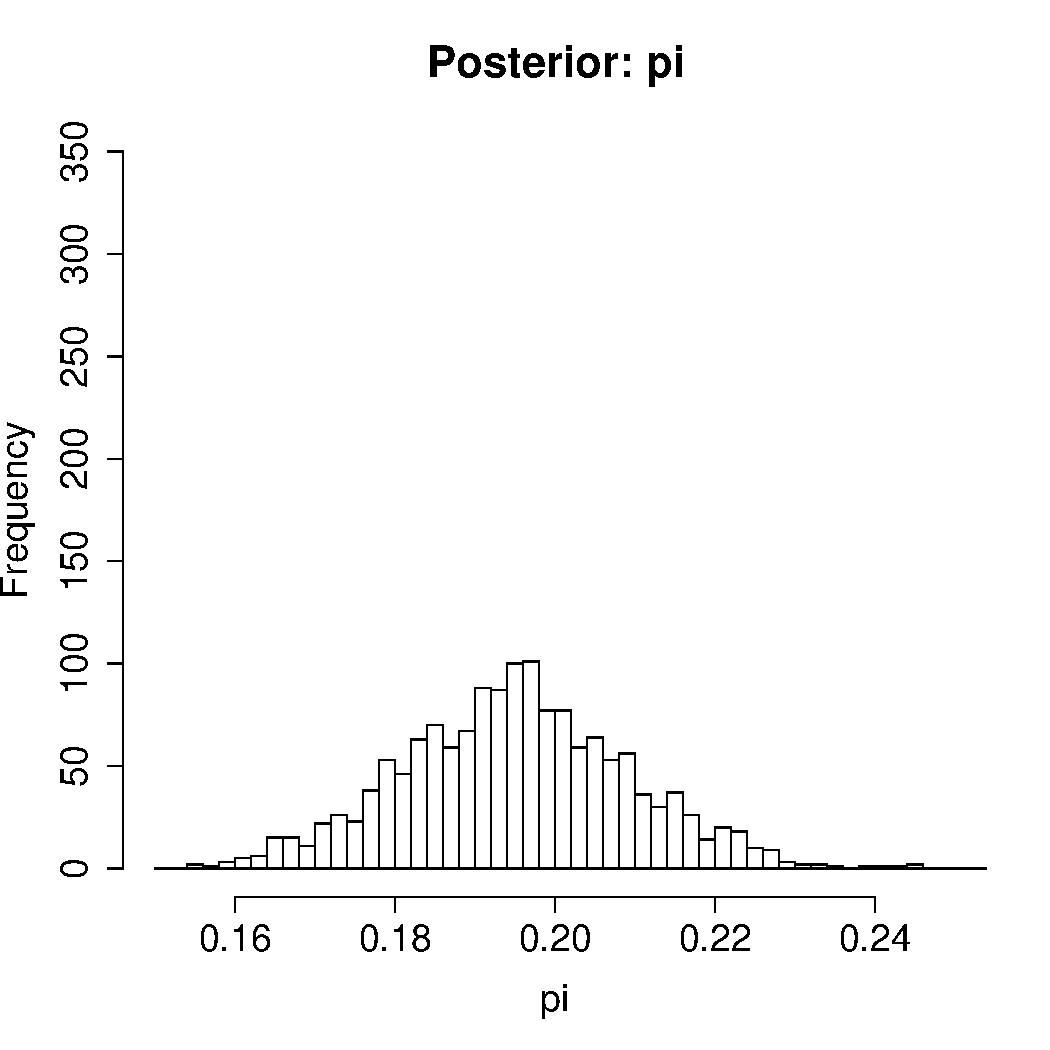
\includegraphics[width=0.40\textwidth]{pdf/binomial-posterior-pi.pdf}%
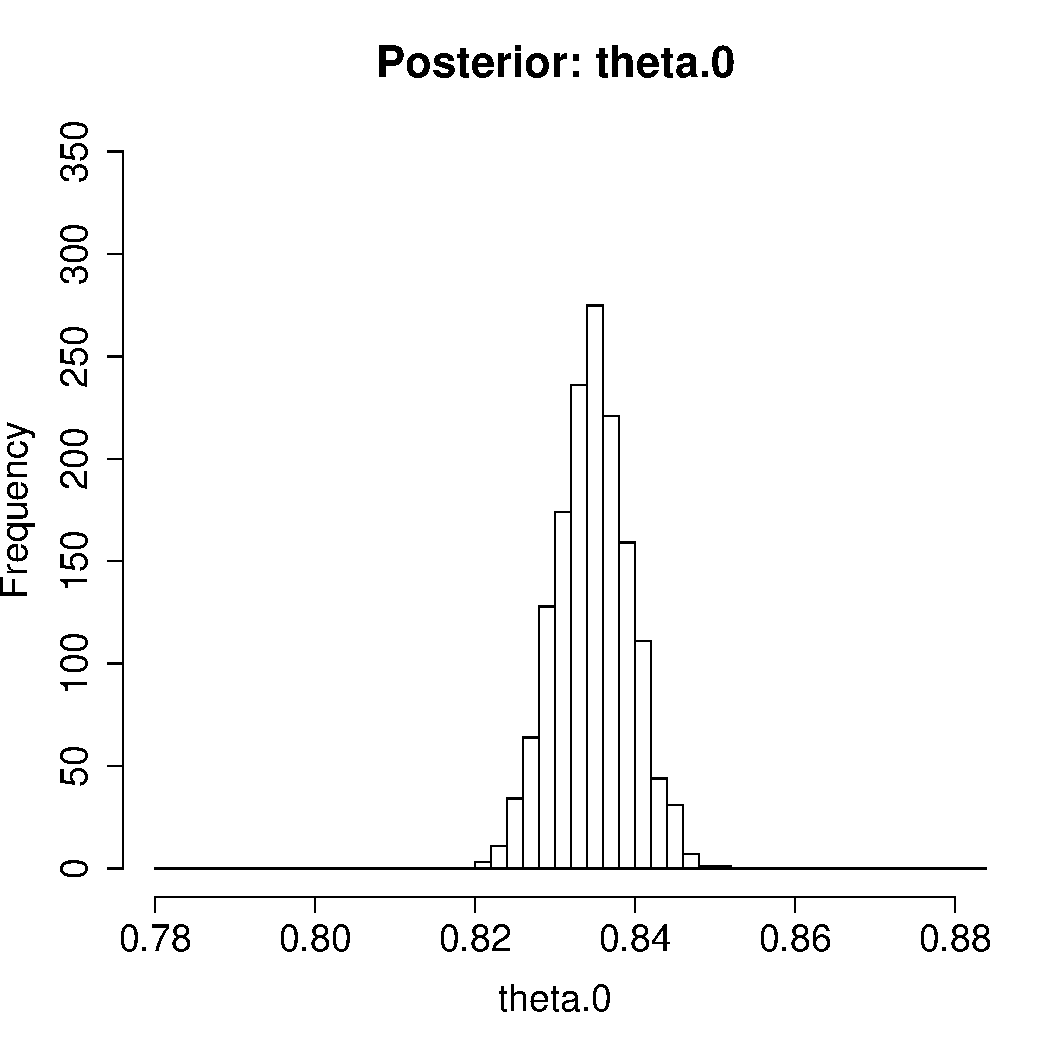
\includegraphics[width=0.40\textwidth]{pdf/binomial-posterior-theta0.pdf}%
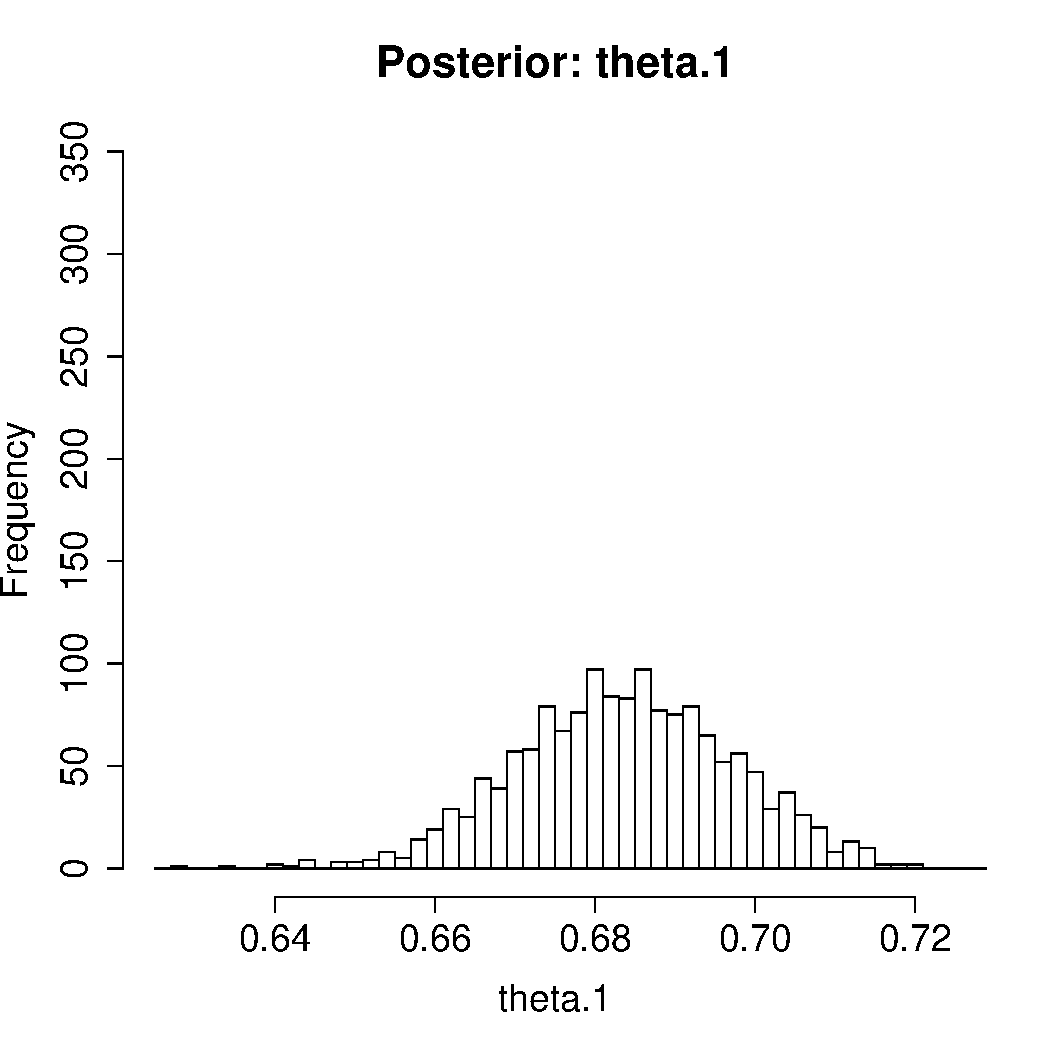
\includegraphics[width=0.40\textwidth]{pdf/binomial-posterior-theta1.pdf}
\end{center}
\begin{center}
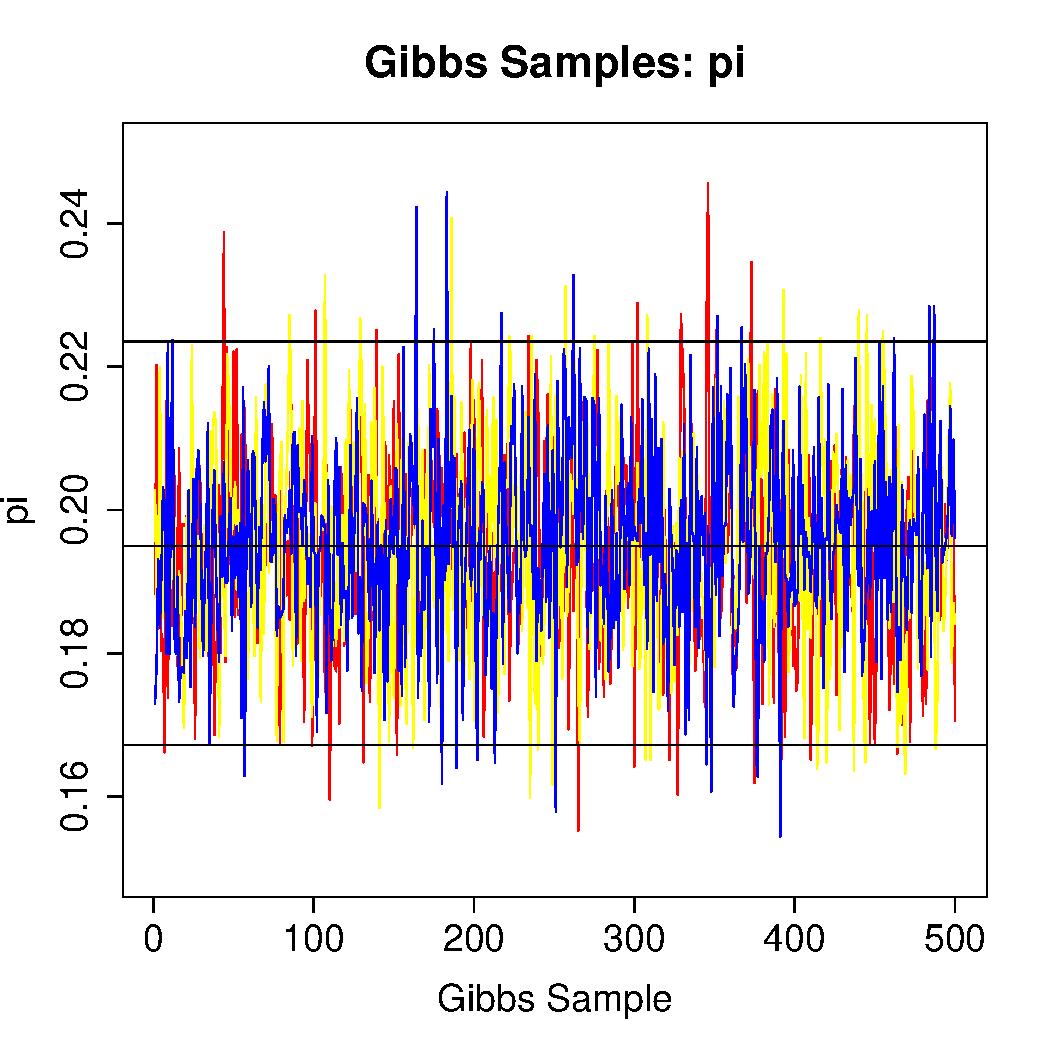
\includegraphics[width=0.4\textwidth]{pdf/binomial-traceplot-pi.pdf}%
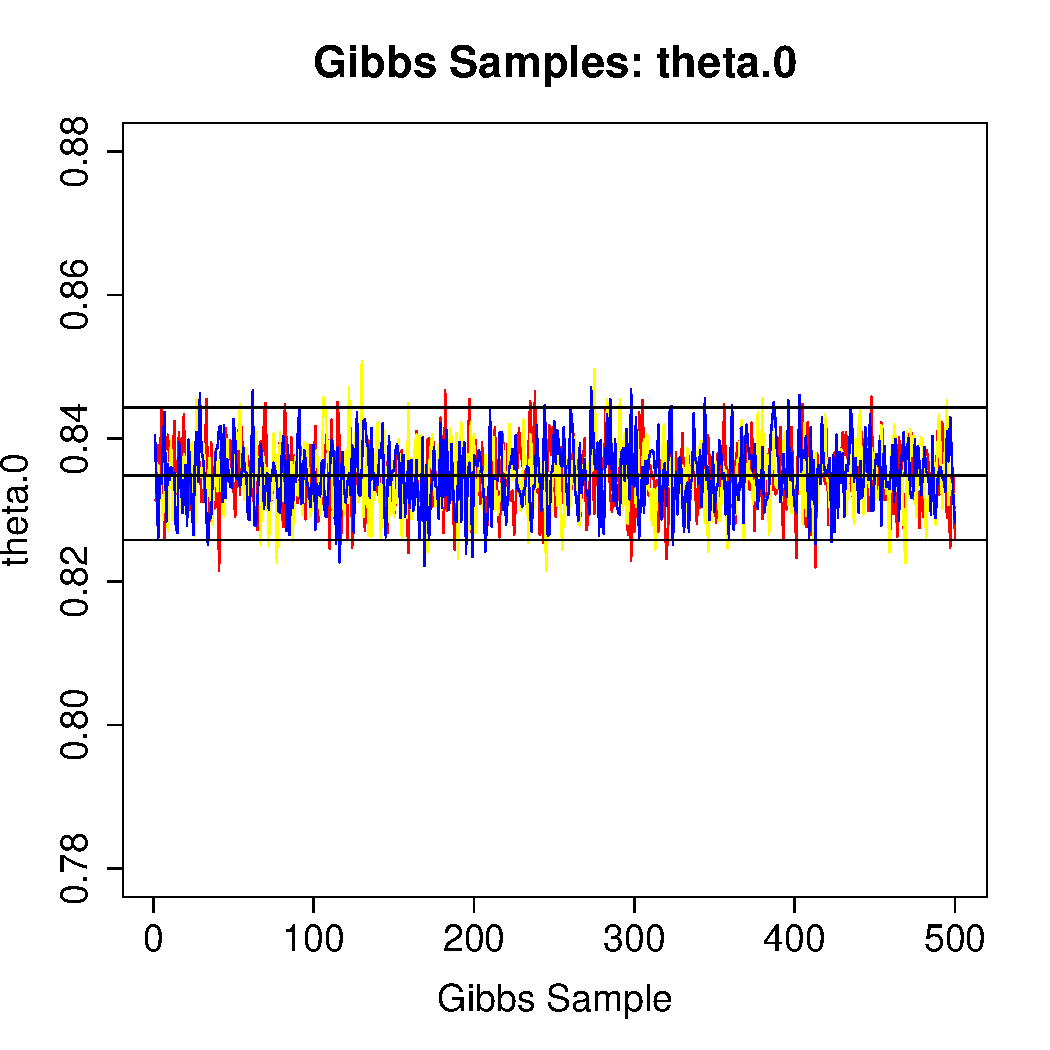
\includegraphics[width=0.4\textwidth]{pdf/binomial-traceplot-theta0.pdf}%
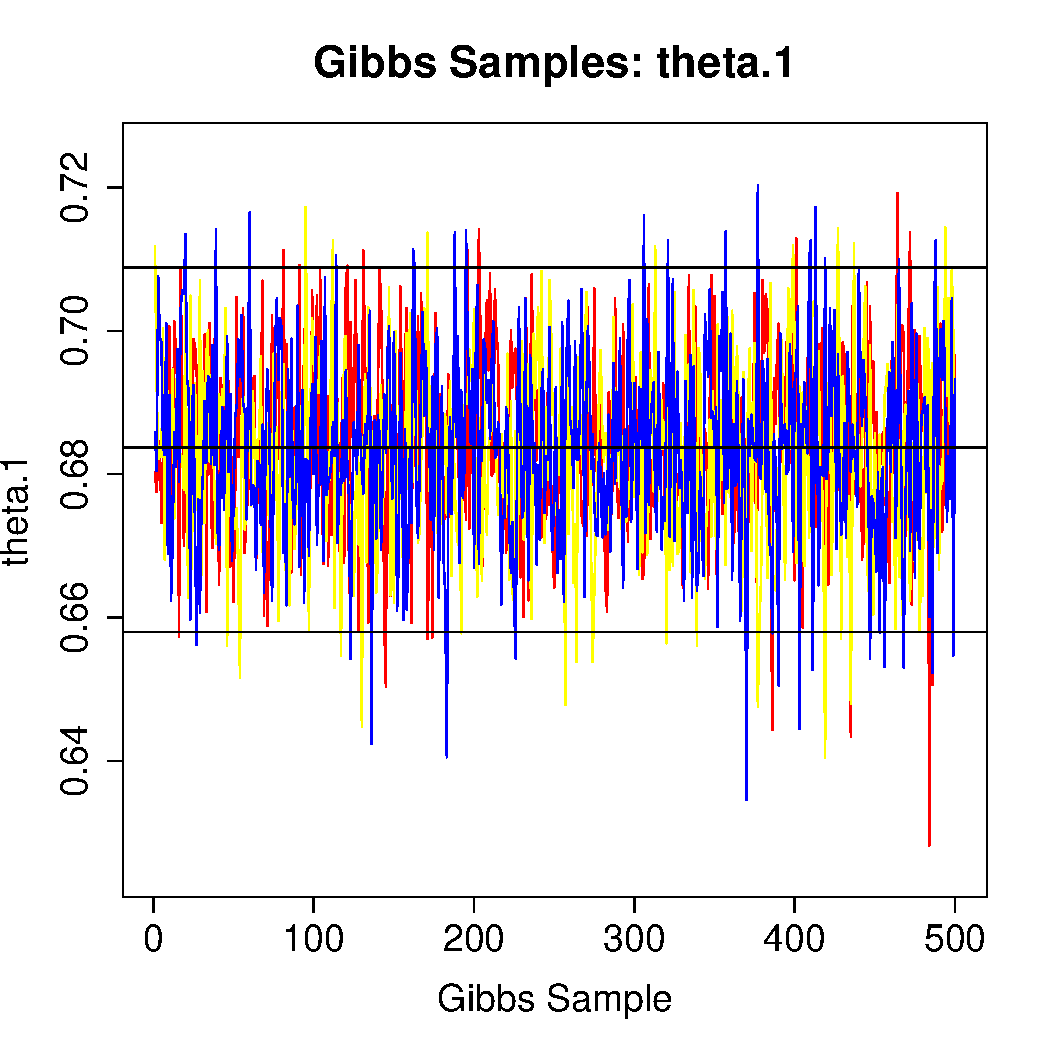
\includegraphics[width=0.4\textwidth]{pdf/binomial-traceplot-theta1.pdf}%
\end{center}
\mycaption{Binomial model: posterior histograms and traceplots.
Simulated model parameters being estimated are
$\pi=0.2$, $\theta_0 = 0.83$ and $\theta_1=0.71$.}%
\label{binomial-posterior.fig}
\end{figure}
%
Histograms of the posterior samples for $\pi$, $\theta_0$ and
$\theta_1$ for the binomial model from Figure~\ref{binomial-model.fig}
are shown in Figure~\ref{binomial-posterior.fig}.  These are all very
tightly centered on the values used for the simulation.  The second
row is a traceplot of the sampled values for the same three parameters
as in the last figure.  These are all of the samples after the 500
sample burn-in period.  Each plot represents three Markov chains,
which can be seen to be mixed very well in that they explore
overlapping parts of the parameter space.

All plots are on the same vertical and horizontal scale, showing
$\theta_0$ to be much more tightly estimated than $\pi$ or $\theta_1$.
There are roughly four times as many data points for $\theta_1$ than
$\theta_0$ with a sampled prevalence $\pi = 0.2$.  The number of data
points used for $\theta_0$ is $0.5 \cdot 0.8 I J = 8000$, for
$\theta_1$ it is $0.5 \cdot 0.2 I J = 2000$ and for $\pi$ it is $I =
1000$ data points.

\begin{figure}
\begin{center}
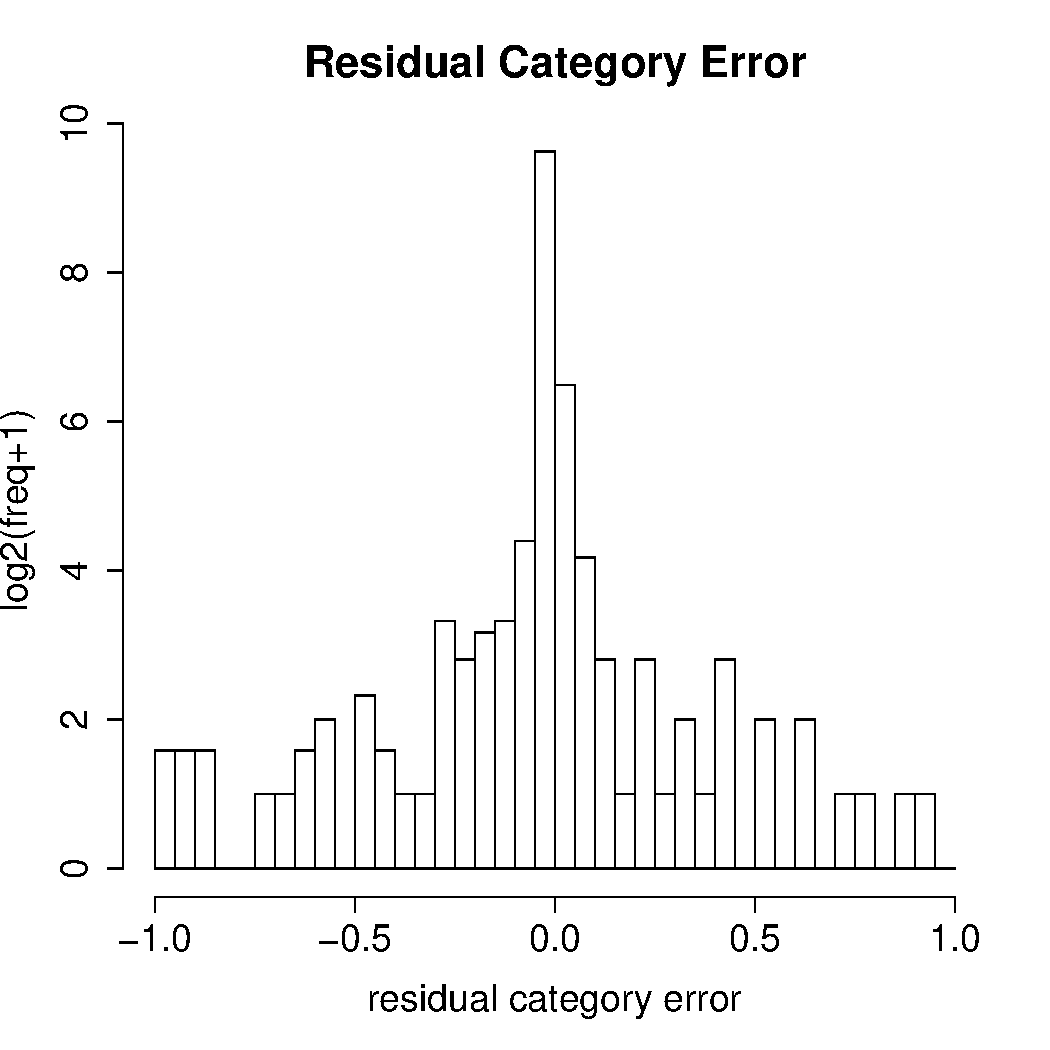
\includegraphics[width=0.4\textwidth]{pdf/binomial-cat-residual.pdf}%
\end{center}
\mycaption{Binomial model: histogram of residual errors in category prediction, which is the
difference between the estimated probability of a category and the true
category, which we know from the simulation.  The plot is on a log (base 2)
scale, with 1 added to counts.}%
\label{binomial-cat-residual.fig}
\end{figure}
%
Figure~\ref{binomial-cat-residual.fig} shows the residual errors made
by the model.  The counts in the histogram are of residual errors,
where the error for item $i$ is defined by
\[
e_i = c_i - P(c_i = 1|x)
\]
or equivalently $c_i = P(c_i = 1|x_i) + e_i$.  The probability
$P(c_i=1|x)$ is estimated using sampled category assignments from the
joint posterior $p(c,\pi,\theta_0,\theta_1|x)$, which effectively
integrates out the parameter estimates for $\pi$, $\theta_0$ and
$\theta_1$.

Of the 1000 examples, 23 of them would be assigned the wrong category
in that the absolute error is greater than 0.5.  There will be fewer
errors with more annotators or with more accurate annotators.

The
expected result of adding more annotators is easily estimated, because
all new annotators have the same ability in the model.


\subsection{Simulated Beta-Binomial by Annotator}


\begin{figure}
\begin{center}
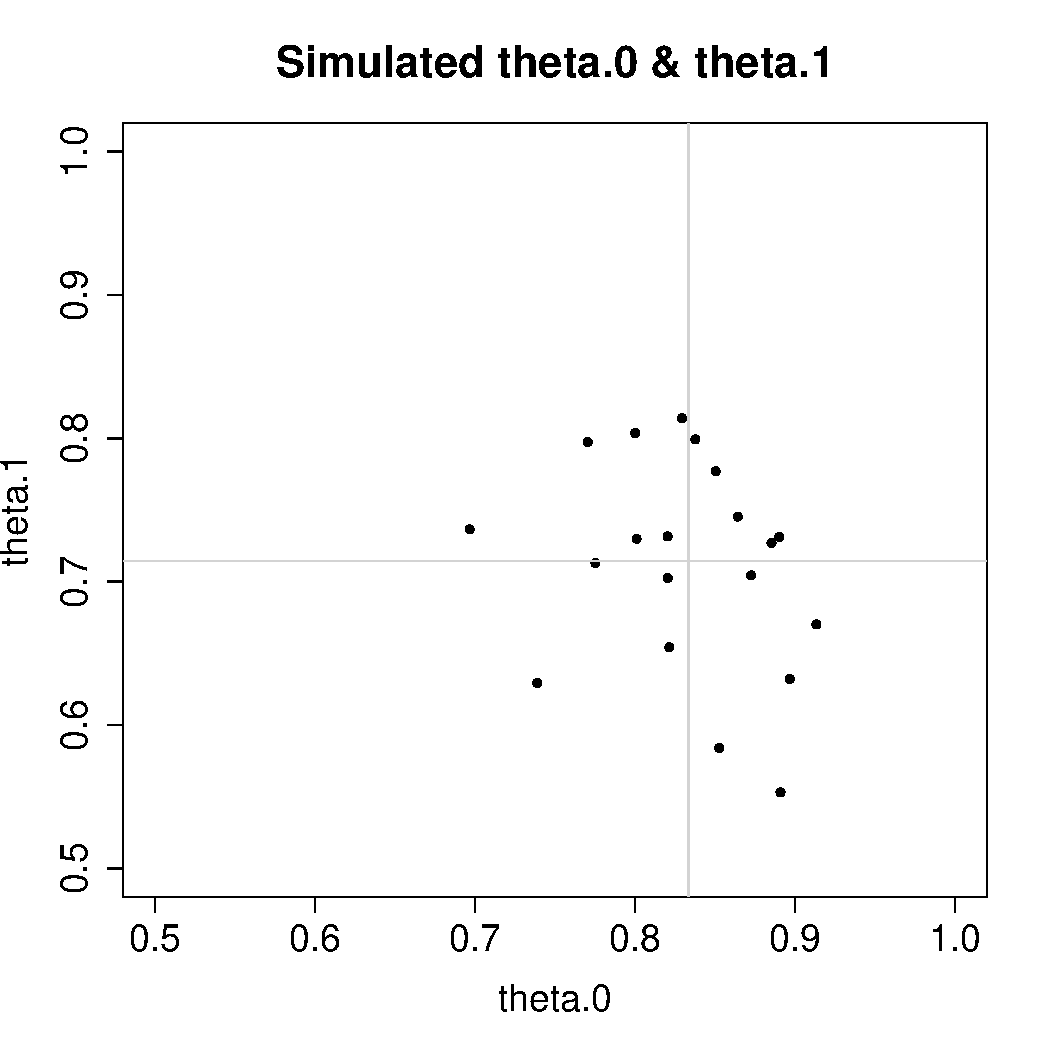
\includegraphics[width=0.4\textwidth]{pdf/beta-binomial-anno-sim-thetas.pdf}%
\end{center}
\mycaption{Beta binomial by annotator model: 20 sampled values of $\theta_0$ and $\theta_1$ for the
beta-binomial by annotator model generated from beta distributions
$\theta_0 \sim \mathsf{Beta}(40,8)$ and $\theta_1 \sim \mathsf{Beta}(20,8)$.
The horizontal and vertical lines are placed at the means of the respective beta distributions.}\label{theta-scatter-by-anno.fig}.
\end{figure}
%
The beta-binomial by annotator model outlined in
Figure~\ref{beta-binomial-anno-model.fig} also fits very well with large
amounts of simulated data.  As with the previous model, we simulated
20 annotators over 1000 items with a 50\% missingness at random rate.
The prevalence was simulated at $\pi = 0.20$, and the multilevel
parameters at $(\alpha_0,\beta_0) = (40,8)$ and $(\alpha_1,\beta_1) =
(20,8)$.  The specificity and sensitivity parameters were then drawn
from a beta distribution, resulting in the set of values shown
in Figure~\ref{theta-scatter-by-anno.fig}.

\begin{figure}
\begin{center}
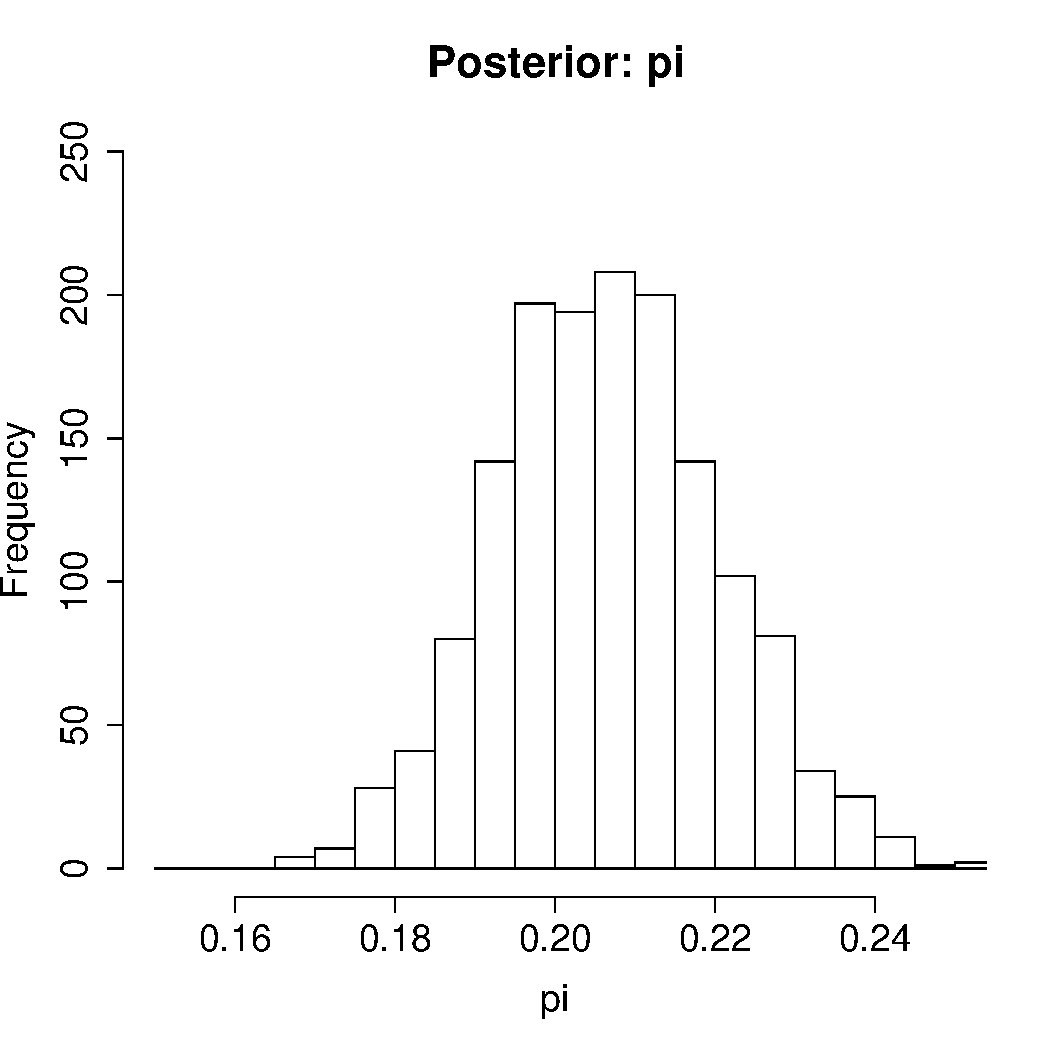
\includegraphics[width=0.4\textwidth]{pdf/beta-binomial-anno-posterior-pi.pdf}%
\end{center}
\mycaption{Beta binomial by annotator model: histogram of the posterior distribution of prevalence
parameter $\pi$.   The simulated value was $\pi=0.2$ and the sample
prevalence was 0.206.}%
\label{beta-binomial-anno-posterior-pi.fig}
\end{figure}
%
In Figure~\ref{beta-binomial-anno-posterior-pi.fig}, we show the
posterior distribution for the prevalence parameter $\pi$.  It is very
similar to the posterior distribution for the binomial model shown in
Figure~\ref{binomial-posterior.fig}.

\begin{figure}
\begin{center}
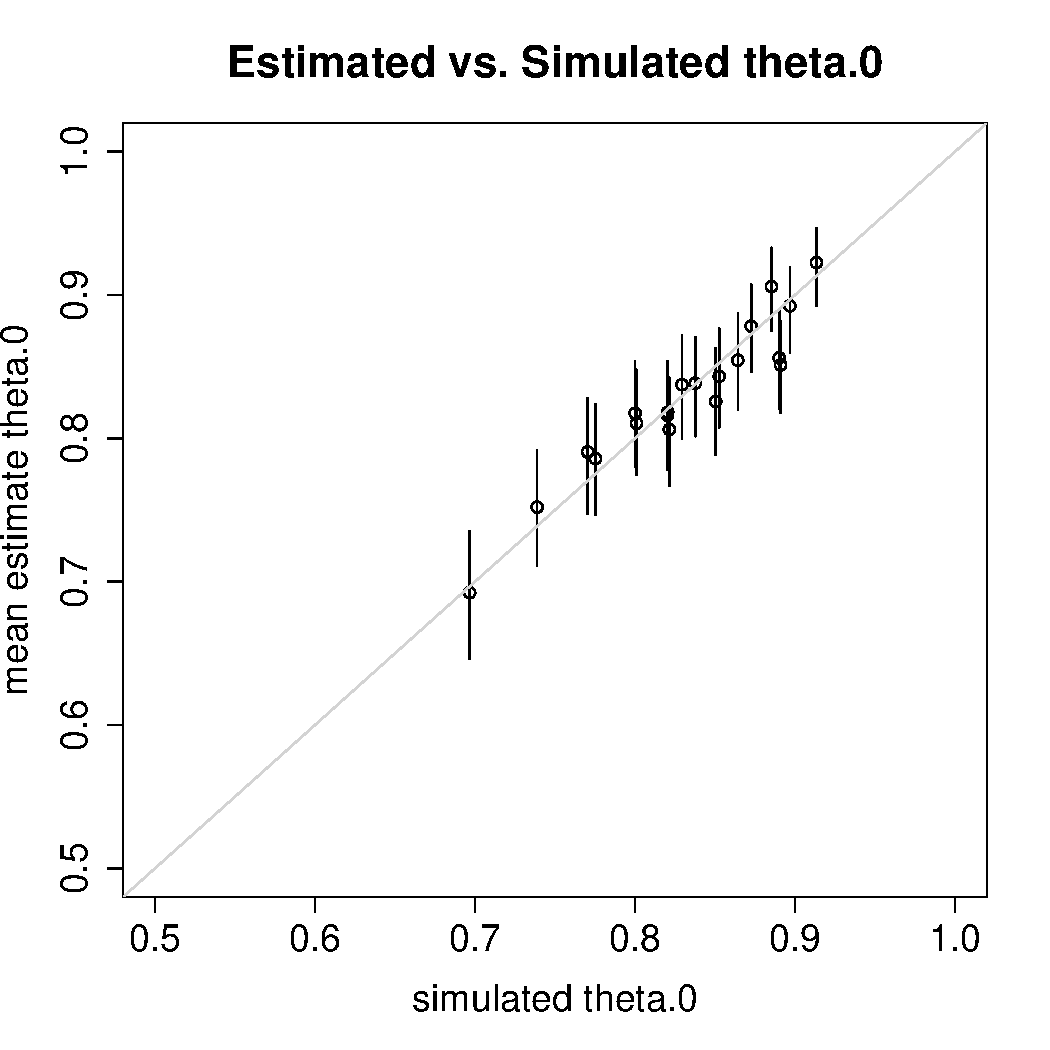
\includegraphics[width=0.4\textwidth]{pdf/beta-binomial-anno-theta0-fit.pdf}%
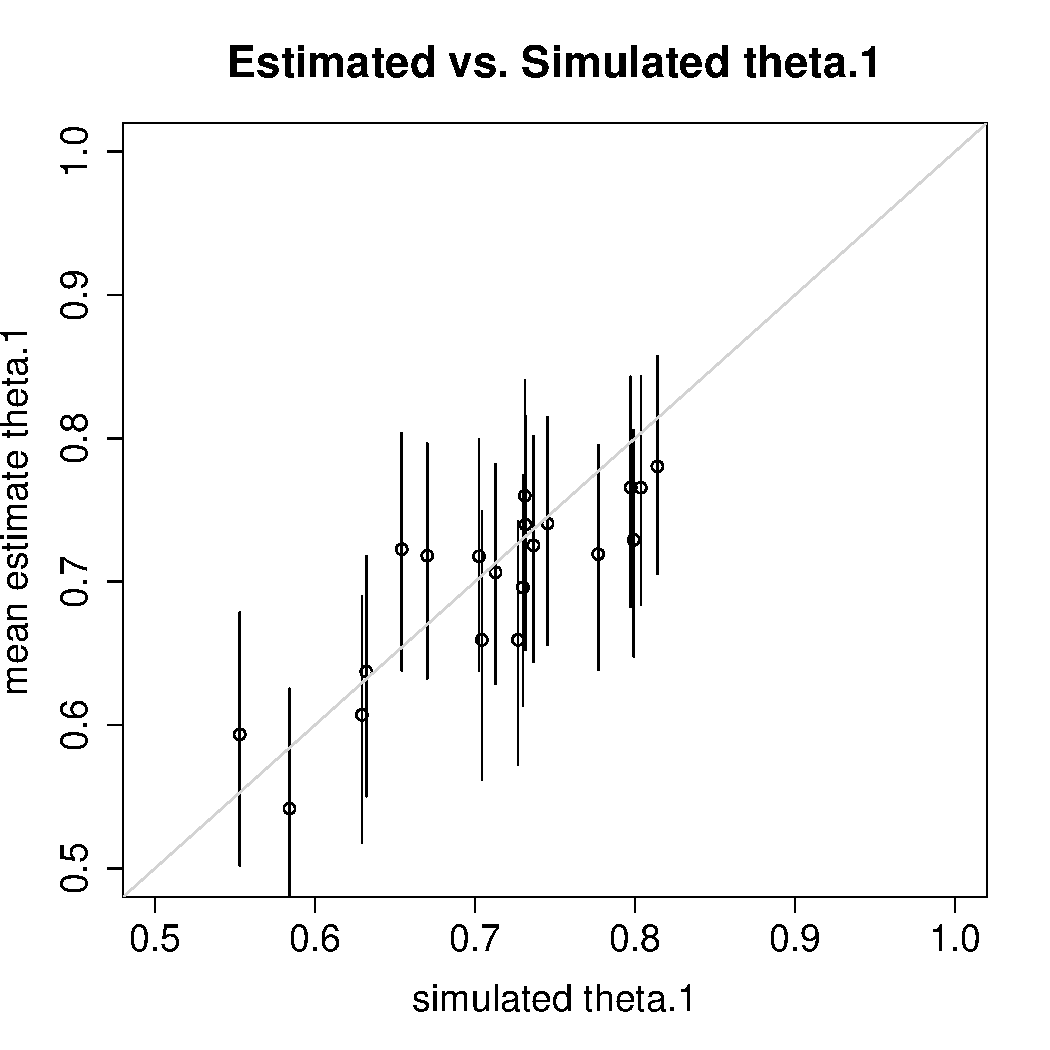
\includegraphics[width=0.4\textwidth]{pdf/beta-binomial-anno-theta1-fit.pdf}%
\end{center}
\mycaption{Beta binomial by annotator model: posterior mean and 95\% intervals for
$\theta_0$ and $\theta_1$.  Points are arranged on the horizontal axis
according to their simulated values, with the vertical representing the
estimates.  The circles are mean estimates and the bars are 95\% posterior
intervals.  The 45 degree line represents perfect estimation. }%
\label{beta-binomial-anno-thetas-fit.fig}
\end{figure}
%
Figure~\ref{beta-binomial-anno-thetas-fit.fig} shows how well the
posterior estimates match the simulated true values.  With 20
annotators, we would expect one true value to not lie within the
estimated 95\% interval per graph.  As expected, the posterior
intervals for the sensitivity estimates are wider than for specificity.

\begin{figure}
\begin{center}
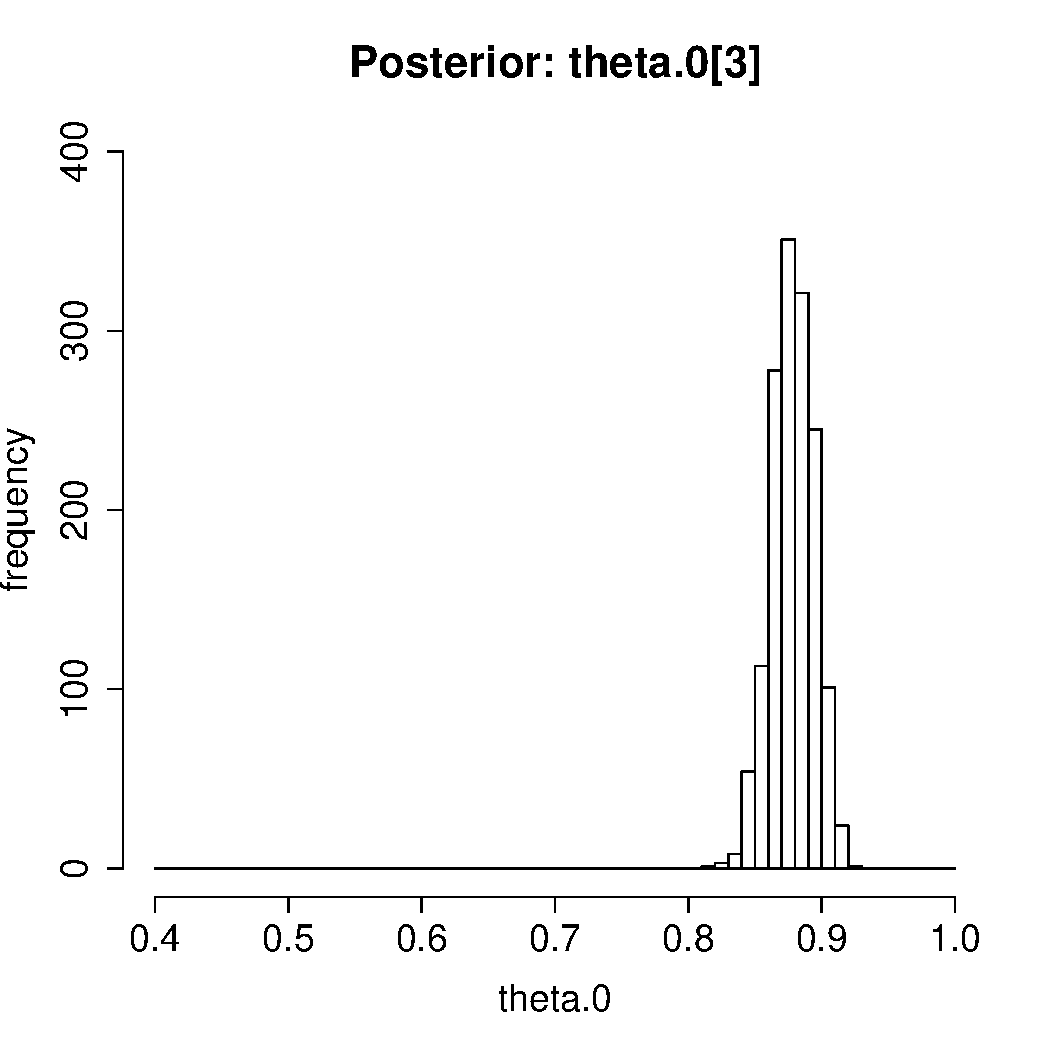
\includegraphics[width=0.4\textwidth]{pdf/beta-binomial-anno-post-theta0.pdf}%
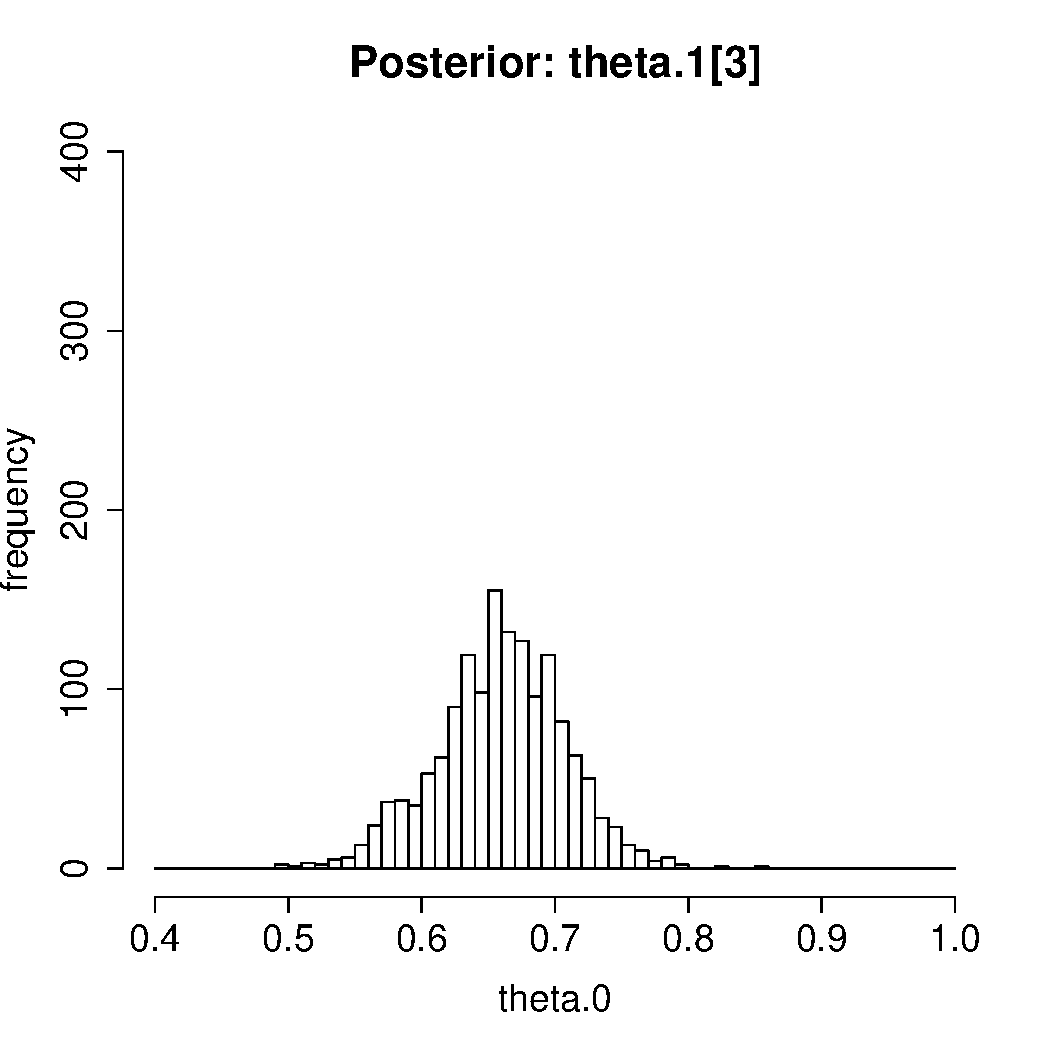
\includegraphics[width=0.4\textwidth]{pdf/beta-binomial-anno-post-theta1.pdf}
\end{center}
\mycaption{Beta-binomial by annotator model: posterior fits of a sample annotator's sensitivity and
specificity parameters in the beta-binomial by annotator model.
The simulated values were $\theta_{0,3}=0.87$ and $\theta_{1,3}=0.70$.}\label{beta-binomial-anno-post-thetas.fig}
\end{figure}
%
A 95\% posterior interval only summarizes the posterior distribution.
In Figure~\ref{beta-binomial-anno-post-thetas.fig}, we show the
estimates of specificity and sensitivity for annotator two, namely
$\theta_{0,3}$ and $\theta_{1,3}$.  As can be seen from the similarly
scaled histograms, the estimate of the sensitivity parameter
$\theta_{1,3}$ is much more uncertain than that of the specificity
parameter, with a posterior 95\% interval for $\theta_{0,3}$ of
$(0.84,0.91)$ and for $\theta_{1,3}$ of $(0.56,0.76)$.  This is
expected because $\theta_0$ has roughly four times as much data on
which to base an estimate than $\theta_1$, so should have about half
as much posterior deviation all else being equal.  Further note that
these intervals are wider than they would be for simple binomial
estimates given known data.  As annotators accrue more annotations
overall, the posterior interval for accuracy becomes tighter.

\begin{figure}
\begin{center}
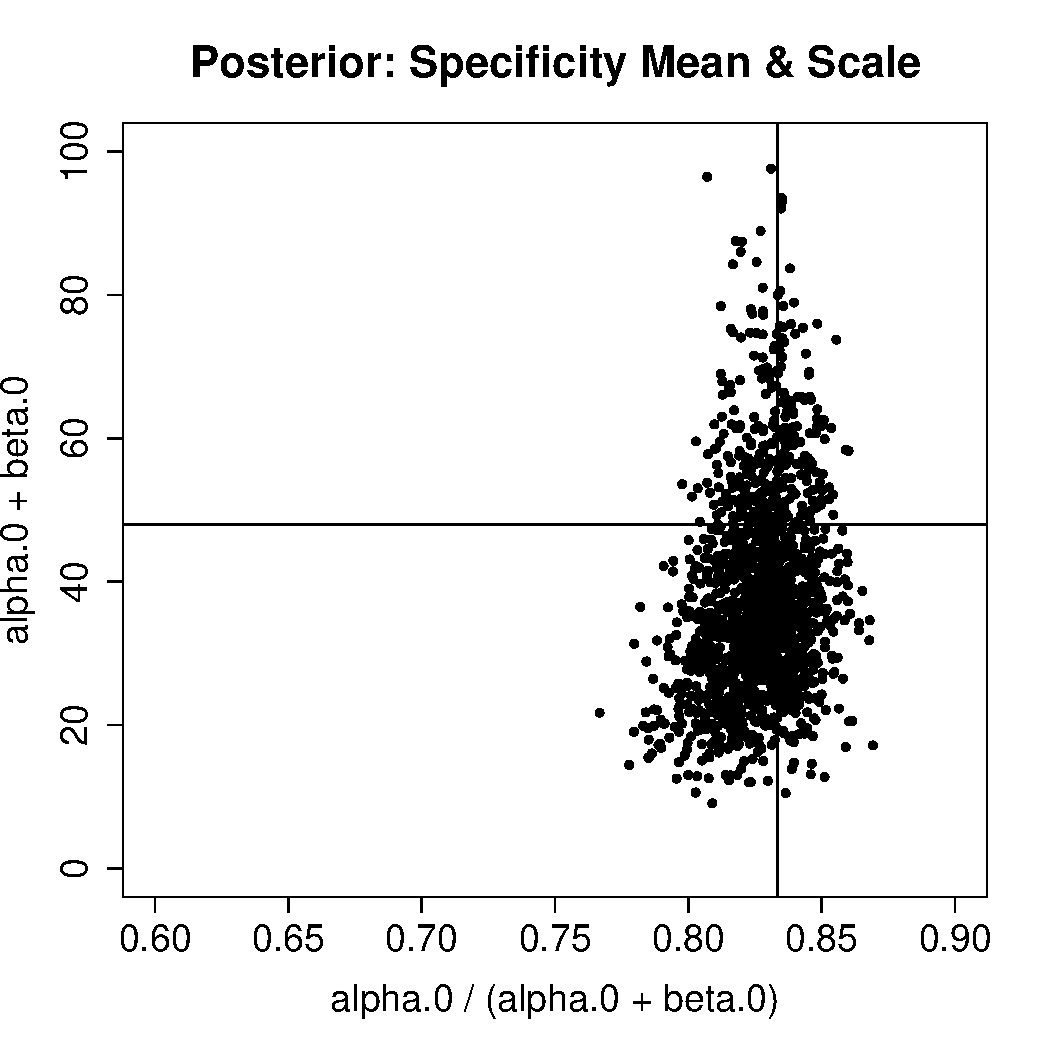
\includegraphics[width=0.4\textwidth]{pdf/beta-binomial-anno-scatter-spec.pdf}%
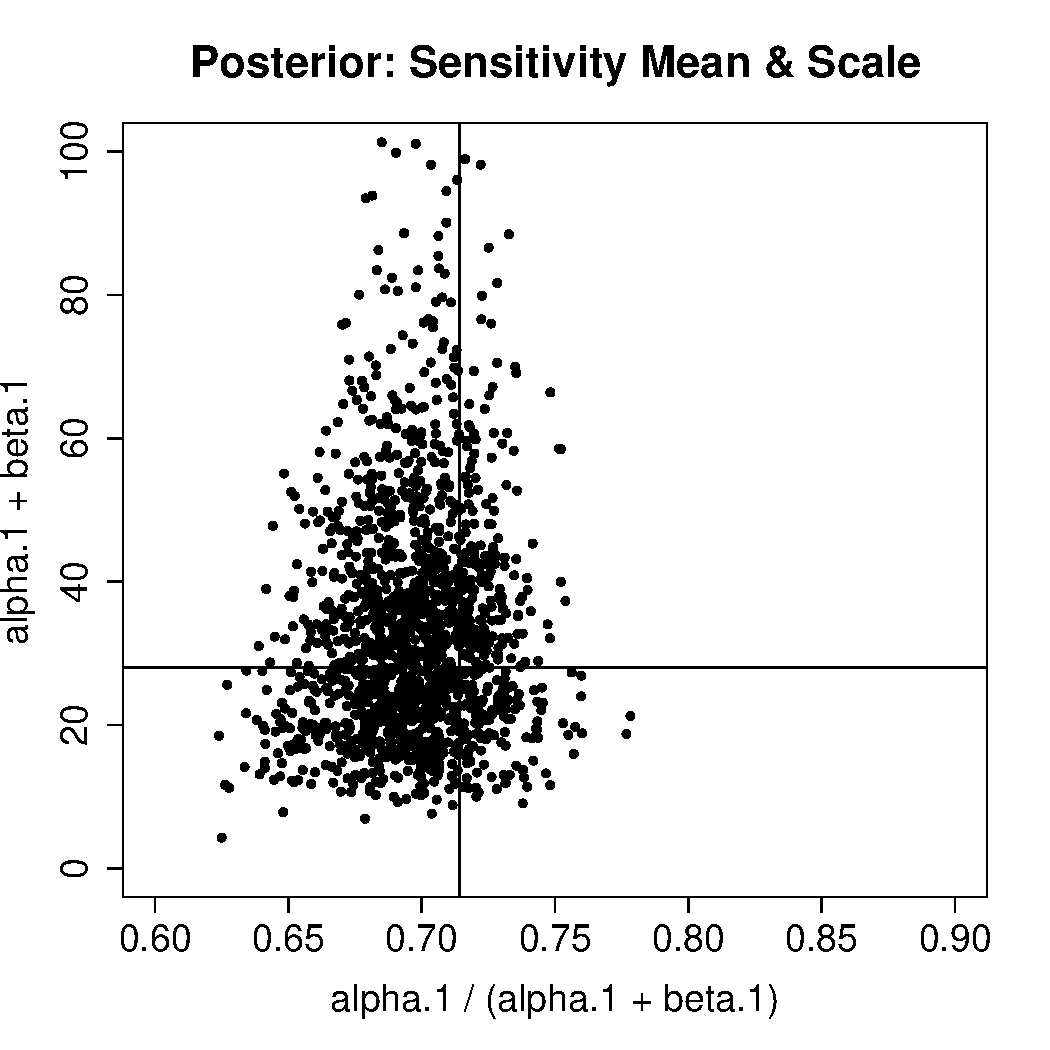
\includegraphics[width=0.4\textwidth]{pdf/beta-binomial-anno-scatter-sens.pdf}
\end{center}
\mycaption{Beta-binomial by annotator model: posterior distribution for the specificity and sensitivity beta priors in
the beta-binomial by annotator model.  The values are parameterized in
terms of scale $alpha + \beta$ and mean $\alpha/(\alpha+\beta)$.    The
lines are drawn at the simulated values of the parameters.}\label{beta-binomial-anno-beta-fits.pdf}
\end{figure}
%
To see how well the model is able to recover the beta parameters used
to generate the data, Figure~\ref{beta-binomial-anno-beta-fits.pdf}
shows a scatterplot of posterior samples for the beta parameters
reparameterized as scales and means.  As can be seen from the figure,
the specificity (category 0) estimates are tighter than the
sensitivity (category 1) estimates, because there is four times as
much category 0 data with a prevalence of $\pi=0.2$.

In all of these models, it is important to realize that the lack of
centering on the simulated value is not evidence of bias.  Rather, it
reflects the variance of the underlying sampling.  For instance, the
sample count of category 1 items will be distributed as a binomial
with parameter $\pi$, which has a deviation of $\sqrt{I \pi (1 -
\pi)}$, or about 17 when $I=2000$ and $\pi=0.2$ as in this example.
17 cases going one way or the other make a difference of 1\% in
prevalence.  In the simulation for this section, the number of 1
categories was 414/2000, or 20.7\%.  The mean value of posterior
samples for $\pi$ was 0.207, which indicates that the model's fitting
the empirical distribution very closely.  The histogram of posterior
$\pi$ simulations looks almost identical to the one in the previous
section.  The only way to tighten these estimates is with more
items being classified.

\begin{figure}
\begin{center}
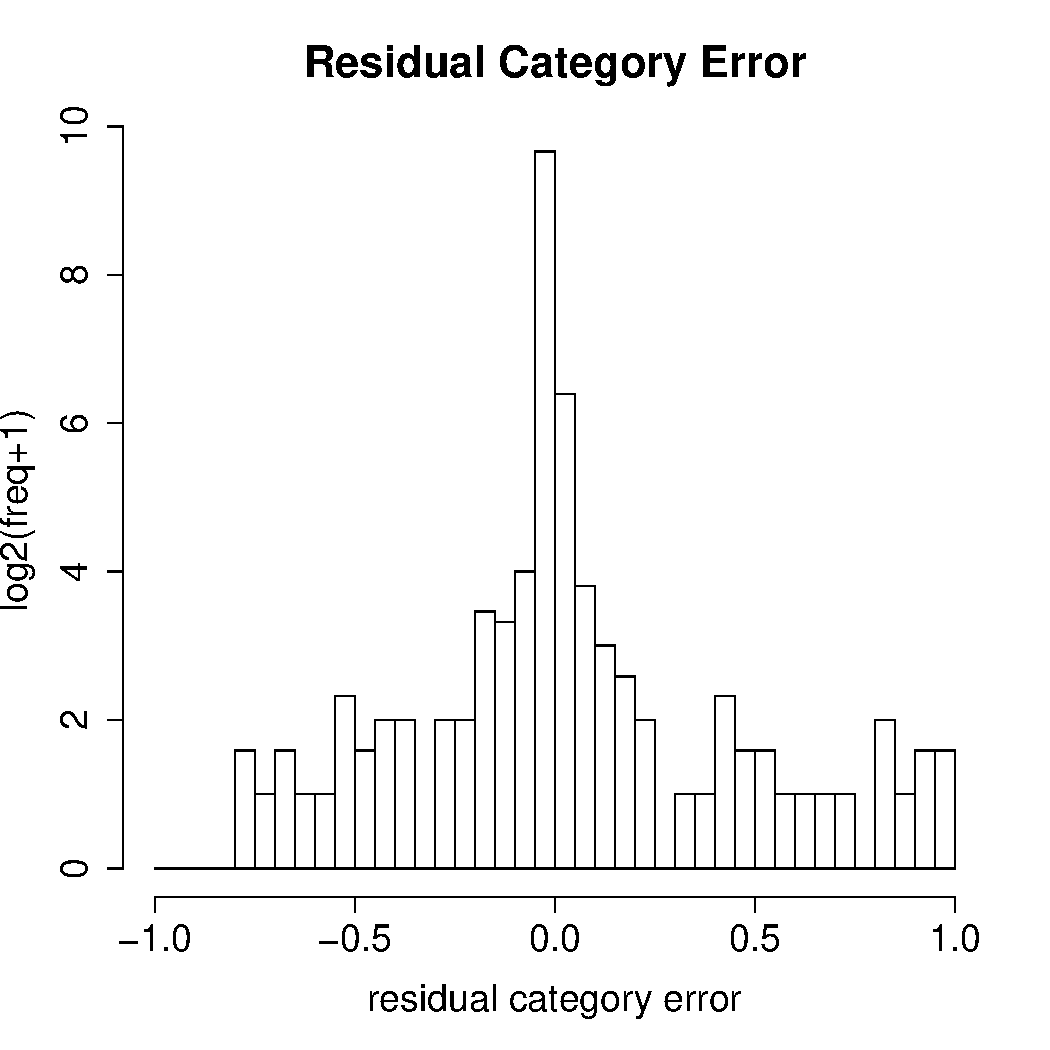
\includegraphics[width=0.4\textwidth]{pdf/beta-binomial-anno-cat-residual.pdf}%
\end{center}
\mycaption{Beta-binomial by annotator model: histogram of residual errors in category
prediction, which is the difference between the estimated probability
of a category and the true category, which we know from the
simulation.  The plot is on a log (base 2) scale, with 1 added to
counts.}%
\label{beta-binomial-anno-cat-residual.fig}
\end{figure}
%
Figure~\ref{beta-binomial-anno-cat-residual.fig} shows the residual
errors made by the model.  This model made 25 errors, which is in the
indistinguishable from the pure binomial model, given that
categorization amounts to a binomial with 1000 trials.  In the limit
as the scale of the beta parameters grows, the beta-binomial models
approach the simple binomial model.




\subsection{Simulated Beta-Binomial by Item}

We simulated the beta-binomial by item model in the same way as the
first two models.  The results we report are very similar to the by
annotator model.  The main difference is that the $\alpha$ and $\beta$
priors have many more instances with which to be estimated (an
expected 800 category 1 and 200 category 0 instances respectively),
but the instances are themselves much more uncertain because they are
being estimated using only the annotators that annotated an item
(an expected 10 per item).


\begin{figure}
\begin{center}
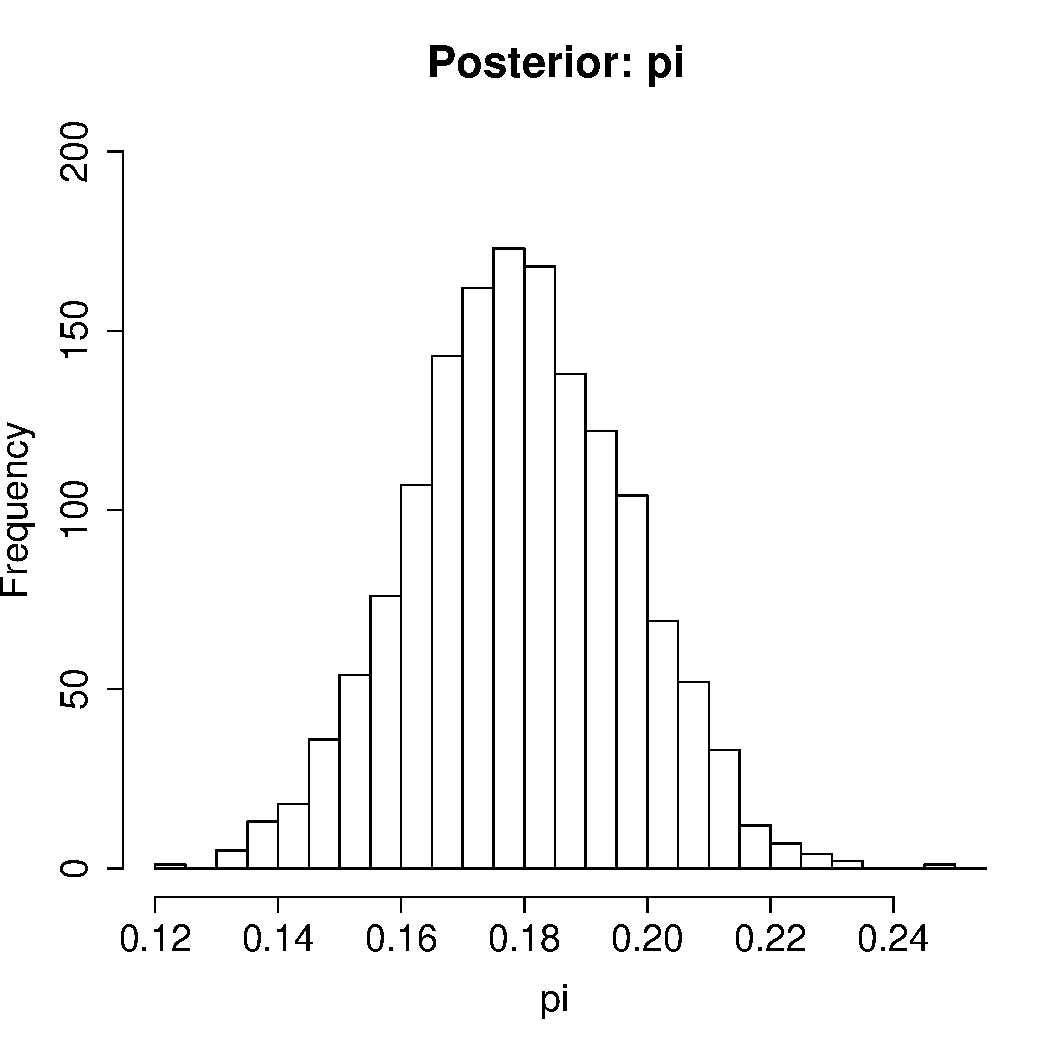
\includegraphics[width=0.4\textwidth]{pdf/beta-binomial-item-posterior-pi.pdf}%
\end{center}
\mycaption{Beta-binomial by item model: Histogram of the posterior prevalence distribution.
The simulated prevalence was $\pi=0.2$ and the empirical prevalence in the
sample was 0.188.}
\label{beta-binomial-item-pi.fig}
\end{figure}
%
The simulated prevalence parameter was $\pi = 0.2$, but only 18.8\% of
the items were category 1 in the sample we drew.  The posterior
calculated by simulation is shown in
Figure~\ref{beta-binomial-item-pi.fig}.

\begin{figure}
\begin{center}
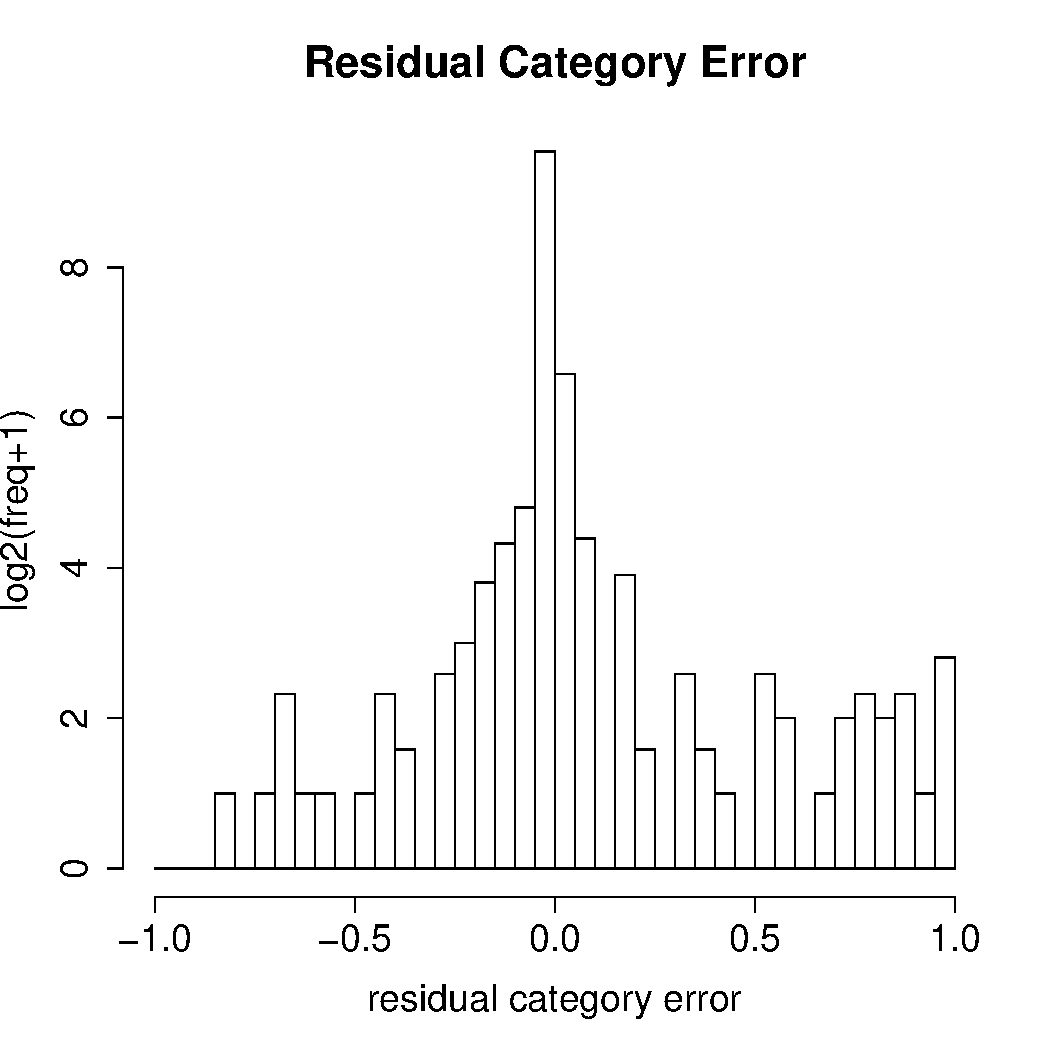
\includegraphics[width=0.4\textwidth]{pdf/beta-binomial-item-cat-residual.pdf}%
\end{center}
\mycaption{Beta-binomial by item: Histogram of reisidual caegory errors.}%
\label{beta-binomial-item-cat-residual.fig}
\end{figure}
%
The category residuals are more uncertain under this model than the
other models, as seen in
Figure~\ref{beta-binomial-item-cat-residual.fig}.  There are now a
total of 38 items which would be misassigned under their most
likely categories.

\begin{figure}
\begin{center}
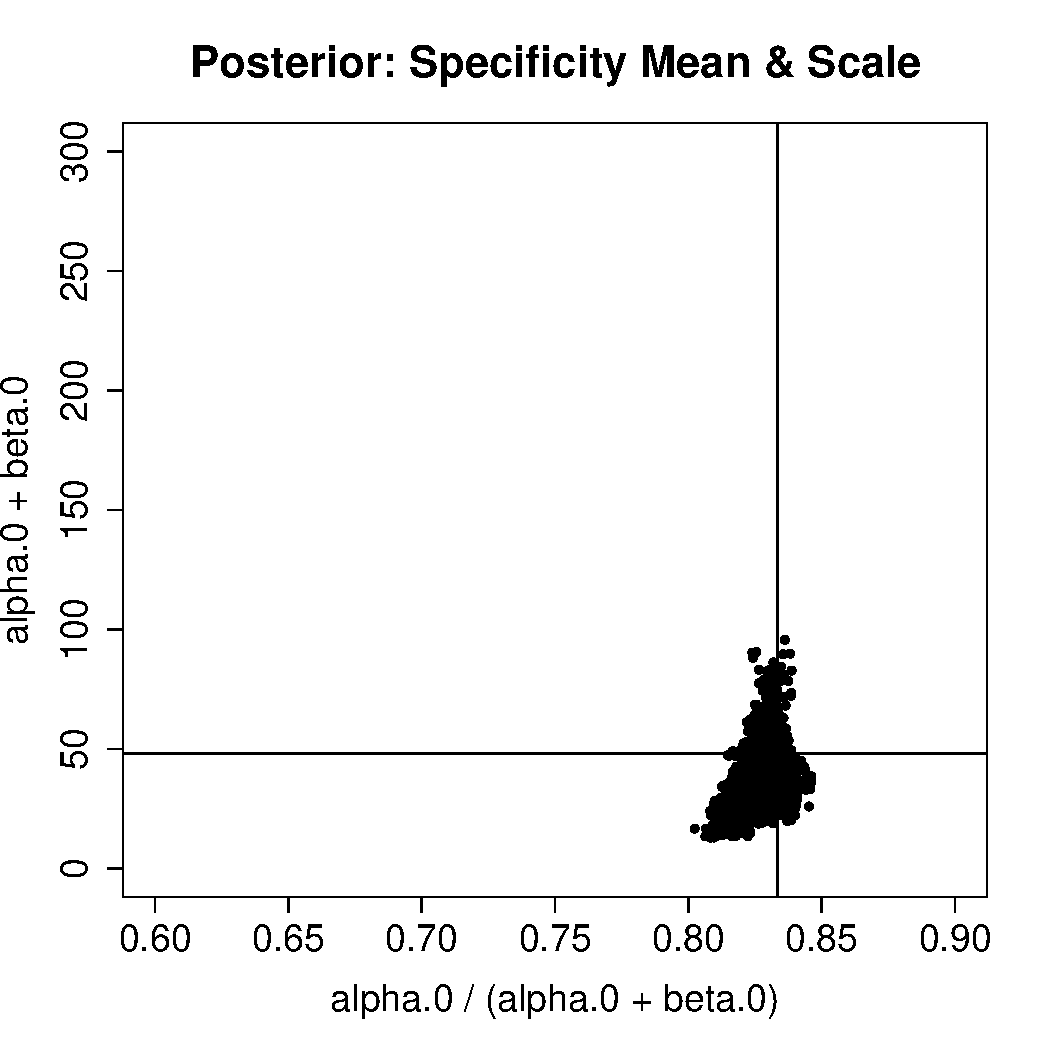
\includegraphics[width=0.4\textwidth]{pdf/beta-binomial-item-scatter-spec.pdf}%
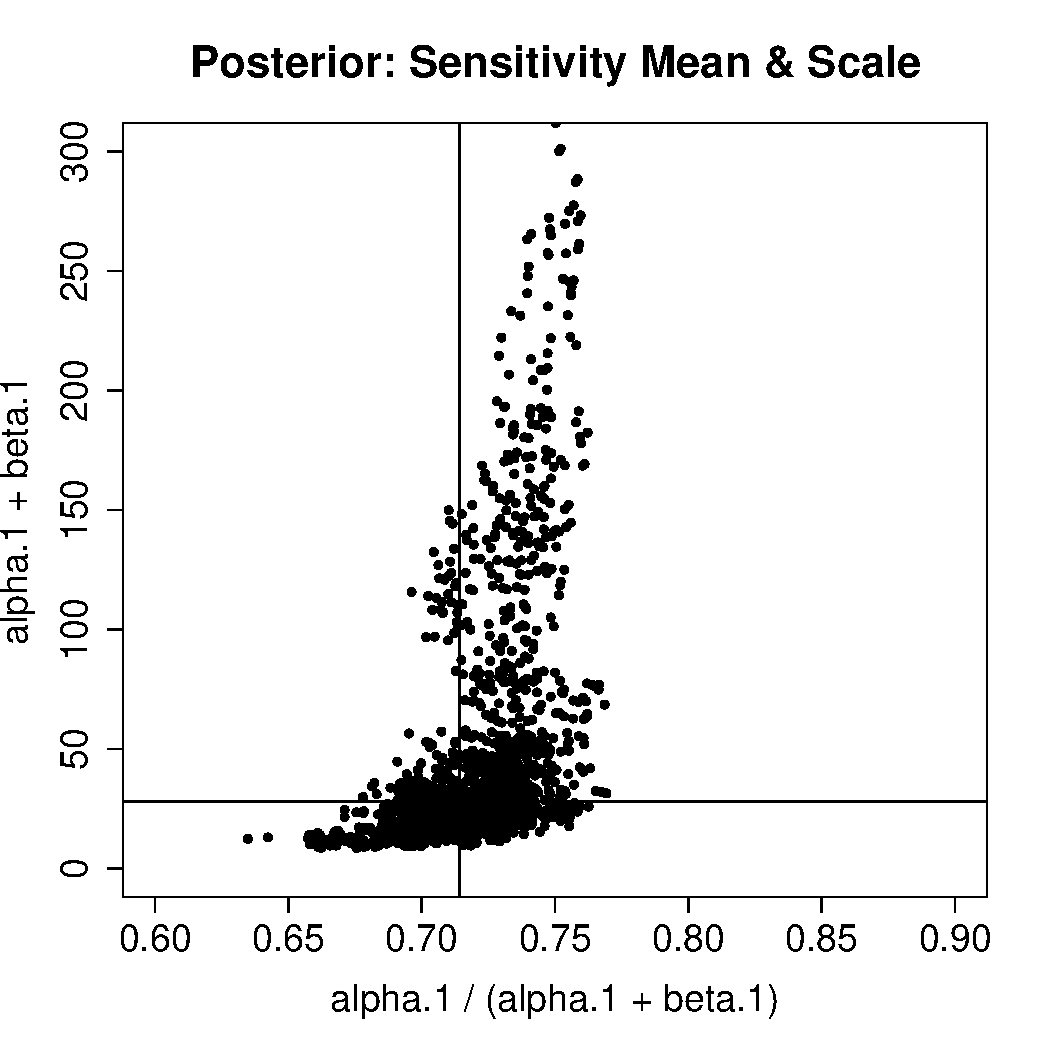
\includegraphics[width=0.4\textwidth]{pdf/beta-binomial-item-scatter-sens.pdf}
\end{center}
\mycaption{Beta-binomial by item model: posterior distribution for the specificity and sensitivity beta priors in
the beta-binomial by item model.  The values are parameterized in
terms of scale $\alpha + \beta$ and mean $\alpha/(\alpha+\beta)$.  The
lines are drawn at the simulated values of the
parameters.}\label{beta-binomial-item-beta-fits.pdf}
\end{figure}
%
The hierarchical aspect of this model, represented as the beta priors
over the item sensitivity or specificity values is not well estimated
with our sample size.  Note how wide the sampled values are for the
scales $\alpha_0+\beta_0$ and $\alpha_1+\beta_1$.  Larger values of
scale parameters reflect variance close to zero.

\begin{figure}
\begin{center}
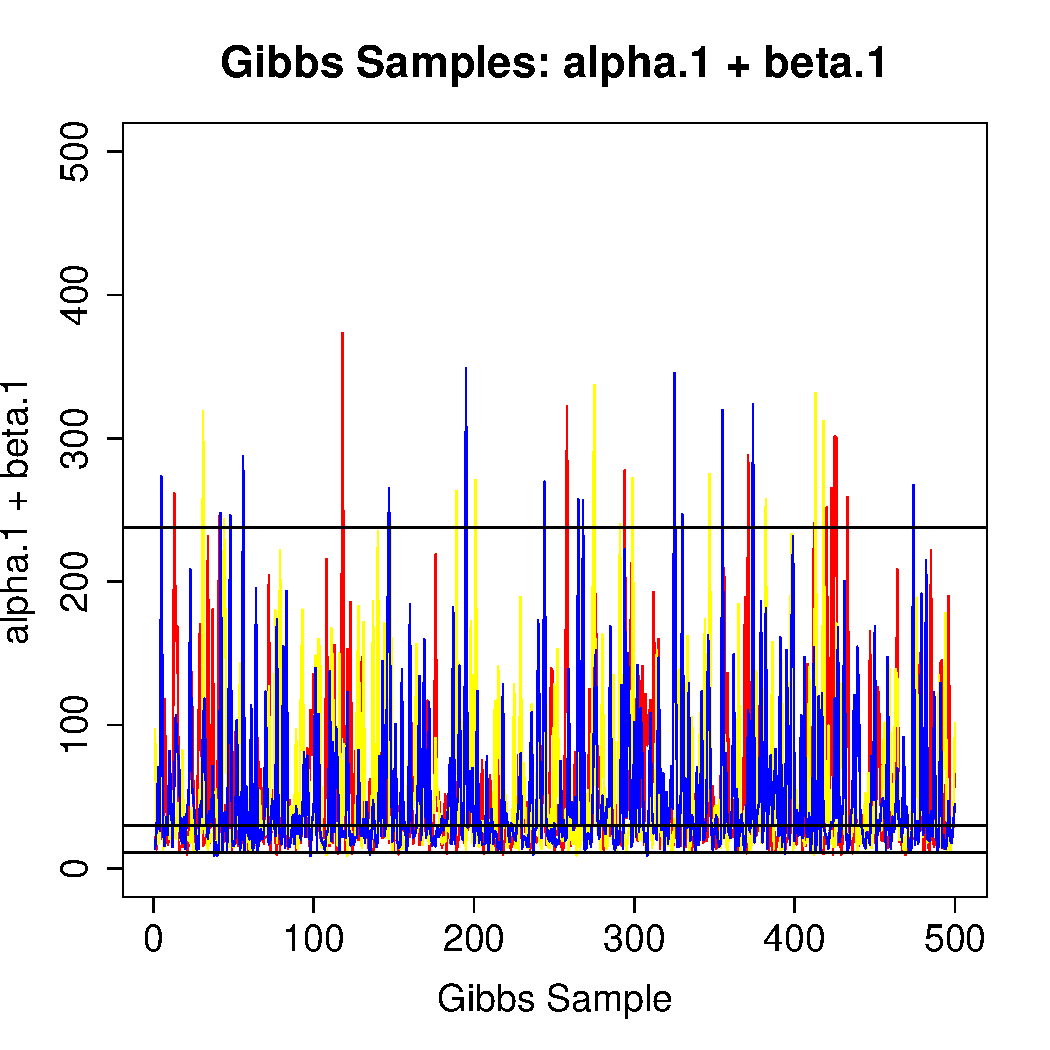
\includegraphics[width=0.4\textwidth]{pdf/beta-binomial-item-traceplot-scale1.pdf}%
\end{center}
\mycaption{Beta-binomial by item: traceplot of $\alpha_1 + \beta_1$ samples from three
independent Markov chains, with horizontal lines around the 95\% intervals and at the
sample median.}%
\label{beta-binomial-item-traceplot-scale1.fig}
\end{figure}
%
The difficulty in fitting the hierarchical parameters is reflected in
the traceplot of samples for $\alpha_1 + \beta_1$, which we show in
Figure~\ref{beta-binomial-item-traceplot-scale1.fig}.  Note how the
median is quite low, but the number of large sampled values is also
high.  With such skewed distributions, median estimates can be much
lower than means.

\begin{figure}
\begin{center}
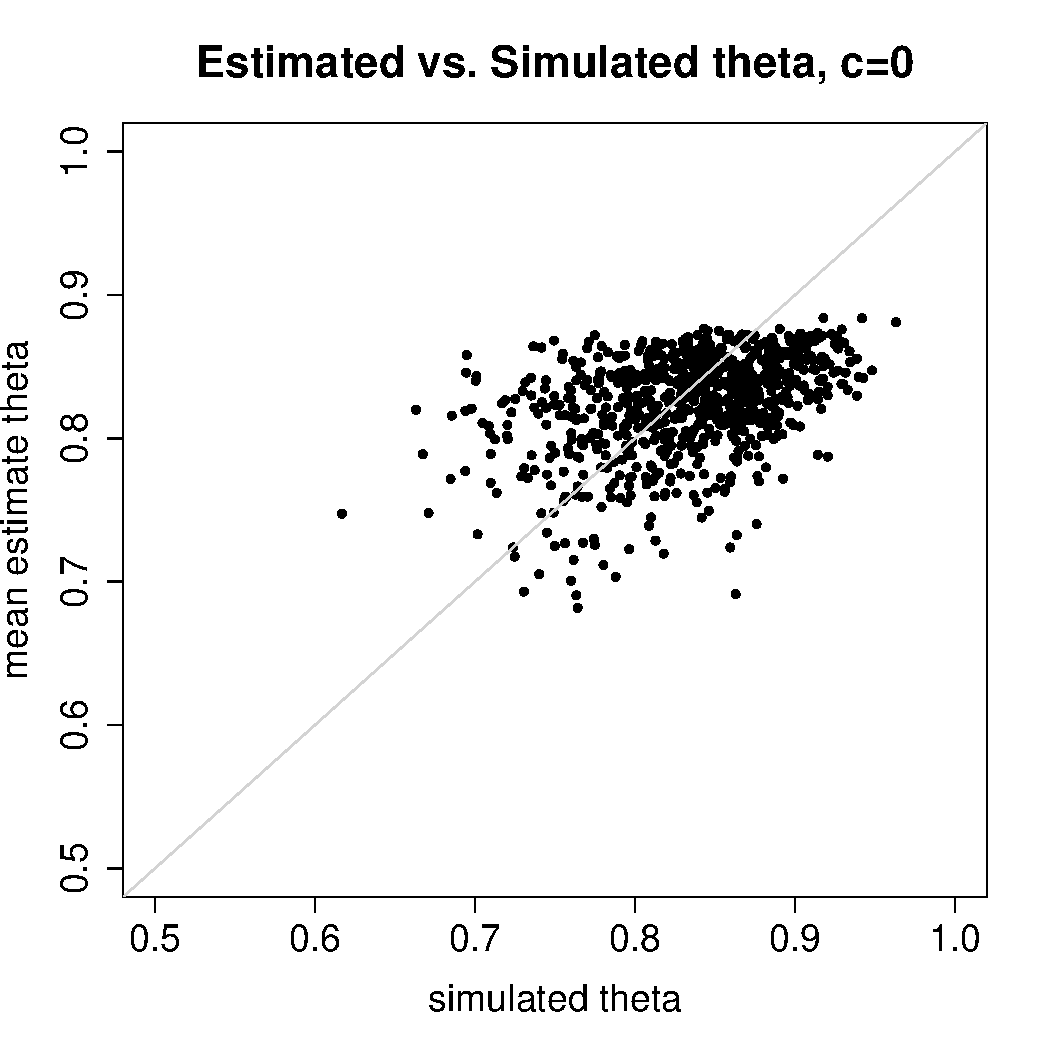
\includegraphics[width=0.4\textwidth]{pdf/beta-binomial-item-theta-0-fit.pdf}%
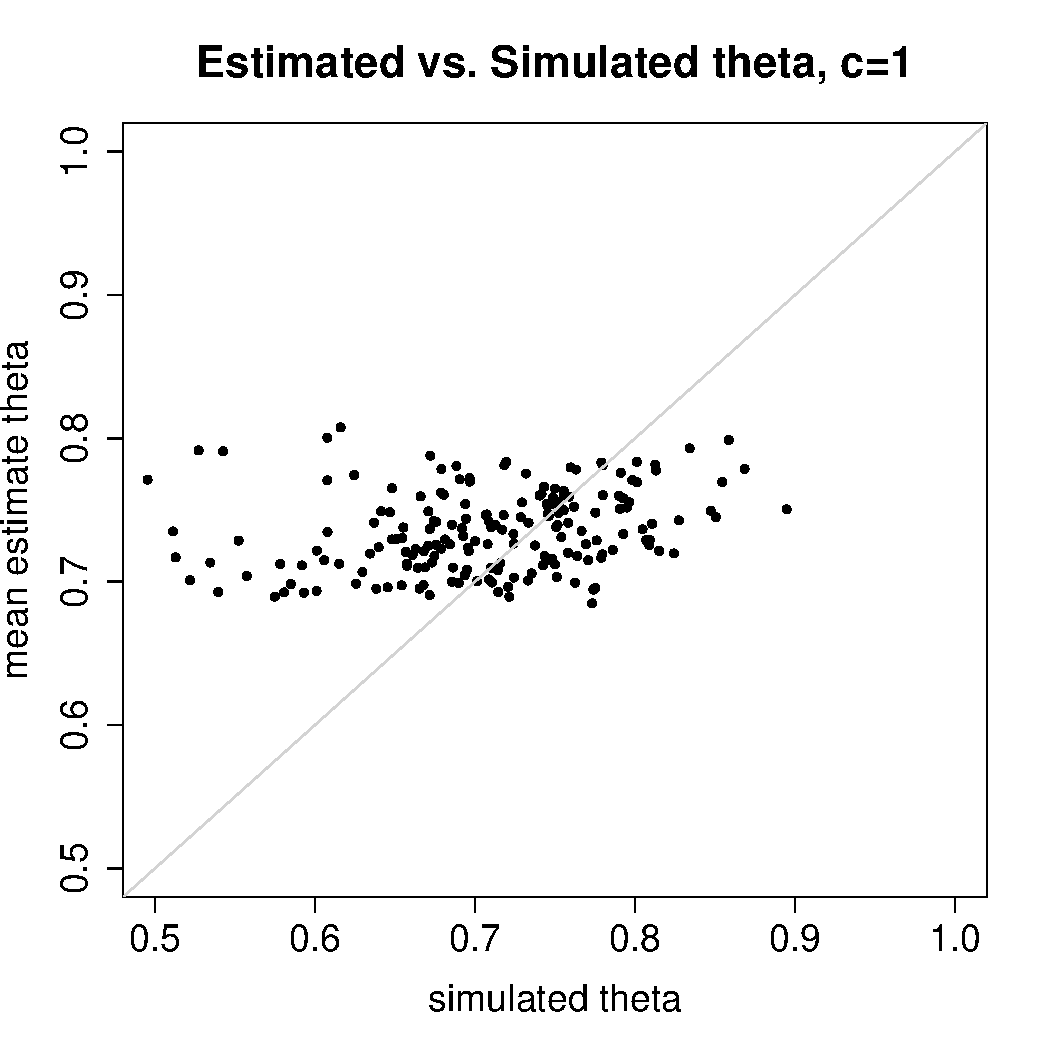
\includegraphics[width=0.4\textwidth]{pdf/beta-binomial-item-theta-1-fit.pdf}
\end{center}
\mycaption{Beta-binomial by item model: simulated versus mean estimated values
for $\theta_i$.  The two graphs represent $\theta_i$ drawn where the
true category $c_i = 0$ and where the true category $c_i = 1$.  This
shows the item-level parameters were not fit well at all in the
model.}%
\label{beta-binomial-item-theta-fits.fig}
\end{figure}
%
Because the $\theta$ values are drawn per item in this model, and
there are only an expected 10 annotators per item, a beta prior with a
scale of much greater than 10 will dominate the actual data.  This
Figure~\ref{beta-binomial-item-theta-fits.fig} reflects this behavior,
with fits broken down into one plot for simulated category 0 items and
one for simulated category 1 items.  Accurate estimates fall on the
diagonal, and almost no variation in estimate is seen between the
actual simulated values and the mean estimated values.  In other
words, the item-level parameters are not being well estimated with
only an expected 10 annotations per item.

\begin{figure}
\begin{center}
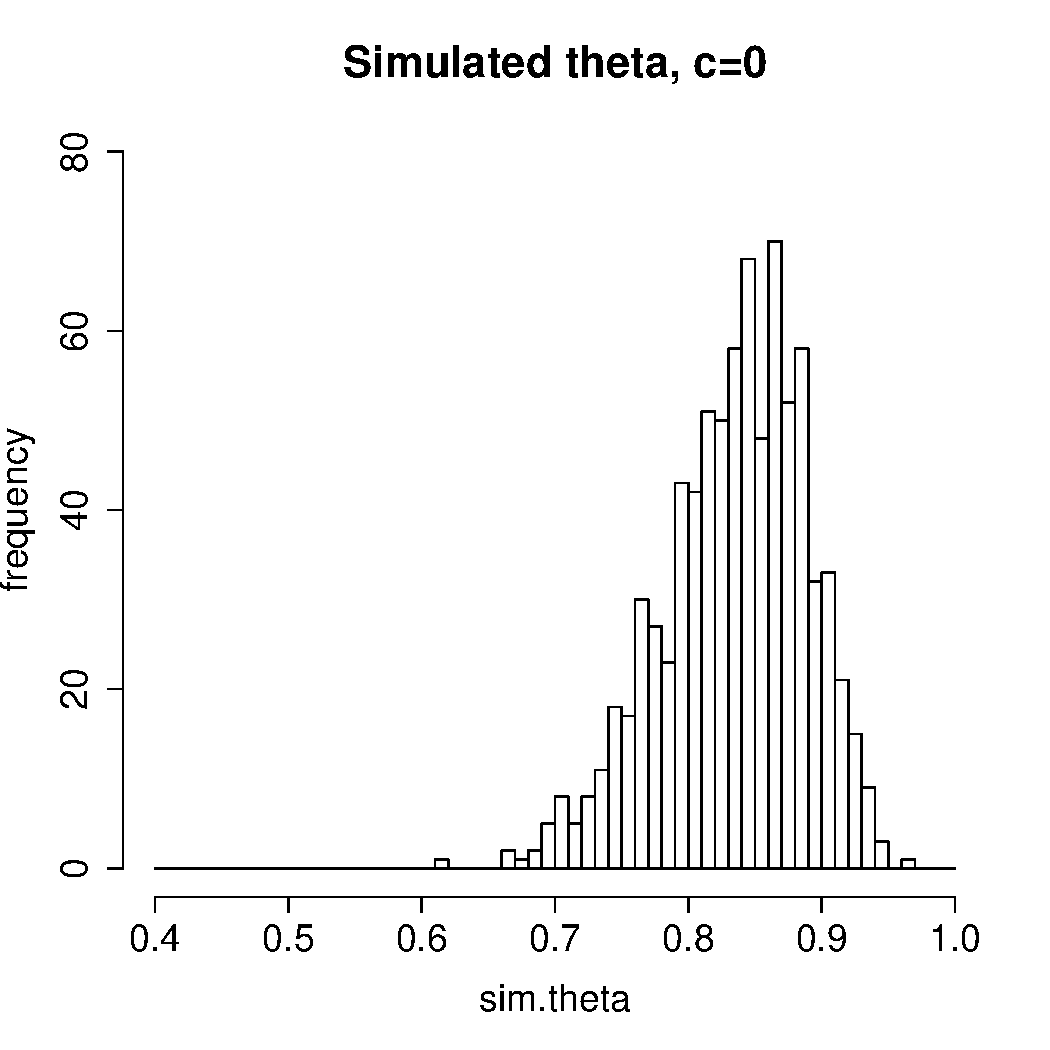
\includegraphics[width=0.4\textwidth]{pdf/beta-binomial-item-sim-theta-c0.pdf}%
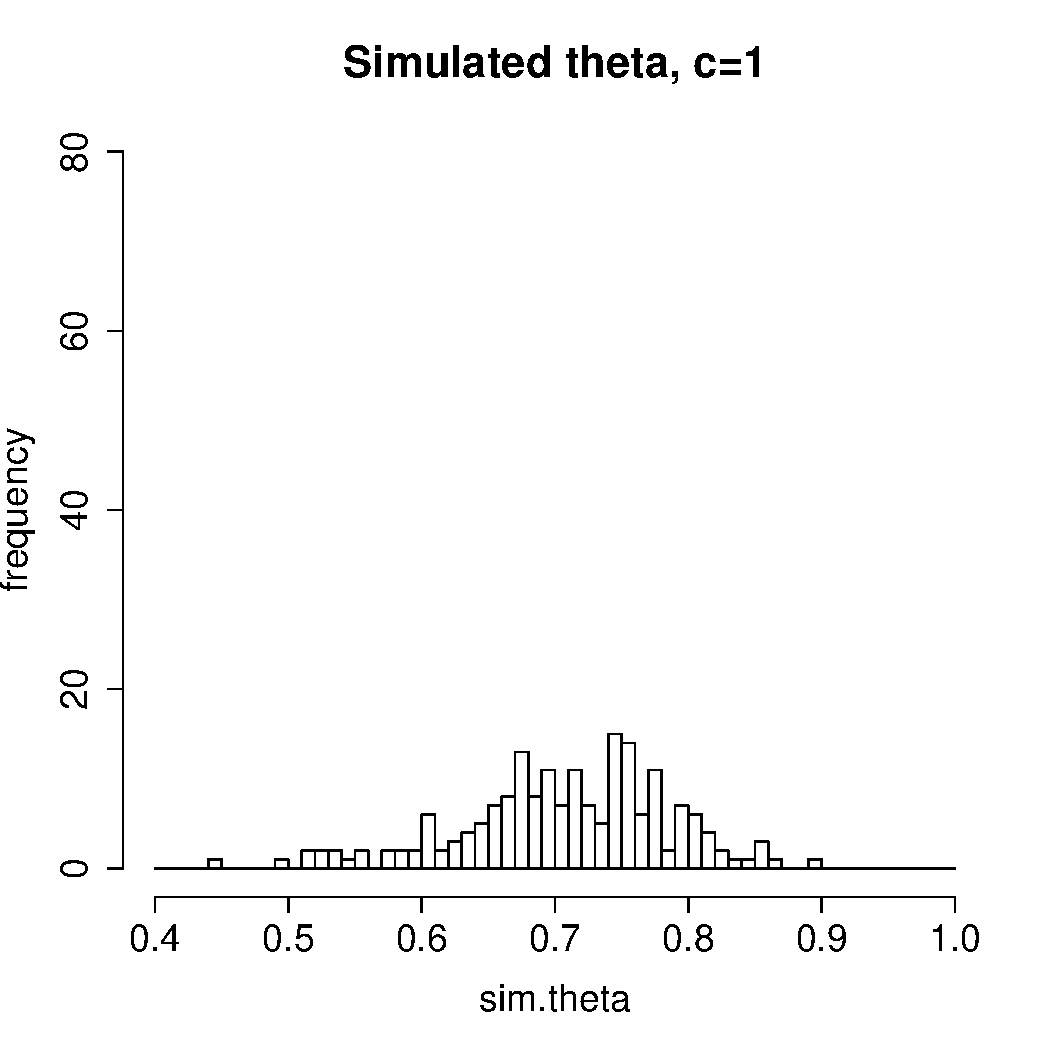
\includegraphics[width=0.4\textwidth]{pdf/beta-binomial-item-sim-theta-c1.pdf}
\end{center}
\mycaption{Beta-binomial by item model: histogram of simulated $\theta$ values
for category 0 and category 1 items.}%
\label{beta-binomial-item-sim-thetas.fig}
\end{figure}
%
The range of $\theta$ values drawn fro true category 0 and category 1
items are shown in Figure~\ref{beta-binomial-item-sim-thetas.fig}.
                         
\begin{figure}
\begin{center}
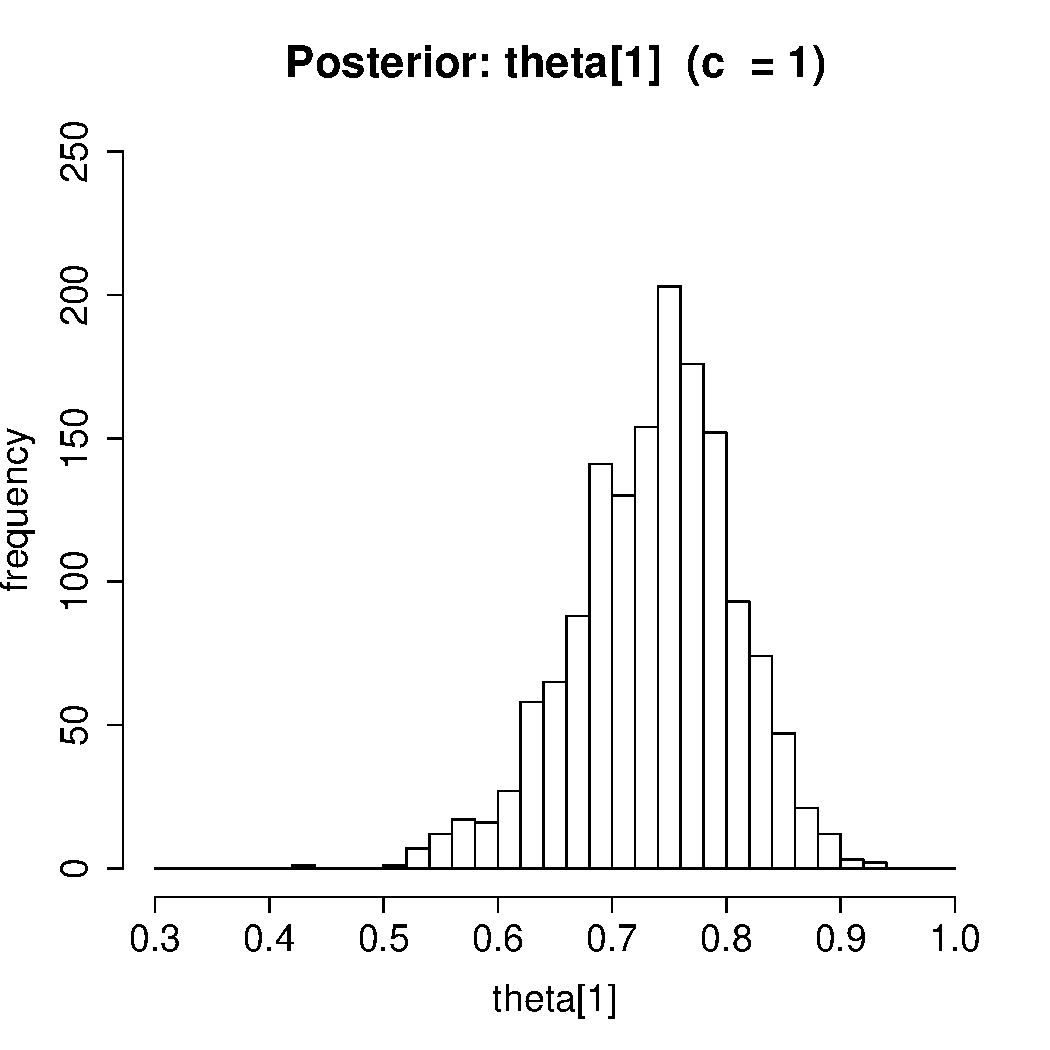
\includegraphics[width=0.4\textwidth]{pdf/beta-binomial-item-post-theta_1.pdf}%
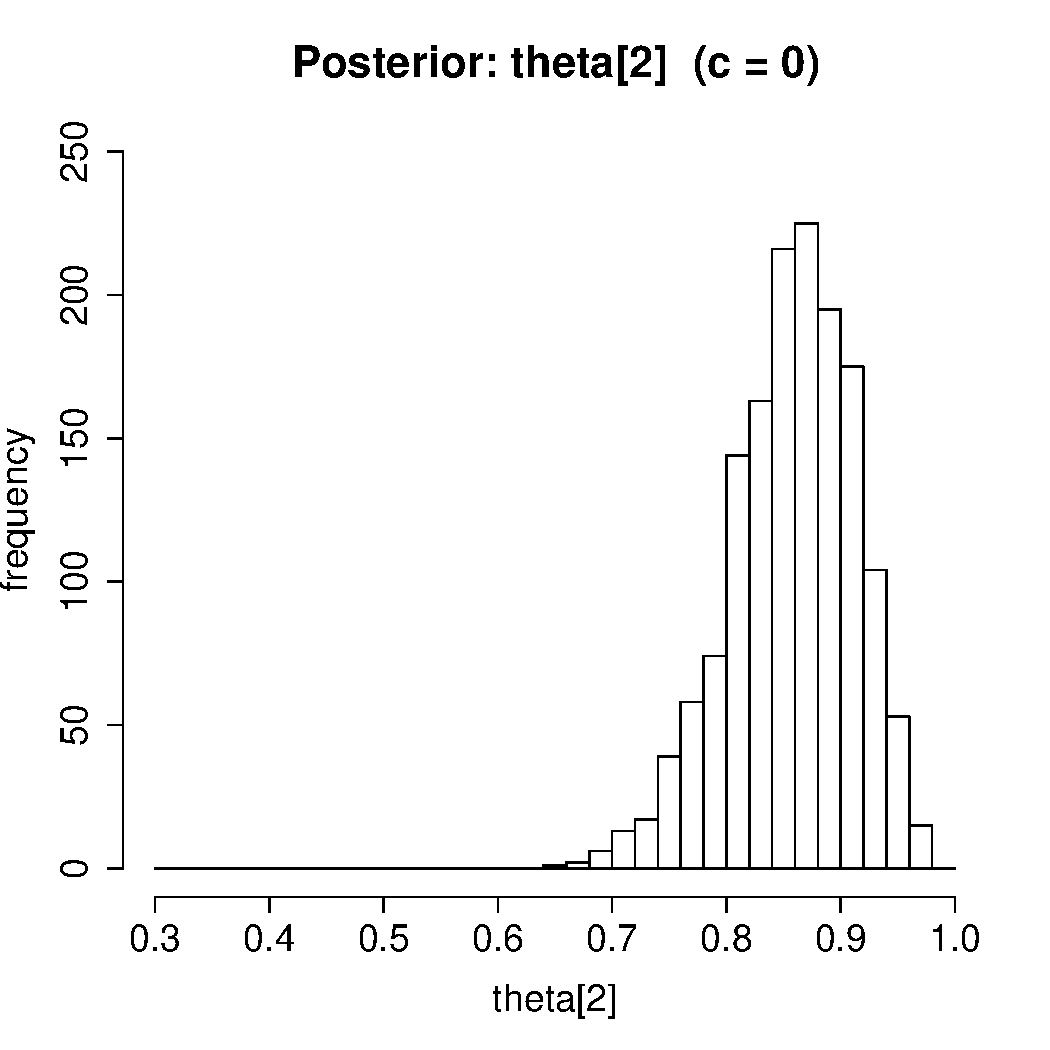
\includegraphics[width=0.4\textwidth]{pdf/beta-binomial-item-post-theta_2.pdf}
\end{center}
\mycaption{Beta-binomial by item model: histogram of posterior distribution
of estimated $\theta_1$ and $\theta_2$ values under the model.  In the
simulation, $c_1 = 1$ and $c_2=0$, $\theta_1=.80$ and $\theta_2=.79$,
and the annotations available were 100111111 and 0000000
respectively.}%
\label{beta-binomial-item-post-thetas.fig}
\end{figure}
%
The posterior uncertainty in item-level $\theta$ estimates is
reflected in the pair of posterior distribution estimates for
$\theta_1$ and $\theta_2$ in the simulated model, shown in
Figure~\ref{beta-binomial-item-post-thetas.fig}.  Most of the 95\%
posterior intervals are 0.2 to 0.3 wide.


\subsection{Simulated Logistic}

\begin{figure}
\begin{center}
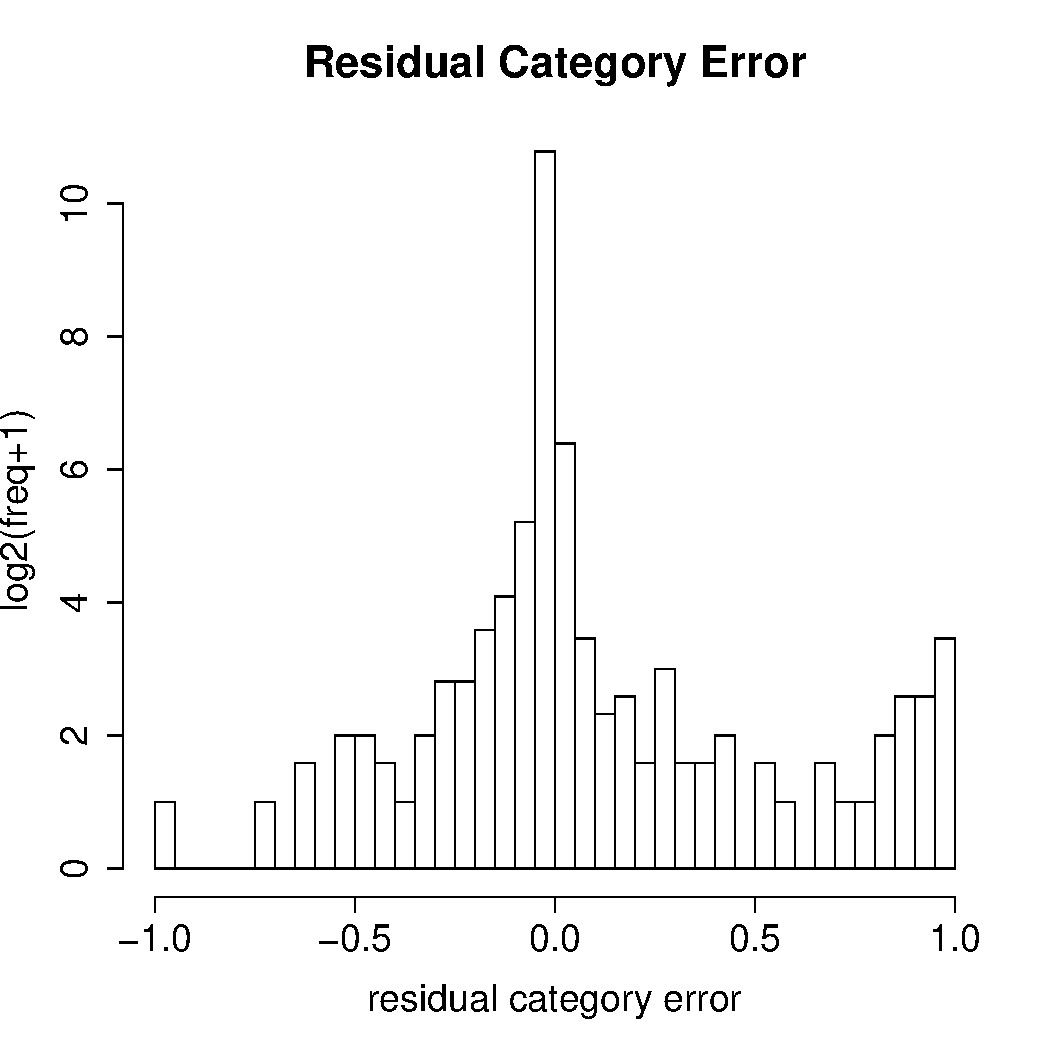
\includegraphics[width=0.4\textwidth]{pdf/logistic-cat-residual.pdf}%
\end{center}
\mycaption{Logistic model: histogram of residual category estimate
errors, consisting of the true category minus the mean posterior
category assignment.}%
\label{logistic-cat-residual.fig}
\end{figure}
%
Data simulated according to the logistic model fit surprisingly well
given that it includes both item-level and annotator-level effects, as
well as priors for both.  The logistic model didn't fare so well in
terms of residual category error, as shown in
Figure~\ref{logistic-cat-residual.fig}.  There are a total of 37
posterior errors in category assignment by most likely posterior
category.  The error curve is skewed, with the errors near 1.0
representing cases where the true category is 1 but the estimate is
near 0.

\begin{figure}
\begin{center}
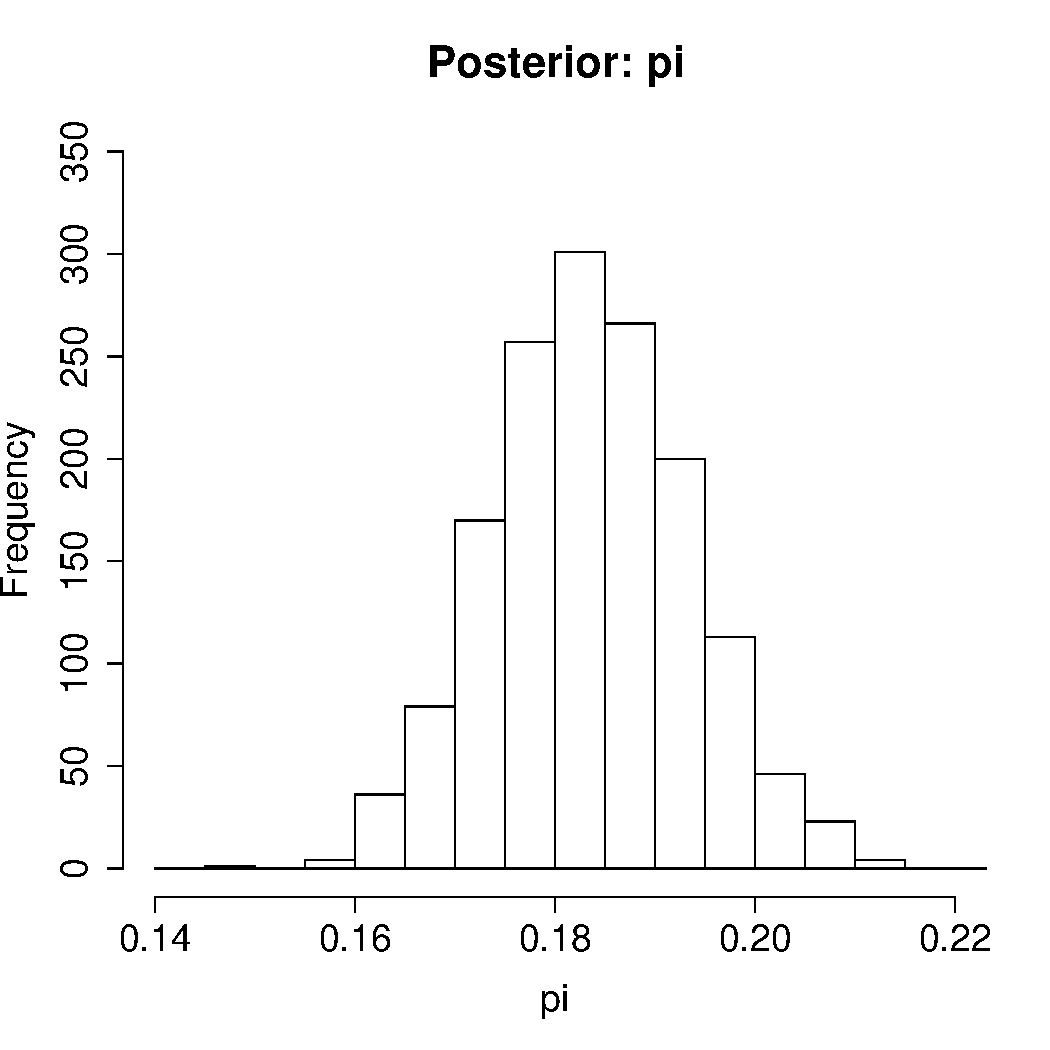
\includegraphics[width=0.4\textwidth]{pdf/logistic-posterior-pi.pdf}%
\end{center}
\mycaption{Logistic model: histogram of the posterior distribution
of the prevalence parameter $\pi$, where the simulated prevalence
was 0.2 and the sample prevalence was 0.189.}%
\label{logistic-posterior-pi.fig}
\end{figure}
%
Given the skew of the category error curve, it is perhaps not
surprising that the prevalence estimate is on the low side, with the
mean prevalence estimate at .184 versus a sample prevalence of .189.
The posterior prevalence histogram is in
Figure~\ref{logistic-posterior-pi.fig}.

\begin{figure}
\begin{center}
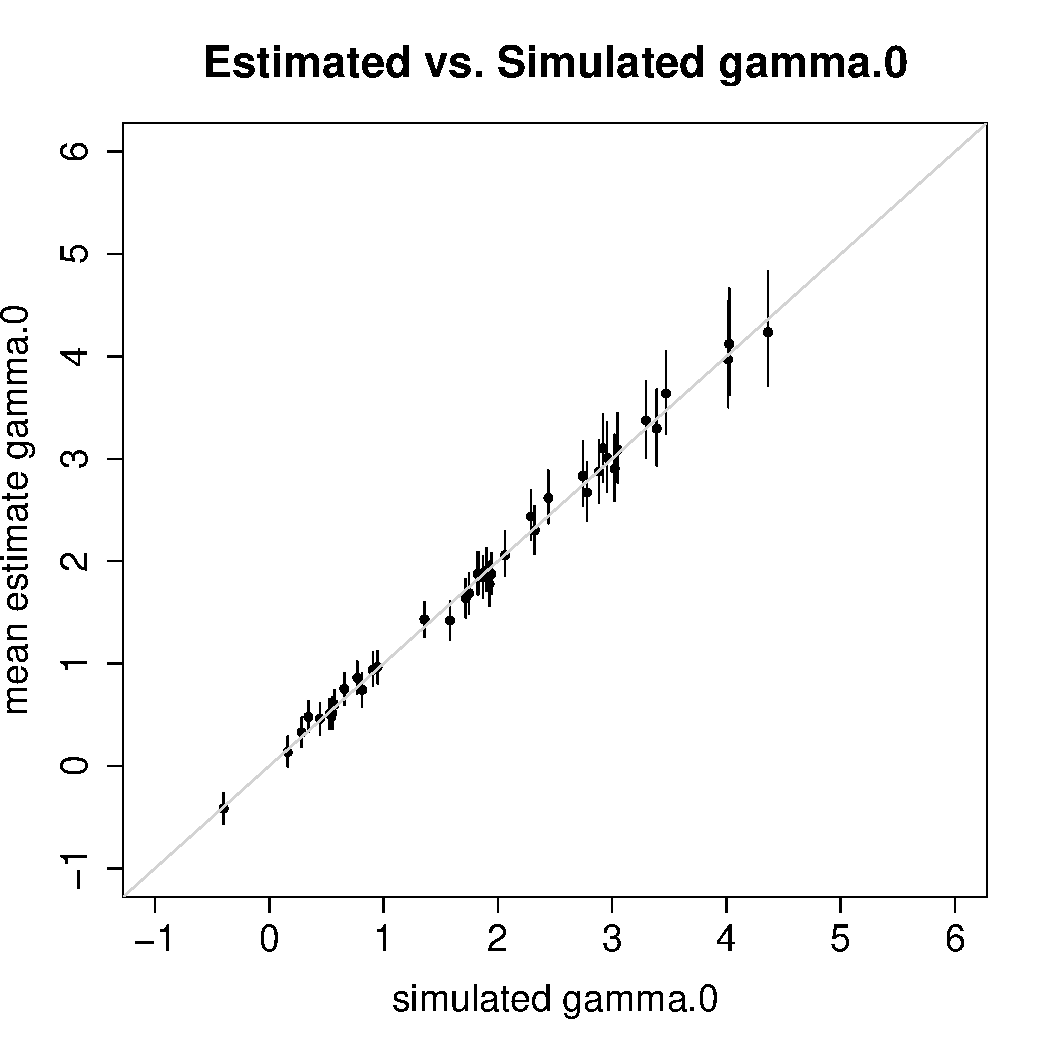
\includegraphics[width=0.4\textwidth]{pdf/logistic-gamma_0-fit.pdf}%
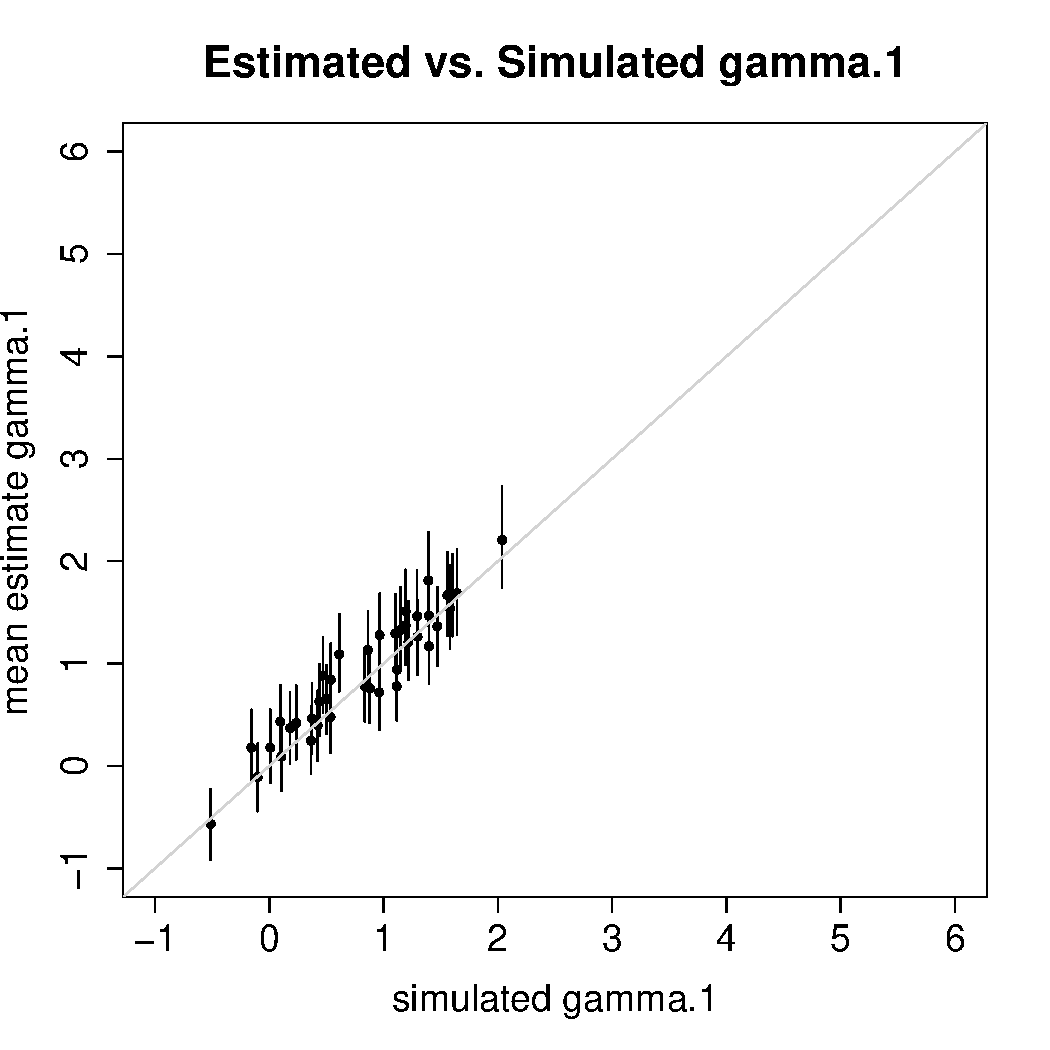
\includegraphics[width=0.4\textwidth]{pdf/logistic-gamma_1-fit.pdf}%
\end{center}
\mycaption{Logistic model: plot of simulated $\gamma_0$ and $\gamma_1$
values versus mean posterior values, along with 95\% posterior
intervals. The diagonal line represents a perfect fit.}%
\label{logistic-gammas-fit.fig}
\end{figure}
%
The annotator accuracy fits are shown in
Figure~\ref{logistic-gammas-fit.fig}.  These are all spot on, with the
$\gamma_0$ estimates having narrower posterior intervals due to four
times as much data for their estimation.

\begin{figure}
\begin{center}
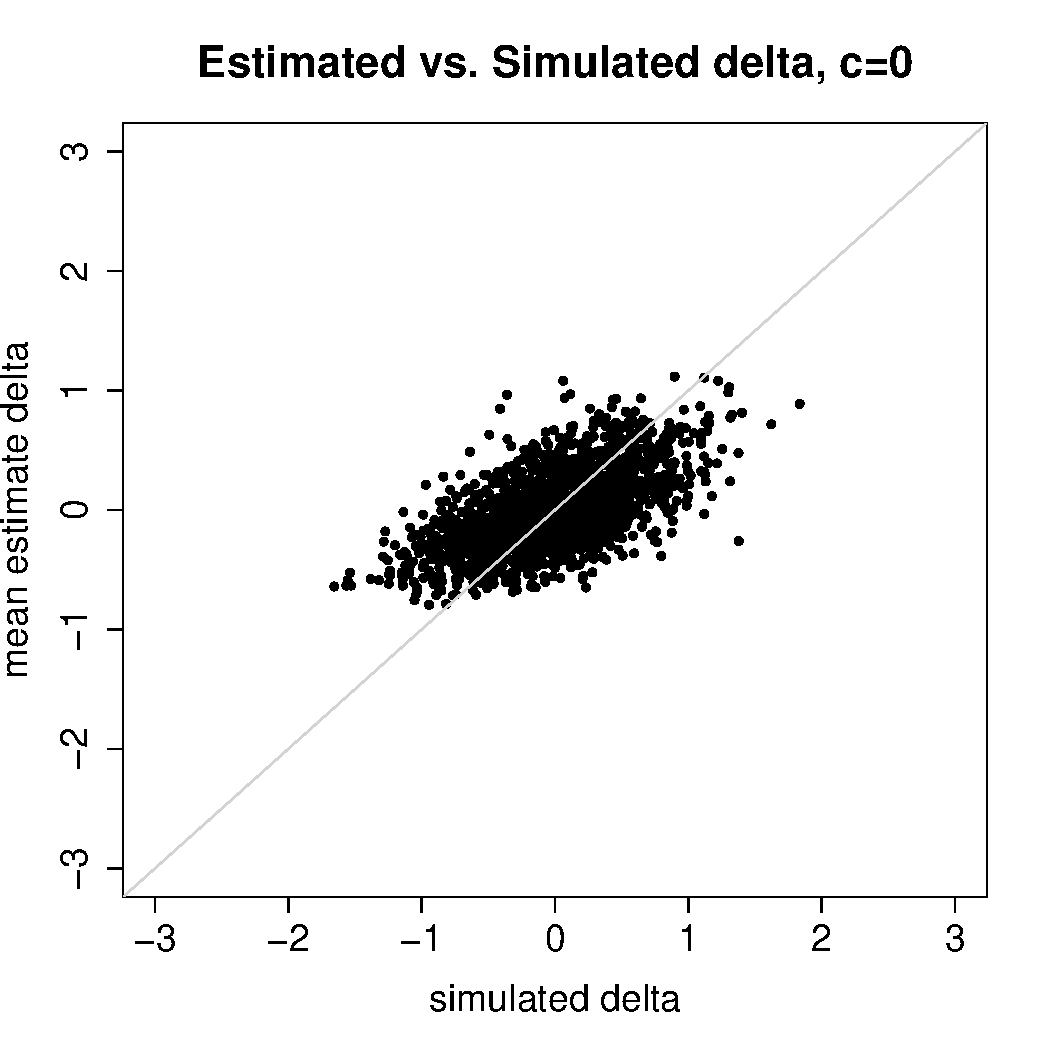
\includegraphics[width=0.4\textwidth]{pdf/logistic-delta_0-fit.pdf}%
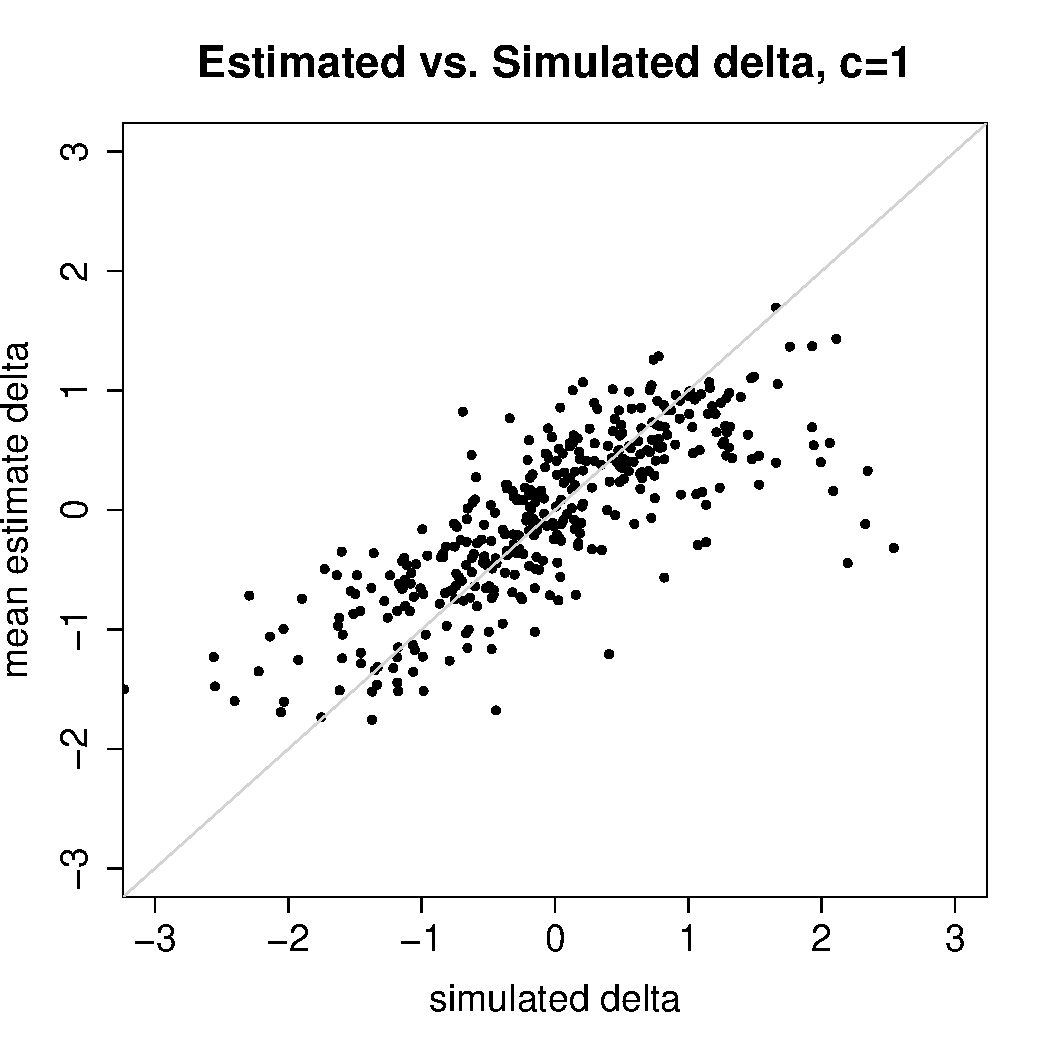
\includegraphics[width=0.4\textwidth]{pdf/logistic-delta_1-fit.pdf}%
\end{center}
\mycaption{Logistic model: plot of simulated $\delta$
values versus mean posterior values.  The two graphs represent
the cases where the true category $c_i = 0$ and $c_i = 1$ respectively.
The diagonal line represents a perfect fit.}%
\label{logistic-deltas-fit.fig}
\end{figure}
%
The item difficulty fits are shown in
Figure~\ref{logistic-deltas-fit.fig}.  Here, the $\delta$ values for
the category 1 items are estimated better than for the category 0
items.  Both fits are problematic in that there are only 10
annotations on average for each $\delta_i$ parameter estimated.  Here
the category 1 fits were much tighter, despite being based on fewer
data points.

\begin{figure}
\begin{center}
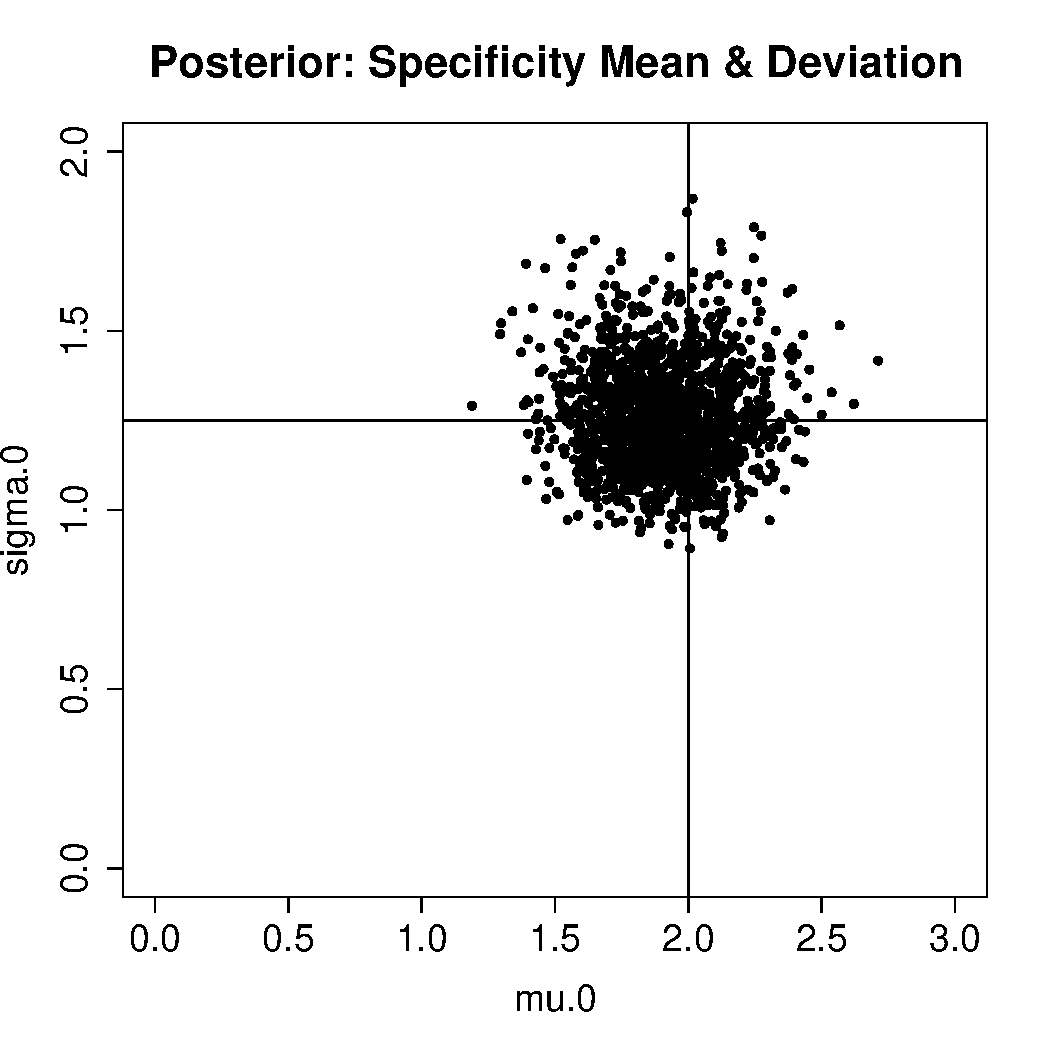
\includegraphics[width=0.4\textwidth]{pdf/logistic-scatter-spec.pdf}%
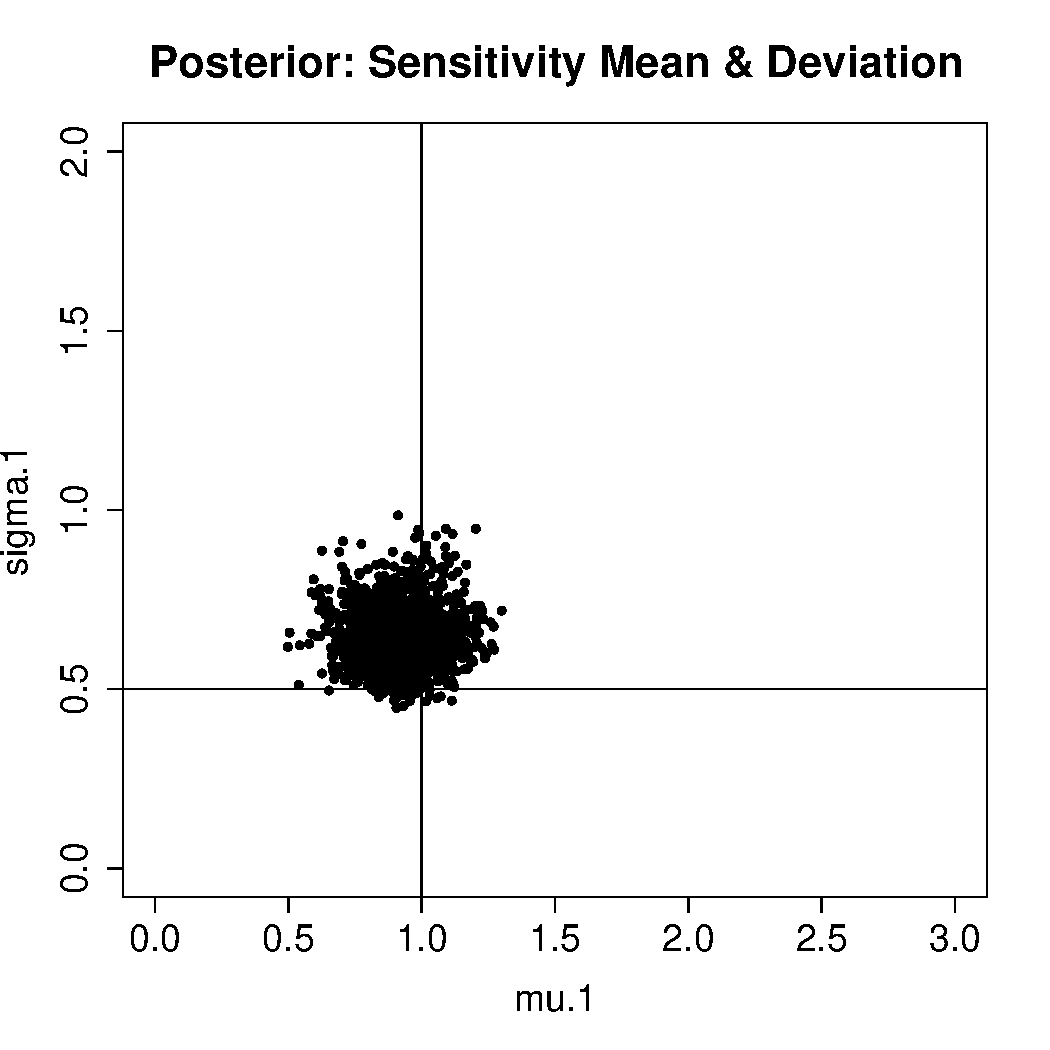
\includegraphics[width=0.4\textwidth]{pdf/logistic-scatter-sens.pdf}%
\end{center}
\mycaption{Logistic model: scatterplot of posterior samples of
annotator mean and variance parameters for category 0 (specificity)
and 1 (sensitivity) items respectively.  The horizontal and vertical
lines represent the simulated values from which the data being fit was
generated.  The sample means and variances from the simulated data
were $\mu_0 = 1.9$, $\sigma_0=1.25$ and $\mu_1 = .83$, $\sigma_1 =
.59$.}%
\label{logistic-scatters.fig}
\end{figure}
%
The multilevel parameters for annotator accuracy are shown in
Figure~\ref{logistic-scatters.fig}.  Here, the parameters fit better
for specificity mean $\mu_0$ and deviation $\sigma_0$, for which there
was four times as much data.  Both estimates are close to the sample
values.

\begin{figure}
\begin{center}
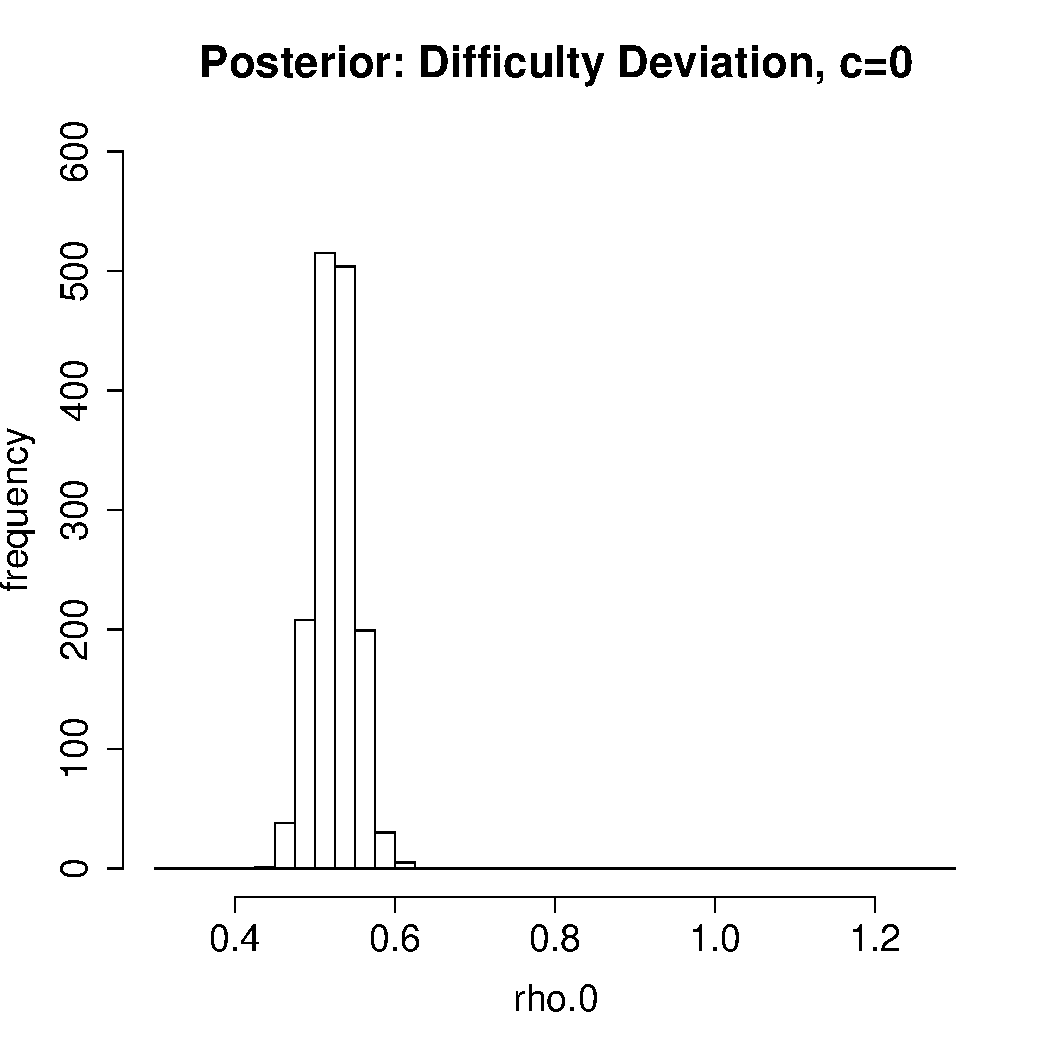
\includegraphics[width=0.4\textwidth]{pdf/logistic-post-rho_0.pdf}%
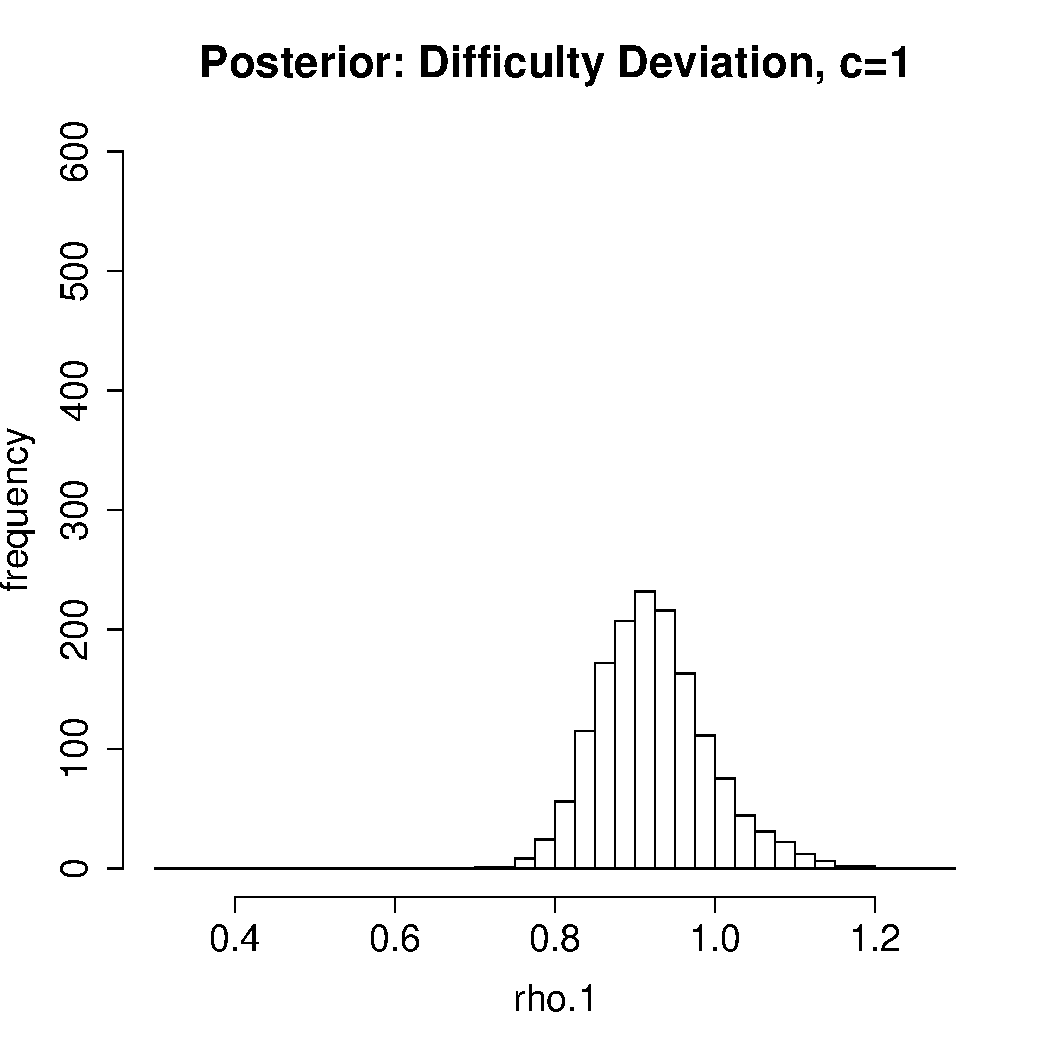
\includegraphics[width=0.4\textwidth]{pdf/logistic-post-rho_1.pdf}%
\end{center}
\mycaption{Logistic model: histogram of posterior samples of
the difficulty variance parameters for category 0 and 1
items.  The simulated values were $\rho_0 = 0.5$ and
$\rho_1=1.0$ with means fixed at zero.  The sample values
for category 0 items were mean -0.01 and $\rho_0 = 0.51$,
and for category 1 items were mean -0.03 and $\rho_1 = 0.97$.}%
\label{logistic-post-rhos.fig}
\end{figure}
%
The multilevel parameters for item difficulty
are shown in Figure~\ref{logistic-post-rhos.fig}.





\section{X-Ray Caries Diagnosis}

In this section and the next, we present analyses of real data sets.
Our multilevel models assume a degree of homogeneity among annotators
that is not present in many of the real epidemiological data sets,
because different types of tests such as physical inspection and blood
tests are applied.  Other data sets, such as Broemling's (2001)
thought-disorder data set have so few data annotators and items as to
make fitting a multilevel Bayesian model quixotic at best.

Espeland and Handelman~(1989) collected the diagnoses of 5 dentists
over 3869 X-rays for caries, a kind of pre-cavity.  The data was
also analyzed in Albert and Dodd~(2004).  The study involved a fixed
panel design in which every dentist annotated every X-ray.  A fixed panel
designs with dichotomous data and a limited number of annotators is
easily summarized in the form of a contingency table, which reports
counts for every possible response. The dentistry data is presented
as such in Figure~\ref{caries-data.fig}.

\begin{figure}
\begin{center}
\begin{tabular}{cr|cr}
{\it Dentists} & {\it Count} &
{\it Dentists} & {\it Count}
\\ \hline
00000 & 1880 & 10000 & 22 \\
00001 & 789 & 10001 & 26 \\
00010 & 43 & 10010 & 6 \\
00011 & 75 & 10011 & 14 \\
00100 & 23 & 10100 & 1 \\
00101 & 63 & 10101 & 20 \\
00110 & 8 & 10110 & 2 \\
00111 & 22 & 10111 & 17 \\
01000 & 188 & 11000 & 2 \\
01001 & 191 & 11001 & 20 \\
01010 & 17 & 11010 & 6 \\
01011 & 67 & 11011 & 27 \\
01100 & 15 & 11100 & 3 \\
01101 & 85 & 11101 & 72 \\
01110 & 8 & 11110 & 1 \\
01111 & 56 & 11111 & 100
\end{tabular}
\end{center}
\mycaption{X-Ray caries diagnosis contingency table.  Five dentists' annotations
for 3869 X-rays for the presence of caries (a kind of pre-cavity).
For example, there were 43 X-rays for which dentists 1, 2, 3 and 5 said
there was no caries but dentist 4 said there was caries.  There was
one X-ray for which dentists 1-4 said there was caries, but dentist 5
said there wasn't.}%
\label{caries-data.fig}
\end{figure}

Rather than presenting full posterior histograms or scatterplots, we
will present summaries of model fits for real data sets through
posterior quantiles, including medians, 50\% and 95\% intervals.

\subsection{Binomial Model Fit}

The model had $\hat{R}$ values for the
following parameters very near 1; some of the category $\hat{R}$
values were between 1 and 1.5.  The quantiles for the posterior
binomial parameters are:
%
\begin{center}
\begin{tabular}{c|rrrrr}
            & \multicolumn{5}{c}{{\it Quantiles}} \\
{\it Param} & .025 & .250 & .500 & .750 & .975 \\ \hline
$\pi$       & .15 & .16 & .17 & .17 & .19 \\
$\theta_0$  & .89 & .89 & .89 & .90 & .90 \\
$\theta_1$  & .62 & .64 & .66 & .67 & .69 \\
\end{tabular}
\end{center}
%

\subsection{Beta-Binomial by Annotator Fit}

All values for parameters other
than categories fit with $\hat{R}$ near 1.0; some values for $c$ had
$\hat{R}$ values between 1 and 1.5.  The quantiles for the
posterior beta-binomial by annotator model parameters are:
%
\begin{center}
\begin{tabular}{c|rrrrr}
            & \multicolumn{5}{c}{{\it Quantiles}} \\
{\it Param} & .025 & .250 & .500 & .750 & .975 \\ \hline
$\pi$       & .18 & .19 & .20 & .20 & .21 \\
$\alpha_0/(\alpha_0 + \beta_0)$  & .58 & .75 & .82 & .87 & .93 \\
$\alpha_0 + \beta_0$           & 1.0 & 1.4 & 2.1 & 3.4 & 8.6 \\
$\alpha_1/(\alpha_1 + \beta_1)$  & .37 & .53 & .60 & .67 & .79 \\
$\alpha_1 + \beta_1$           & 1.1 & 1.7 & 2.6 & 4.0 & 9.1 \\
\end{tabular}
\end{center}
%
Both models estimate prevalence, but the estimate is much higher
for the beta-binomial by annotator model.

\begin{figure}
\begin{center}
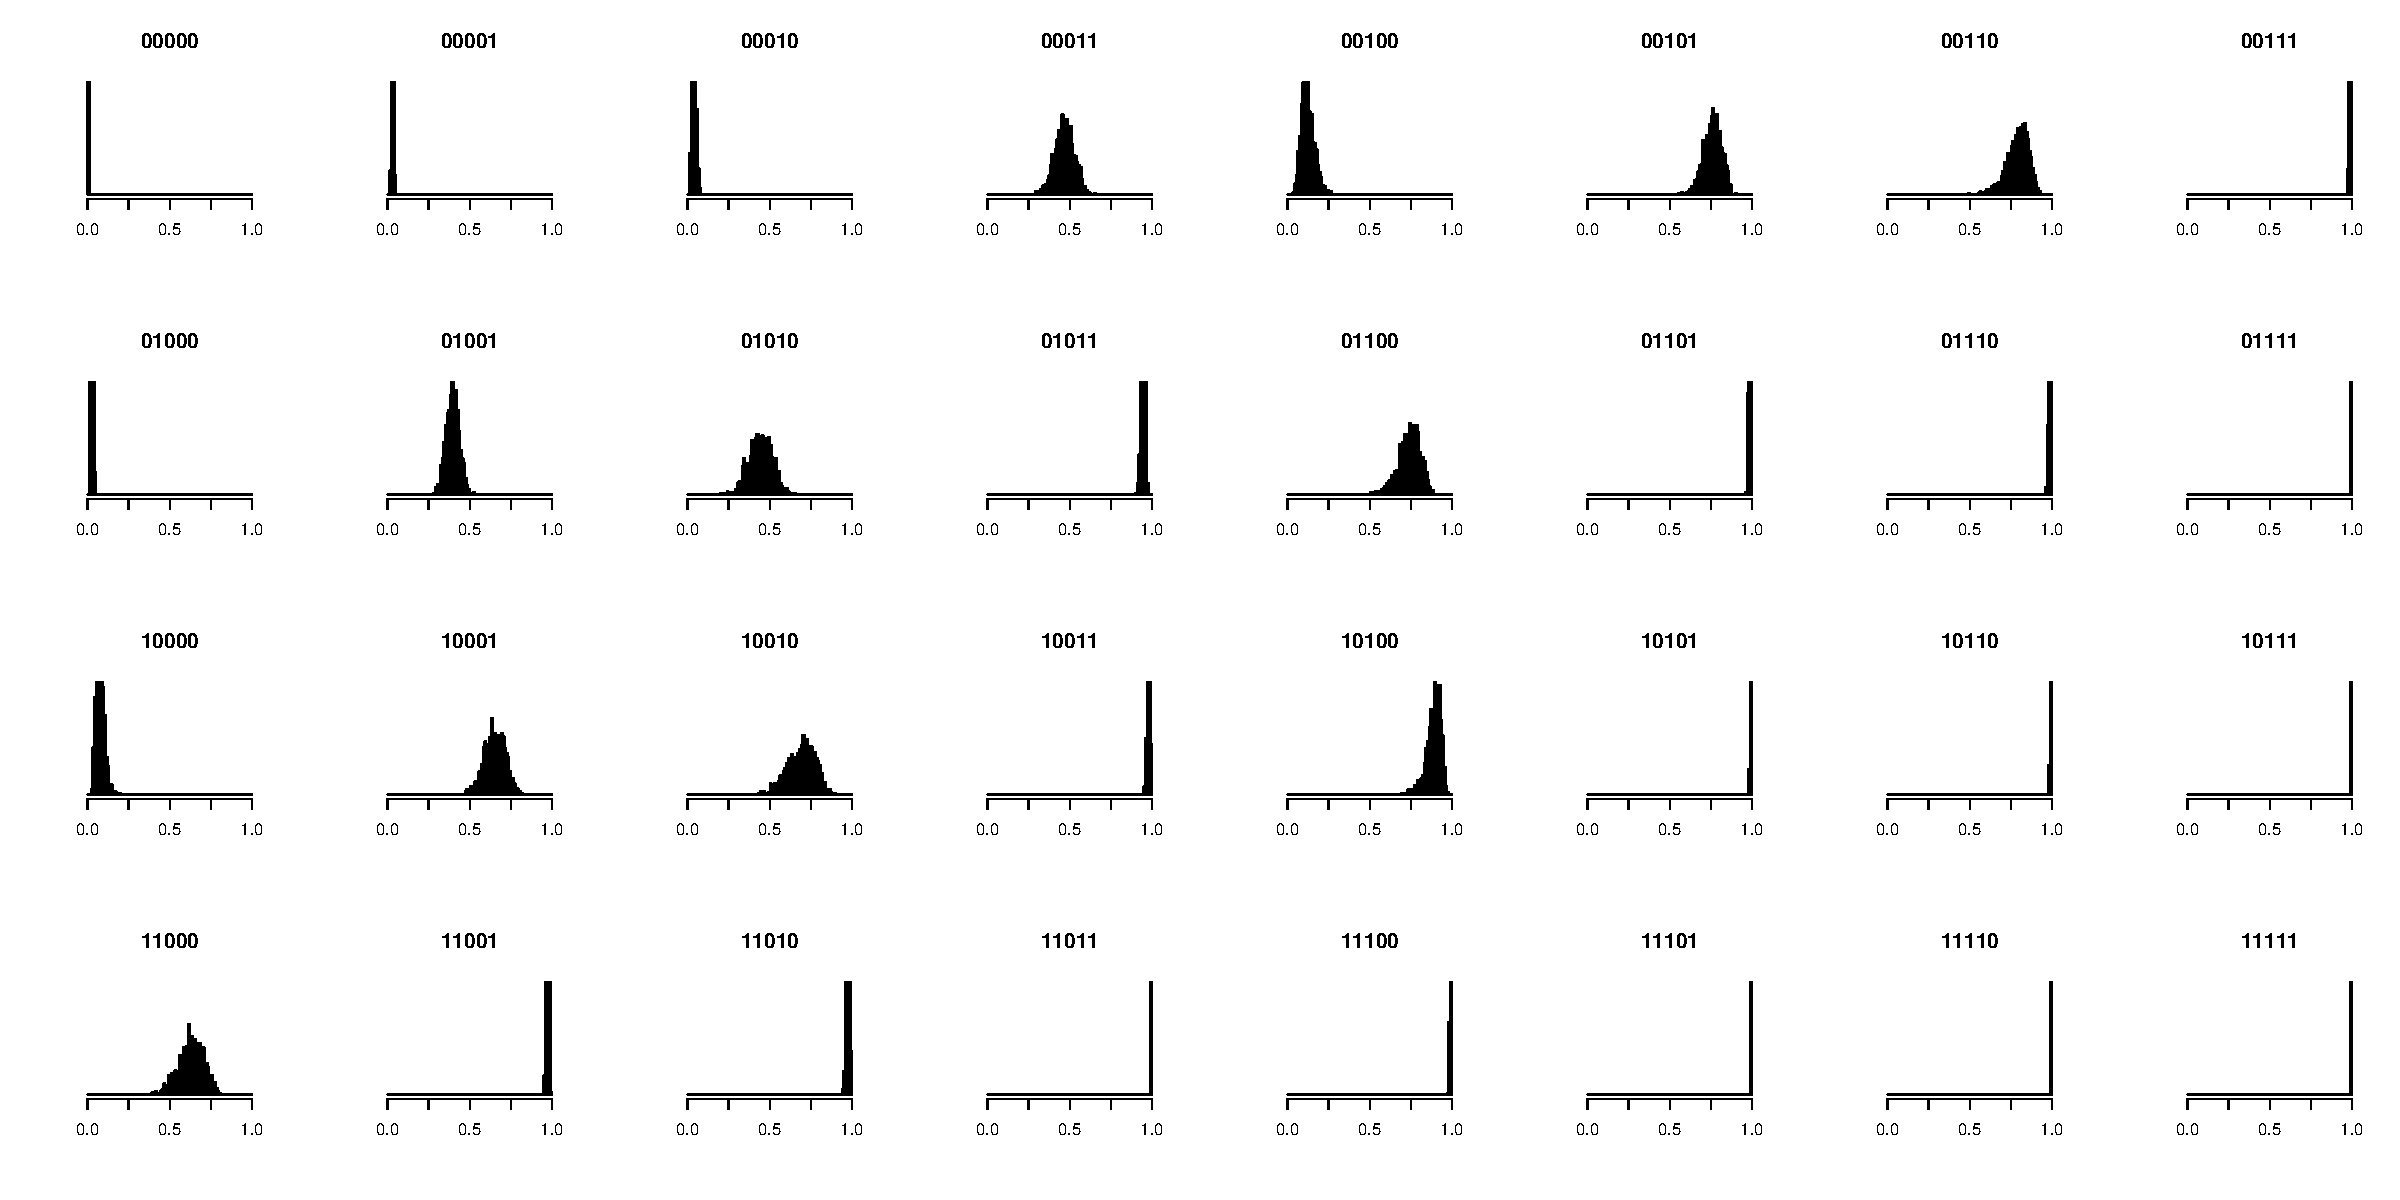
\includegraphics[width=\textwidth]{pdf/dentistry-beta-binomial-anno-post-cats.pdf}
\end{center}
\mycaption{Dentistry data under beta-binomial by annotator: 
posterior category histograms drawn to the same horizontal and
vertical scale.}%
\label{dentistry-beta-binomial-anno-post-cats.fig}
\end{figure}
%
In Figure~\ref{dentistry-beta-binomial-anno-post-cats.fig} we display
the posterior category distributions for the beta-binomial by
annotator model in the form of histograms for all 32 patterns of
annotator responses (note that the highly skewed distributions are
clipped on their top end, which is why not all histograms have the
same volume).

\begin{figure}
\begin{center}
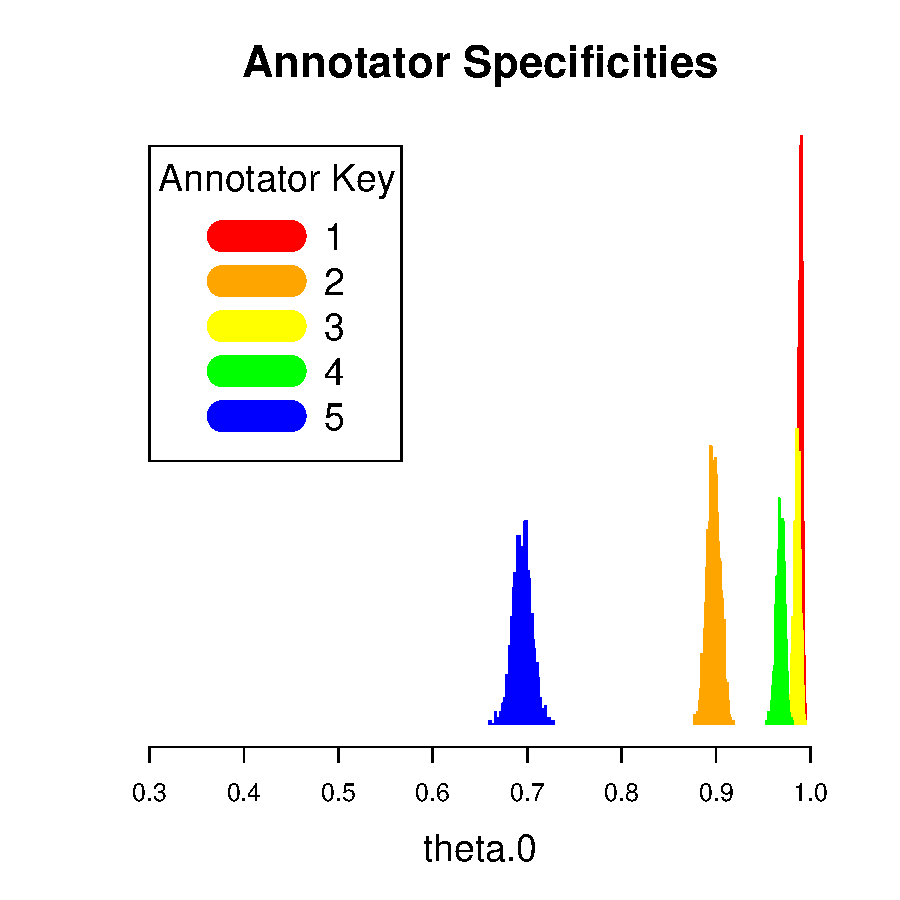
\includegraphics[width=0.4\textwidth]{pdf/dentistry-theta_0-hist.pdf}%
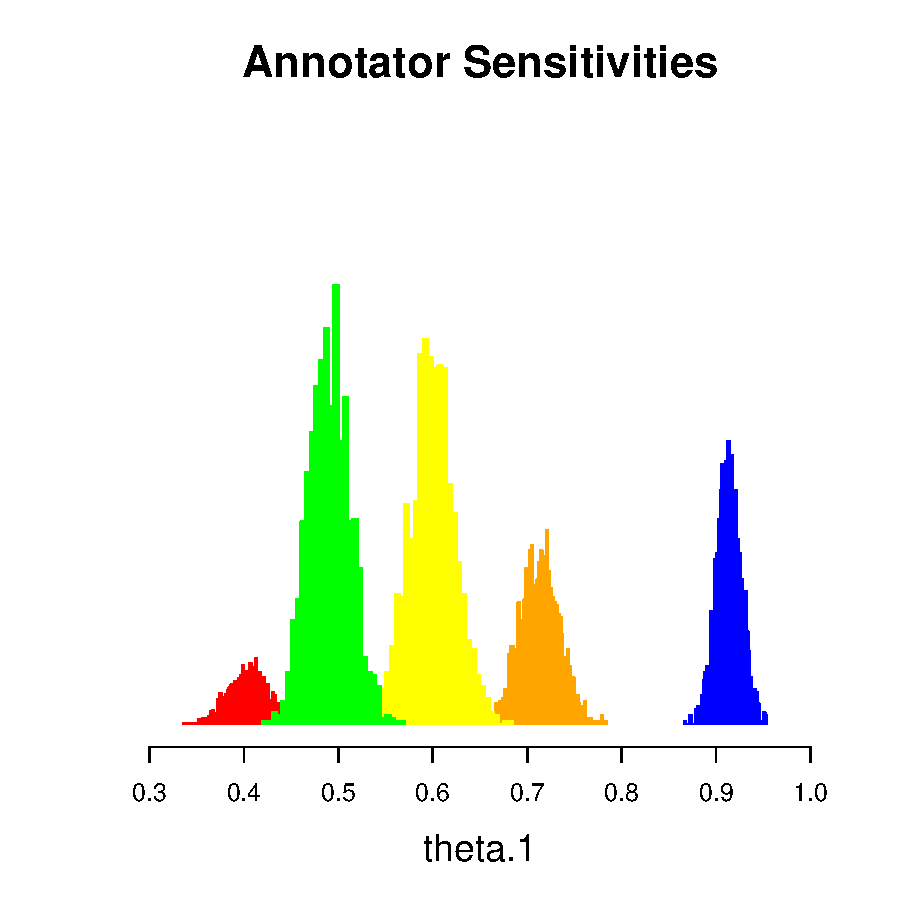
\includegraphics[width=0.4\textwidth]{pdf/dentistry-theta_1-hist.pdf}
\end{center}
\mycaption{Dentistry data under beta-binomial by annotator: posterior
annotator specificity and sensitivity histograms.}%
\label{dentistry-beta-binomial-anno-post-annos.fig}
\end{figure}
%
In Figure~\ref{dentistry-beta-binomial-anno-post-annos.fig} we display
the posterior distribution of annotator specificity and sensitivty
parameters.  This figure clearly illustrates that the performance on
category 0 items is worse than on category 1 items.  It also shows the
bias of annotators, with annotator 1 strongly favoring category 0 and
annotator 5 strongly favoring category 1.  Additionally, annotator 3
can be seen to have better sensitivity and specificity than annotator
4.


\subsection{Beta-Binomial by Item Fit}

The beta-binomial by item model is
the most problematic to fit.  There doesn't seem to be enough data to
estimate the scale parameters of the beta priors for accuracies for
category 0 and category 1 items, and the posterior variation on the
$\theta_i$ (by item) parameters is typically very wide.  We actually
ran 2000 iterations after which point the $\hat{R}$ values for
prevalence and the per-item $\theta_i$ values were all near 1.  The
$\hat{R}$ values for the beta priors were all under 1.25, but the
chains continued to explore large values for the beta scale
parameters.  The quantiles for the posteriors for the parameters of
interest for the beta-binomial by item model are:
%
\begin{center}
\begin{tabular}{c|rrrrr}
            & \multicolumn{5}{c}{{\it Quantiles}} \\
{\it Param} & .025 & .250 & .500 & .750 & .975 \\ \hline
$\pi$       & .11 & .13 & .13 & .14 & .15 \\
$\alpha_0/(\alpha_0 + \beta_0)$  & .87 & .88 & .88 & .88 & .89 \\
$\alpha_0 + \beta_0$           & 15 & 18 & 21 & 24 & 35 \\
$\alpha_1/(\alpha_1 + \beta_1)$  & .67 & .69 & .70 & .71 & .73 \\
$\alpha_1 + \beta_1$           & 39 & 54 & 72 & 105 & 217 \\
\end{tabular}
\end{center}
%
Given the extreme variation visible through inspection of the data,
the beta-binomial by item model is implausible.  So its low estimates
of prevalence should not be taken too seriously.


\subsection{Logistic Fit}

Just as in the beta-binomial by item model, five annotators per item
are simply too few to tightly estimate item difficulty.  As a result,
the posterior deviation parameters were estimated with 95\% posterior
intervals for $\rho_0$ of (.13,.31) and for $\rho_1$ of (.24,.35),
which means most difficulties were estimated near 0.

Like the beta-binomial by annotator model, the median
posterior prevalence is 0.197, which is the sample mean of the design
matrix $x$.  That is, 0.197 of all annotations by all annotators of
all items were category 1, and 0.803 were category 0.

As we show in the next section, Bayesian predictive inference, which
averages over the uncertainty in the difficulty estimates, shows
little effect of problem difficulty.  Only when the group-level
deviation parameters $\rho_0$ and $\rho_1$ are fixed to be greater
than 1 will the overdispersion effect of item difficulty begin to
assert itself.

Because of the limited ability to estimate item effects, posterior
intervals for annotator sensitivity and specificity looked very much
like those for the beta-binomial model when translated from the
logistic scale.


\subsection{Posterior Predictive Inference}

A standard way to evaluate the posterior fit of models such as these
is to look at the marginal predictions of the counts in the
contingency table.  We provide Bayesian posteriors for this value for
all four models.  The result is shown in
Figure~\ref{dentistry-contingency-fit.fig}.
%
\begin{figure}
\begin{center}
\footnotesize
\begin{tabular}{cr|rrrrr}
& & \multicolumn{4}{c}{{\it Model Prediction Quantiles} (0.025,0.5,0.975)} \\
{\it Labels} & {\it Freq} & {\it Binom} & {\it Binom by Anno} & {\it Binom by
Item} & {\it Logistic} & {\it Logistic$^*$} \\ \hline
00000 &  1880 & (1794,1854,1914) & (1774,1836,1896) & (1818,1877,1935)  & (1758,1836,1916) & (1723,1812,1899) \\
00001 &  789 & (214,223,232)  & (779,829,880) & (206,214,223)  & (758,830,892) & (724,788,864) \\
00010 &  43 & (214,223,232) & (49,62,79) & (206,214,223)  & (40,62,86) & (40,59,78) \\
00011 &  75 & (35,37,39) & (43,50,57) & (39,41,43)  & (34,50,68) & (50,67,90) \\
00100 &  23 & (214,223,232) & (19,29,41) &  (206,214,223)  & (16,29,45) & (17,29,45) \\
00101 &  63 & (35,37,39) & (40,47,55) & (39,41,43)  & (34,48,66) & (41,54,75) \\
00110 &  8  & (35,37,39) & (3.1,4.1,5.4) & (39,41,43)  & (1,4,8.5) & (1,4,9.5) \\
00111 &  22 & (22,25,27) & (28,35,42) & (21,23,25)  & (21,34,48) & (15,26,39) \\
01000 &  188 & (214,223,232) &  (190,215,242) & (206,214,223)  & (176,210,248) & (164,197,233) \\
01001 &  191 & (35,37,39) &   (138,152,166) & (39,41,43)  & (130,156,185) & (182,214,248) \\
01010 &  17  & (35,37,39) &  (10,12,15) & (39,41,43)  & (6,12,21) & (9,16,26) \\
01011 &  67  & (22,25,27) &   (51,61,72) & (21,23,25)  & (41,58,80) & (42,58,75) \\
01100 &  15  & (35,37,39) & (8.9,11,14) & (39,41,43)  & (5,12,21) & (7,13,21) \\
01101 &  85  & (22,25,27) & (78,91,106) & (21,23,25)  & (67,90,111) & (56,75,94) \\
01110 &  8  & (22,25,27) & (5.7,8.3,11) & (21,23,25)  & (3,7,15) & (2,7,13) \\
01111 &  56 & (38,41,45) & (75,86,99) & (35,39,42)  & (63,68,109) & (62,79,100) \\
10000 &  22 & (214,223,232) &  (14,21,31) & (206,214,223)  & (12,21,34) & (12,20,34) \\
10001 &  26 & (35,37,39) &  (21,25,30) & (39,41,43)  & (16,25,37) & (19,31,41) \\
10010 &  6  & (35,37,39) &  (1.6,2.1,2.8) & (39,41,43)  & (0,2,5.5) & (0,2,5) \\
10011 &  14 & (22,25,27) &  (12,16,20) & (21,23,25)  & (8,15,23) & (6,12,20) \\
10100 &  1  & (35,37,39) &  (1.8,2.6,3.5) & (39,41,43)  & (0,3,6) & (0,2,7) \\
10101 &  20  & (22,25,27) &   (20,24,30) & (21,23,25)  & (14,23,37) & (9.5,19,28) \\
10110 &  2  & (22,25,27) &  (1.5,2.2,3.2) & (21,23,25)  & (0,2,6) & (0,2,5) \\
10111 &  17  & (38,41,45) & (19,23,29) & (35,39,42)  & (14,22,33) & (11,20,30)\\
11000 &  2  & (35,37,39) &  (4.7,6.1,7.7) & (39,41,43)  & (2,6,12) & (3,7,14) \\
11001 &  20  & (22,25,27) &  (34,42,50) & (21,23,25)  & (28,41,55) & (25,35,48) \\
11010 &  6  & (22,25,27) &  (2.6,3.8,5.2) & (21,23,25)  & (0,3,8) & (0,3,7) \\
11011 &  27 & (38,41,45) &   (32,39,47) & (35,39,42)  & (25,38,53) & (22,34,50) \\
11100 &  3  & (22,25,27) &  (4,5.8,7.8) & (21,23,25)  & (1,6,11) & (1,4,9) \\
11101 &  72  & (38,41,45) &  (51,61,71) & (35,39,42)  & (46,61,78) & (39,55,74) \\
11110 &  1  & (38,41,45) &  (3.8,5.5,7.5) & (35,39,42)  & (2,5,11) & (1,5,10) \\
11111 &  100 & (64,78,93) & (49,59,70) & (80,93,109)  & (44,63,83) & (86,106,132) \\
\hline
$\pi$ & unk & (.15,.17,.19) & (.18,.20,.21) & (.12,.13,.15) & (.18,.19,.21) & (.18,.20,.22) \\ \hline
$X^2$  &      & 3177 & 131 & 3196 & 114 & 59 \\
\end{tabular}
\end{center}
\mycaption{Dentistry model fit: observed and posterior predictive
estimates of outcome counts.  Predictive estimates are in the form of
model quantiles including the median and 95\% intervals.  The last
logistic column marked with an asterisk fixed $\rho_0 = \rho_1 = 1$.}%
\label{dentistry-contingency-fit.fig}
\end{figure}
%
The figure presents two results for the logistic regression model.
The first fits the $\rho_0$ and $\rho_1$ values without constraining
their likely values, whereas the second (marked with an asterisk in
the figure), constrains their values to be 1.0.  The unconstrained
logistic model had a lower deviance (11,900 vs.~14,600), but the
constrained model had posterior marginal outcome predictions closer to
their true counts.

In order to estimate the logistic intervals, we used Gibbs sampling
to sample a new data set given the parameters inferred from
posterior parameter samples derived by fitting the model with Gibbs
sampling.  Posterior counts from the new data set provide the
necessary data for interval (or distributional) estimates.

To allow comparison with other work, we also present a classical
$\chi^2$ test for the mean estimates of each model.  The $X^2$
statistic is defined by by:
\[
X^2 = \sum_n \frac{(O_n - E_n)^2}{E_n}
\]
where the summation is over the $N$ cells in the contingency table
($2^5=32$ for the dentistry data), $O_n$ is the empirical count for
outcome $n$ and $E_n$ is the expected count under our model for
outcome $n$.  The statistic $X^2$ should have a $\chi^2$ distribution
with 31 degrees of freedom (32 outcomes minus 1).  The classical
application of $\chi^2$ tests requires the count in each cell to be at
least 5, which is violated for the dentistry data.  The classical
p-values are less than $10^{-20}$ for models other than the
constrained logistic model, which has a p-value of 0.002.

The beta-binomial by item fit is actually much closer in terms of
predicting just the overall counts of 1 and 0 annotations:
%
\begin{center}
\begin{tabular}{rr|rrr}
{\it Positive}                &                 & \multicolumn{3}{c}{{\it Posterior Quantiles}} \\
{\it Tests} & {\it Frequency} & {\it .025} & {\it .5} & {\it .975} \\  \hline
0 & 1880 & 1818 & 1877 & 1935 \\
1 & 1065 & 1029 & 1068 & 1117 \\
2 & 404 & 385 & 408 & 434 \\
3 & 247 & 206 & 227 & 248 \\
4 & 173 & 175 & 193 & 212 \\
5 & 100 & 80 & 93 & 109 \\
\end{tabular}
\end{center}
%
If all the annotators had the same accuracy but problems varied in
difficulty, the beta-binomial by item model should fit well.




\section{RTE-1 Data}

Snow, O'Connor, Jurafsky and Ng (2008) used the Amazon Mechanical Turk
to re-annotate the 800 item test set from the First Recognizing Textual
Entailment Challenge (RTE-1) (Dagan, Glickman and Magnini 2006).

\subsection{Recognizing Textual Entailment Task}

Each item consists of a pair of sentenced they called the ``text'' and
``hypothesis''.  An example is:
%
\begin{quote}
{\bf Text:} The city Tenochtitlan grew rapidly and was the center of the Aztec's great empire.
\\[6pt]
{\bf Hypothesis:} Tenochtitlan quickly spread over the island, marshes, and swamps.
\end{quote}
%
The RTE-1 organizers (Dagan, Glickman and Magnini 2006) were
intentionally vague in describing what they meant by entailment
between two text ``fragments'' (their italices):
%
\begin{quote}
More concretely, {\it textual entailment} is defined as a directional
relationship between pairs of text expressions, denoted by $T$ --- the
entailing ``Text'', and $H$ --- the entailed ``Hypothesis''. We say that
$T$ {\it entails} $H$ if the meaning of $H$ can be inferred from the meaning
of $T$, as would typically be interpreted by people. This somewhat
informal definition is based on (and assumes) common human
understanding of language as well as common background knowledge.
\end{quote}
%
In practice, they told annotators to ignore tense and to allow
cases (their italics):
%
\begin{quote}
In principle, the hypothesis must be fully entailed by the
text. Judgment would be {\it False} if the hypothesis includes parts
that cannot be inferred from the text. However, cases in which
inference is very probable (but not completely certain) are still
judged at [sic] {\it True}.
\end{quote}
%
They further indicate that they guided annotators to ``avoid vague
examples'' in selecting pairs of sentences to include in the data
set.  


\subsection{RTE-1 Challenge Data}

The data set was balanced between positive and negative inferences, so
the true value of the prevalence parameter $\pi = 0.5$.  Each example
was labeled by two annotators.  The inter-annotator agreement rate was
80\% ($\kappa=.6$).  The ``gold standard'' was made up of the 80\% of
the full data set on which the annotators agreed.  With this level of
agreement, we would expect a large number of residual errors in the
data due to accidental agreement (two independent annotators at an
80\% level accuracy will agree on the wrong answer 4\% of the time).
The authors report censoring a further 13\% of the remaining results
they found questionable, a rather higher number than our optimistic
estimate assuming independence.  Others have reported agreement levels
of 91-96\% with the final censored test set (see Dagan, Glickman and
Magnini~2006).

The problem with censoring test data during instance selection and
subsequently based on interannotator agreement is that it removes what
are presumably the harder instances, thus biasing the results toward
an overly optimistic estimate of accuracy.



\subsection{Mechanical Turk Data}

The top-level instructions provided by Snow et al.\ to the mechanical
Turk annotators were more specific (their boldface):
%
\begin{quote}
Please state whether the second sentence (the {\bf Hypothesis}) is
implied by the information in first sentence (the {\bf Text}), i.e.,
please state whether the {\bf Hypothesis} can be determined to be true
given that the {\bf Text} is true. Assume that you do not know
anything about the situation except what the {\bf Text} itself says. Also,
note that every part of the {\bf Hypothesis} must be implied by the
{\bf Text} in order for it to be true.
\end{quote}
%
Annotators were requested to click one of a pair of radio buttons
on a web form labeled ``Yes'' and ``No'' with the buttons labeled
by the further instructions (their boldface):
%
\begin{quote}
Can all of the information in the {\bf Hypothesis} be inferred from the {\bf Text}?
\end{quote}
%
Snow et al.\ collected ten annotations per item.  The annotations were
performed by people working as part of the Amazon mechanical Turk.
The annotators were not selected for linguistic training.  Each
annotator performed between 20 and 800 annotations at a compensation
rate of US\$ 0.02 per 20 items, for a total annotation cost of US\$
8.00.  The took a little under four days to collect the annotations,
though higher compensation would have sped up the annotation rate.


\subsection{Fitting the Beta-Binomial by Annotator Model}

The chains mixed well and converged to $\hat{R}$ near 1 for all
parameters after 1000 iterations.  In
Figure~\ref{dolores-sens-spec.fig}, we show posterior 80\% intervals
for the estimated specificity and sensitivity parameters $\theta_0$ and
$\theta_1$.
%
\begin{figure}
\begin{center}
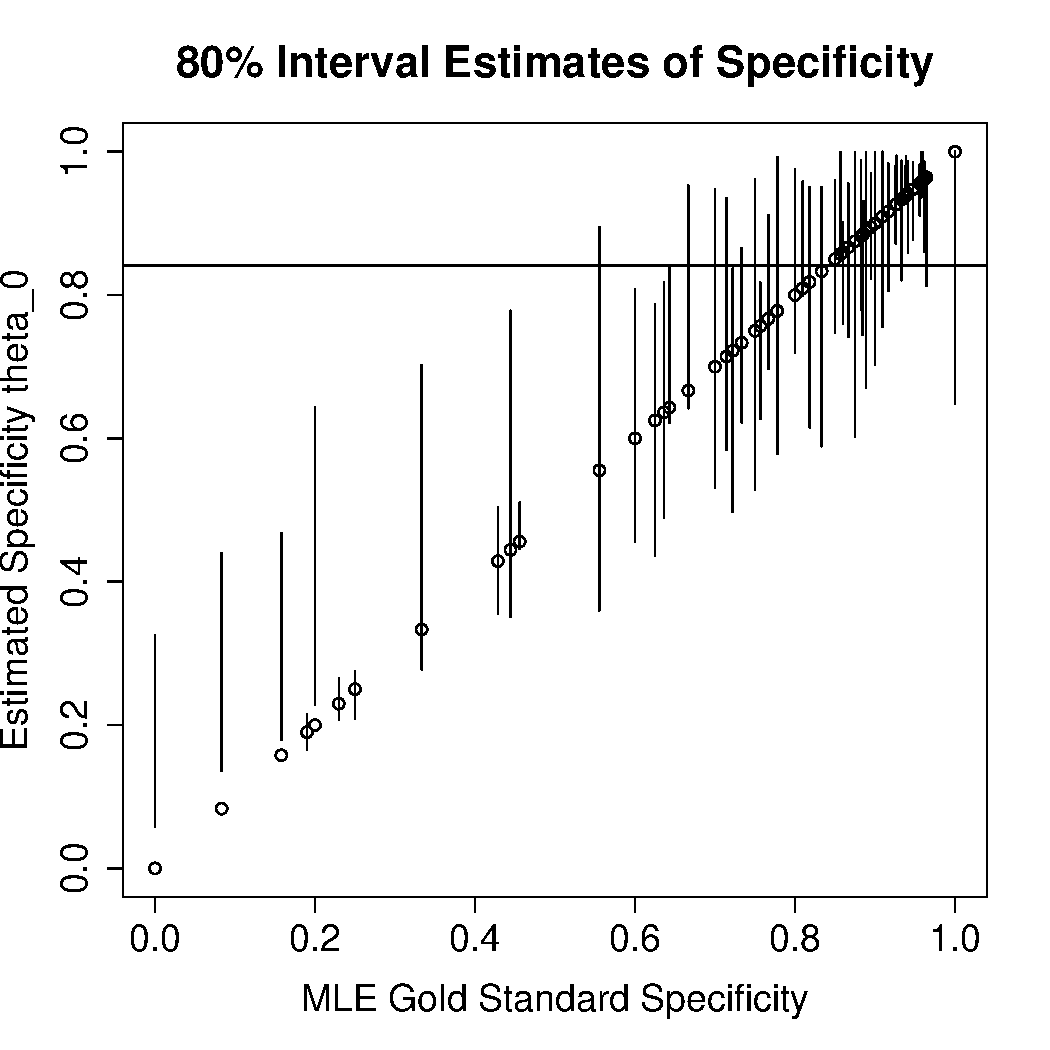
\includegraphics[width=0.4\textwidth]{pdf/dolores-beta-binomial-resid-spec.pdf}%
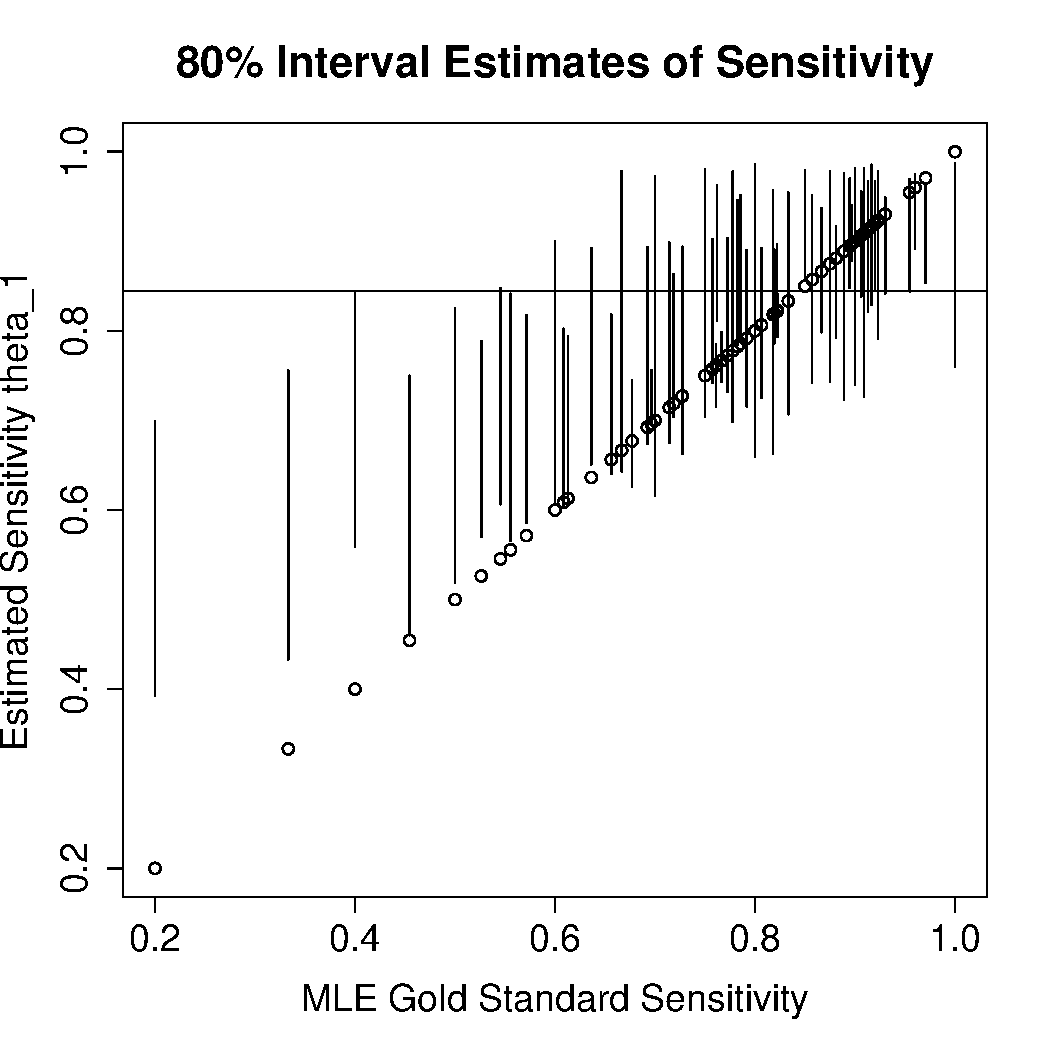
\includegraphics[width=0.4\textwidth]{pdf/dolores-beta-binomial-resid-sens.pdf}%
\end{center}
\mycaption{80\% posterior interval estimates of specificity and sensitivity parameters
$\theta_0$ and $\theta_1$ for annotators is plotted versus their
sample specificity and sensitivity evaluated against the RTE-1 test
data.  The circles indicate the specifity and sensitivity against the
gold standard, with vertical lines representing 80\% posterior
interval estimates.  The horizontal lines are at the beta prior's
estimated means for specificity and sensitivity,
$\alpha_0/(\alpha_0+\beta_0)$ and $\alpha_1/(\alpha_1+\beta_1)$.}
\label{dolores-sens-spec.fig}
\end{figure}
%
The figure illustrates the strong pull of the prior on the estimated
accuracies.  It also shows very wide posterior intervals around
annotators who annotated very few items (most annotators only did 20
items).  The 95\% posterior interval with median for the specificity
and sensitivity being $(.81,.84,.87)$ for
$\alpha_0/(\alpha_0+\beta_0)$ and $(.82,.84,.87)$ for
$\alpha_1/(\alpha_1 + \beta_1)$.  The prevalence of category 1
responses has posterior interval $(.45,.49,.52)$, which closely
matches the sample prevalence of 0.5 (400 positive, 400 negative cases
according to the gold standard).  The posterior intervals for the beta
prior scales for specificity and sensitivity are $(2.0, 2.8, 3.9)$ for
$\alpha_0 + \beta_0$ and $(6.9, 10.9, 17.6)$ for $\alpha_1 + \beta_1$.

\begin{figure}
\begin{center}
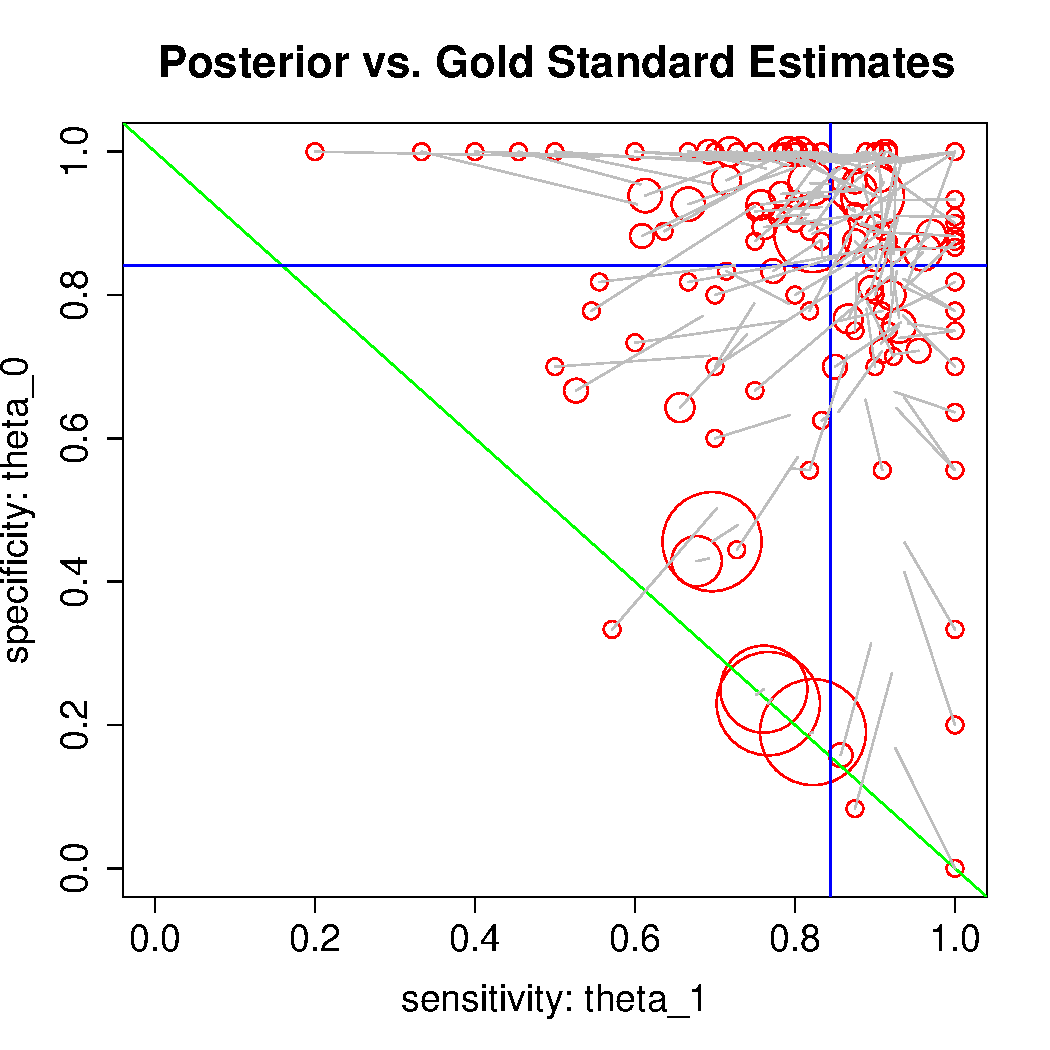
\includegraphics[width=0.4\textwidth]{pdf/dolores-rte-resids2D.pdf}%
\end{center}
\mycaption{Each circle represents a different annotator.  The circles
are centered on the empirical maximum likelihood estimate versus the
RTE-1 gold-standard.  The circles are sized proportionally to the number
of items annotated, which ranged from 20--800.  The gray lines run
from the circle centers to the estimates produced by the beta-binomial
by annotator model.  The horizontal and vertical blue lines are placed
at the beta prior means, $\alpha_0/(\alpha_0+\beta_0)$ and
$\alpha_1/(\alpha_1+\beta_1)$.  The diagonal green line indicates
chance performance, with position on the green line corresponding to
bias, with the edges indicating all 1 or all 0 annotations.}%
\label{dolores-rte-resids2D.fig}
\end{figure}
%
We present a different plot of the residuals versus the gold standard
in Figure~\ref{dolores-rte-resids2D.fig}.  This diagram makes it clear
that annotators not only vary with respect to their bias towards
sensitivity or specificity, but that they also vary in accuracy.

For this task, there were a large number of annotators who labeled the
data randomly.  The diagonal green line in
Figure~\ref{dolores-rte-resids2D.fig} indicates random performance,
with the ratio of 1 to 0 responses indicated by the position along the
line.  This represents a substantial amount of noise relative to
reliable data.  By jointly estimating annotator accuracies, the model
is able to automatically filter out the effect of the noise.  Suppose
we were to remove all annotators with an estimated sensitivity or
specificity below 50\% and refit the model.  The results are dispalyed
in Figure~\ref{dolores-rte-resids2D-pruned.fig}.
%
\begin{figure}
\begin{center}
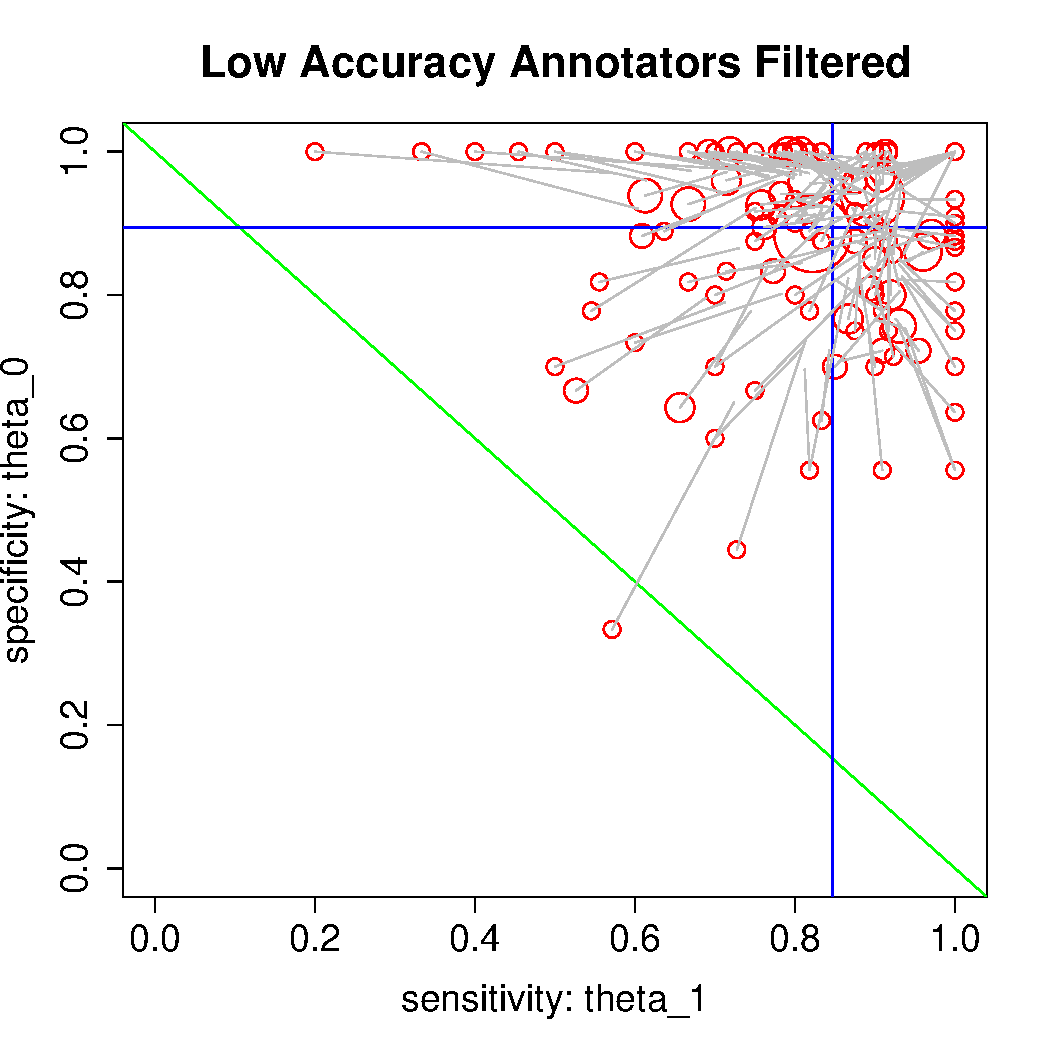
\includegraphics[width=0.4\textwidth]{pdf/dolores-rte-resids2D-pruned.pdf}%
\end{center}
\mycaption{The same type of diagram as Figure~\ref{dolores-rte-resids2D.fig}, after
removing annotators with sensitivity or specificity estimated to be below 50\% and
refitting the model.  The mean sensitivity and specificity as indicated
by the blue lines have gone up.}%
\label{dolores-rte-resids2D-pruned.fig}
\end{figure}
%
As can be seen in Figure~\ref{dolores-rte-resids2D.fig}, the
low-accuracy annotators account for a disproportionate number of
annotations per annotator.  That is, the noise generators were
prolific.  After filtering them out, only 4880/8000 = 61\% of the
annotations were left, making estimation that much more difficult due
to the sparsity of the reliable data points.  Filtering the
low-accuracy annotators proportionally improves the claims made by
Snow et al.~about the number of mechanical Turk annotators required to
reprodduce the accuracy of an ``expert'' annotator.

The very worst annotator, as measured against the gold standard by
being below chance performance, is not filtered, because the prior
exerts a strong pull on annotators who only labeled 20 examples.  A
better pruning strategy would be to remove annotators who did not
perform sufficiently better than chance, for instance, as calculated
by a $\kappa$ statistic versus the gold standard.  In this case, the
results are the same except for the few annotators at the far margins
of the border who perform better than chance with a large bias.
Depending on where the boundary is set around chance performance, this
strategy could have filtered out some more of the poorer performers.

The posterior 95\% intervals and mean for prevalence $\pi$ with
low-accuracy annotators filtered out are $(.45,.49,.53)$.  Posterior
intervals for specificity and sensitivity go up to $(.88,.90,.92)$ and
$(.82,.85,.87)$ respectively, indicating quite good agreement by the
mechanical Turk annotators with the inferred gold standard.  The
posterior estimates for the scales for specificity and sensitivity are
$(6,9,16)$ for $\alpha_0 + \beta_0$ and $(7,12,22)$ for $\alpha_1 +
\beta_1$, indicating slightly less variability in sensitivity than
specificity.  Removing noisy annotators substantially reduces the
estimates of variability and increases the estimates of accuracy,
especially for sensitivity.

Suppose we have two independent annotators with specificity of .9 and
sensitivity of .85 and a problem with a prevalence of 0.5.  We expect
inter-annotator agreement to be:
\[
0.5 \times (0.9^2 + 0.1^2) + 0.5 \times (0.85^2 + 0.15^2)
= 0.78
\]
corresponding to $\kappa=.56$ (see below for a definition of
$\kappa$).  This is generally considered too low to create a reliable
gold standard, but we have shown that by aggregating over a large
number of unreliable annotators, we can achieve a gold standard at
least as well annotated as one annotated by two or three experts.

We plot how well our model-based estimates fare against a simple voted
estimated versus the gold standard.  Both results are plotted
in Figure~\ref{dolores-cat-resids.fig}.
%
\begin{figure}
\begin{center}
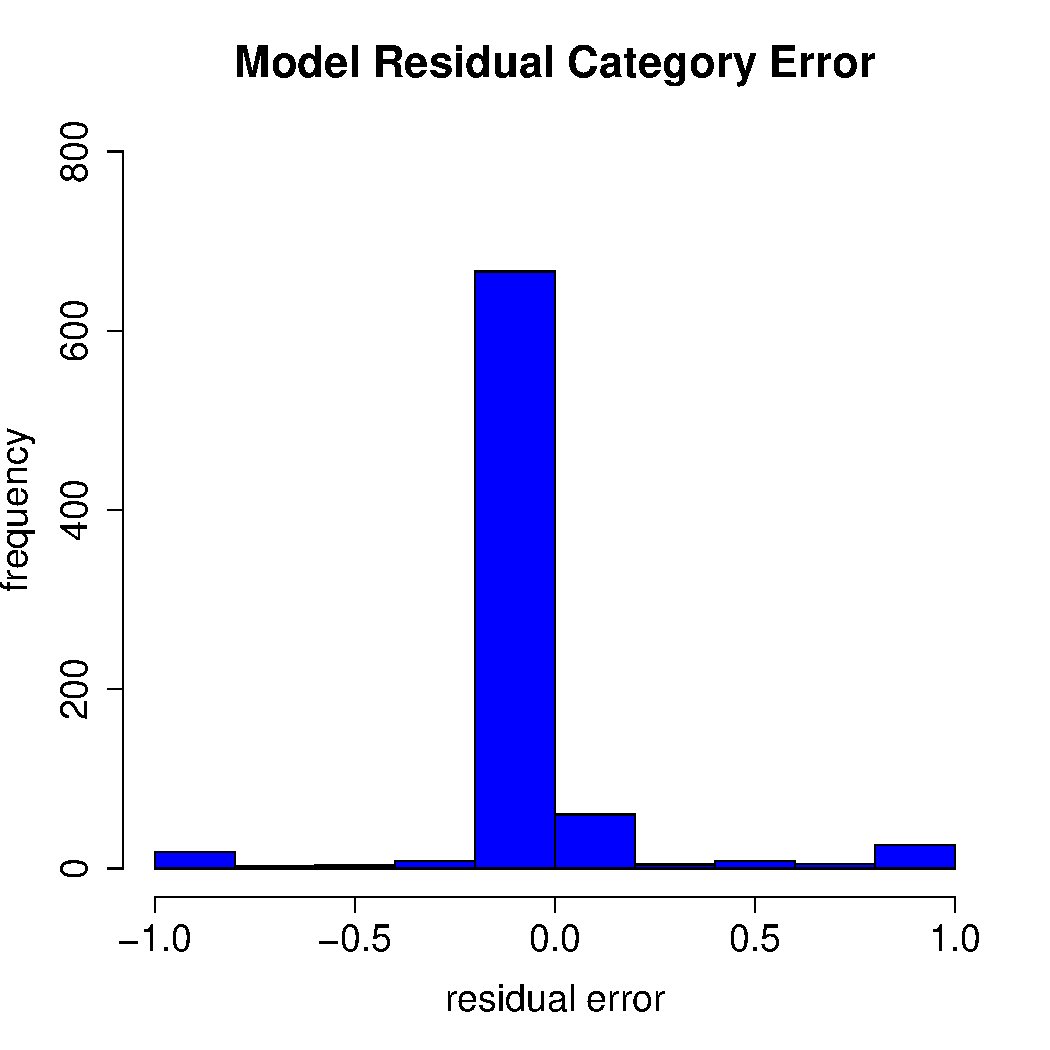
\includegraphics[width=0.4\textwidth]{pdf/dolores-cat-resids-model.pdf}%
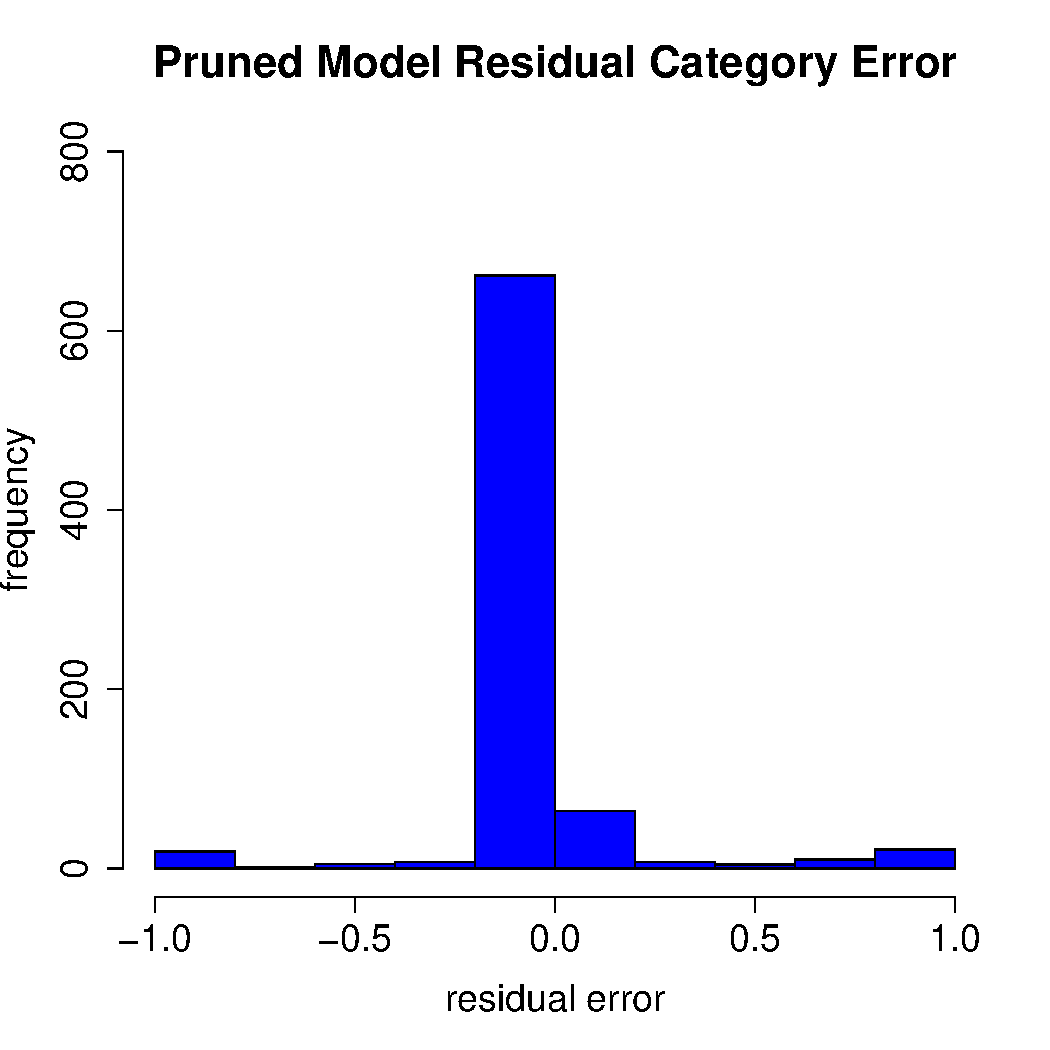
\includegraphics[width=0.4\textwidth]{pdf/dolores-cat-resids-model-pruned.pdf}%
\\[4pt]
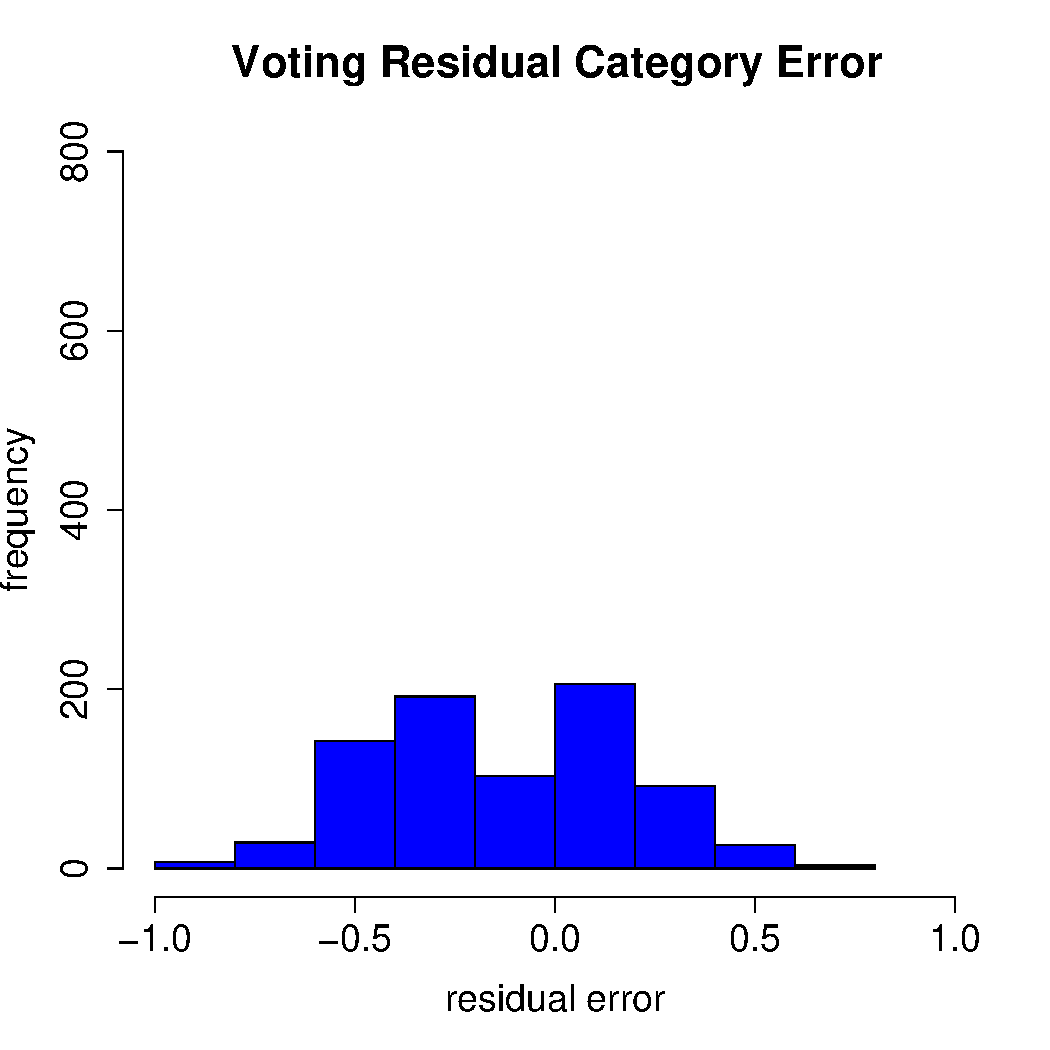
\includegraphics[width=0.4\textwidth]{pdf/dolores-cat-resids-voted.pdf}%
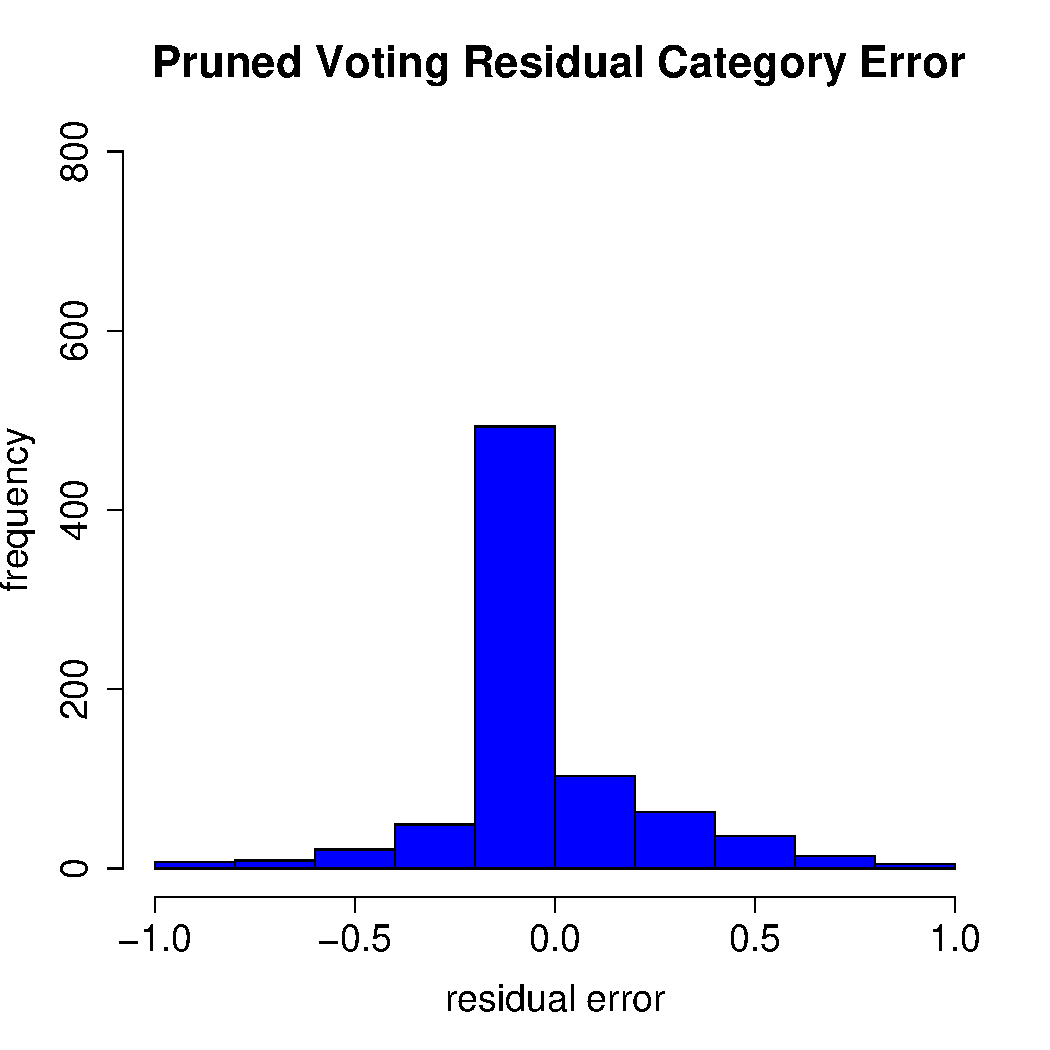
\includegraphics[width=0.4\textwidth]{pdf/dolores-cat-resids-voted-pruned.pdf}%
\end{center}
\mycaption{Residual category errors for the model posterior category
estimate before and after pruning low-accuracy annotators versus the
gold standard and simple voting versus the gold standard with no
pruning of low-accuracy annotators.}%
\label{dolores-cat-resids.fig}
\end{figure}
%
The residuals for the model-based estimates, both before and after pruning
low-accuracy annotators, are much sharper.  The
model-based estimate for the category of item $i$ is the mean of the
posterior samples $c_i^{(n)}$.  The voted estimate is the mean of the
estimates $xx_k$ such that $ii_k=1$; in all cases there are ten such
$xx_k$ because of the data design of ten annotators per item.

There were 50 cases where voting produced residual error greater than
0.5 and 65 cases which were tied.  If ties are broken by coin
flipping, that's an expected number of errors of $50+65/2 = 82.5$, for
an expected accuracy of .897.  The model-based estimate before pruning
low-accuracy annotators has 58 errors, for an accuracy of .928.  After
pruning low-accuracy annotators (recall that this is without recourse
to the gold-standard), the model-based estimate has 55 errors versus
the gold standard, for an estimated accuracy of .931.  Simple voting
after the low-accuracy annotators are removed (based on initial model
fit) leads to 49 errors and 22 ties, for an expected number of errors
of 59.5 and an expected accuracy of .925.

Snow et al.\ showed similar results with a point estimate of annotator
sensitivity and specificity using Laplace smoothing (that is, a maximum
a posterior binomial estimate with a $\mbox{\sf Beta}(2,2)$ prior).

We further estimated a non-hierarchical version of the model with a
$\mbox{\sf Beta}(1,1)$ prior to simulate maximum likelihood
inference; that model had one less error than the hierarchical model.
As usual, the hierarchical model exerts a degree of smoothing that
results in a slightly less tight fit to the training data, but
hopefully a better estimate of underlying ability and thus more
generalizability to future data because of less overfitting to the
training data.

For some annotators, there are only 20 items from which to estimate
their accuracy. The Bayesian aspect of the model is reflected in
the wide posterior interval for sensitivity and specificity estimates.
The hierarchical aspect of the model is evidenced by pulling
estimates of ability based on low counts closer to the mean.

We also estimated the logistic model with item and annotator effects.
The chains converged quickly, with all $\hat{R}$ values near 1.  The
95\% posterior interval and median for the prevalence parameter $\pi$
is $(.46,.49,.52)$, matching the beta-binomial by annotator model
estimates almost exactly.  The hierarchical parameters in this case
are the means and variances of the item and annotator coefficients
$\gamma$ and $\delta$.  The posterior interval and mean for $\mu_0$ is
$(2.0,2.3,2.6)$ and for $\mu_1$ is $(1.7,1.9,2.2)$. These values are
on the logit scale; converting to the probability scale we have
posterior intervals for $\mbox{\rm logit}^{-1}(\mu_0)$ of
$(.88,.91,.93)$ and for $\mbox{\rm logit}^{-1}(\mu_1)$ of
$(.85,.87,.90)$.  These are also very close to the estimates in the
beta-binomial by annotator model.  The posterior intervals for prior
deviation for $\sigma_0$ are $(1.1,1.3,1.5)$ and for $\sigma_1$ are
$(.60,.82,1.06)$.  The item parameters have a prior mean centered at
0, with posterior quantiles for deviation for $\rho_0$ of
$(.05,.24,.36)$ and for $\rho_1$ of $(.21,.31,.39)$, which in turn
exert a strong pull toward 0 for item difficulty parameters $\delta$.
As a result, the residuals and other estimates look very similar to
those of the beta-binomial by annotator model, including exactly 55
items with residual errors for category assignment greater than or
equal to 0.5.

The model-based posteriors are almost certainly too sharp due to the
unwarranted uniform difficulty assumption of the beta-binomial by
annotator model.

Annotating a corpus could proceed by continuing to supply annotators
until posterior intervals were tight around 0 or 1.  Under this
approach, some of the categories are still suspect.  There are 109
items whose posterior category mean is in (.01,.99), indicating
uncertainty in the model.  Of the remaining 691 items with mean
category posterior below .01 or above .99, 18 have category
assignments that do not match the gold standard.

Closer inspection of the residual errors shows some very problematic
cases.  Consider this case:
%
\begin{quote}
{\it Text:}
Seiler was reported missing March 27 and was found four days later in a
marsh near her campus apartment.
\\[4pt]
{\it Hypothesis:} Abducted Audrey Seiler found four days after missing.
\end{quote}
%
The mechanical Turk annotators were sure this was a negative instance,
but the gold standard marked it as positive.

Examples like this bring up the problem of what it means to probably
entail something, where the following was marked as false in the gold
standard data (as it should be):
%
\begin{quote}
{\it Text:} Kennedy had just won California's Democratic presidential primary when Sirhan shot him in Los Angeles on June 5, 1968.
\\[4pt]
{\it Hypothesis:} Sirhan killed Kennedy.
\end{quote}
%
But what about world knowledge?  We know Sirhan in fact did kill
Kennedy by shooting him.

More subtle cases are on the not-quite inferred boundary, where the
following was marked true, though it didn't say they'd remove De Klerk's
name, just the accusatory paragraphs:
%
\begin{quote}
{\it Text:} The Supreme Court was due to decide today, Wednesday, on the appeal filed by De Klerk for the purpose of omitting the accusatory paragraphs against him in the report, especially the paragraphs on his responsibility for bloody attacks that were carried out in the eighties against anti-apartheid organizations.
\\[4pt]
{\it Hypothesis:} De Klerk awaits the Supreme court decision regarding the omission of his name in the incriminating report.
\end{quote}
%

On the other hand, the following example was coded as true in
the gold standard:
%
\begin{quote}
{\it Text:} Google files for its long awaited IPO.
\\[4pt]
{\it Hypothesis:} Google goes public.
\end{quote}
%
even though filing for an IPO isn't the same as going public:

Here's an item marked true in the gold standard that's clearly false
according to the instructions:
%
\begin{quote}
{\it Text:} Sonia Gandhi can be defeated in the next elections in India if between now and 2009, BJP can make Rural India Shine, if it can make every young man have a job that he can be proud of.
\\[4pt]
{\it Hypothesis:} Next elections in India will take place in 2009.
\end{quote}
%
The phrase ``between now and 2009'' doesn't mean 2009; the annotation
of the gold standard was done several years before 2008 and the mechanical
Turk annotations in 2008.  It's possible for this kind of data for
annotations to change, because world knowledge, which is part of the task,
changes over time.

Consider this example, which requires world knowledge:
%
\begin{quote}
{\it Text:} Microsoft was established in Italy in 1985.
\\[4pt]
{\it Hypothesis:} Microsoft was established in 1985.
\end{quote}
%
The gold standard marked this inference as false, but the mechanical
Turk annotators marked it true.  In a literal sense, the mechanical
Turk annotators are right if the prepositional phrase ``in Italy''
is taken as restrictive.  It's only through world knowledge about
Microsoft that the gold standard annotation of false is possible.

There are two morals to this story. First, you should always look at
your data! Over half of the residual disagreements between the Turker
annotations and the gold standard were of this highly suspect nature
and some were just wrong. Second, we need to be very careful in
explaining and clarifying the tasks we're asking annotators to do. The
user interface component is very important.



\section{Bayesian Kappa Statistics}

For the models that estimate annotator sensitivity and specificity, we
can estimate pairwise $\kappa$ statistics through marginal posteriors.

For simplicity of notation in this section, we will assume a
complete-panel design in which every annotator labeled every example;
it is a straightforward exercise in subscripting to extend these ideas
to the missing annotation and replicated data situations.

The sample kappa statistic between two annotators $j$ and $j'$ over
a data matrix $x$ is defined by:
\[
\kappa_{j,j'}(x) = \frac{A_{j,j'}(x) - C_{j,j'}(x)}{1 - C_{j,j'}(x)}
\]
The value $A_{j,j'}$ is the percentage of items for which the
two annotators supplied the same label:
\[
A_{j,j'}(x) = \frac{\sum_i (x_{i,j} = x_{i,j'})}{I}
\]
The value $C_{j,j'}$ is the expected agreement by independent
generation of labels under a maximum likelihood estimate of an
estimator's marginal category distributions:
\[
E_{j,j'}(x) = \frac{n_{1,j}}{I} \frac{n_{1,j'}}{I}
            + \frac{n_{0,j}}{I} \frac{n_{0,j'}}{I}
= \frac{n_{1,j} n_{1,j'} + n_{0,j} n_{0,j'}}{I^2}
\]
The subscripted $n$ variables are counts of 1 or 0 labels by annotator $j$:
\[
n_{1,j} = \sum_i x_{i,j} \ \ \ n_{0,j} = \sum_i (1 - x_{i,j})
\]

The predictive inference for the marginal density of $\kappa_{j,j'}$
given the data $x$ is:
\[
p(\kappa_{j,j'}|x) = \int_{\Theta} p(\kappa_{j,j'}|\theta) p(\theta|x) d\theta
\]
The integral averaging over $\theta$ is calculated by averaging over
the Gibbs samples $\theta^{(n)}$, which are drawn from the parameter
posterior $p(\theta|x)$.  To calculate $p(\kappa_{j,j'}|\theta)$, we
sample a fresh data set $y^{(n)}$ for each parameter sample
$\theta^{(n)}$ (as defined by the relevant model) and set:
\[
\kappa^{(n)} = \frac{A_{j,j'}(y^{(n)}) - E_{j,j'}(y^{(n)})}
                    {1 - E_{j,j'}(y^{(n)})}
\]
The set of these samples approximates the posterior marginal density
$p(\kappa|x)$.

In the beta-binomial by annotator model, $\kappa$ may be more
easily estimated through the prevalence estimate and the
estimates of annotator sensitivity and specificity:
%
\begin{eqnarray*}
E_{\pi,\theta_0,\theta_1}(\kappa_{j,j'}) & = &
\pi (\theta_{1,j} \theta_{1,j'} + (1 - \theta_{1,j})(1 - \theta_{1,j'})) \\[4pt]
& + & (1 - \pi) (\theta_{0,j} \theta_{0,j'} + (1 - \theta_{0,j})(1 - \theta_{0,j'}))
\end{eqnarray*}
%
The $(1-\theta)$ terms in the expectation represent the case where the
annotators agree by both making the same mistake.


\section{Corpus Adjudication, Coding Standard Development, and Annotator Evaluation}

The models we present in this paper have an obvious application in
corpus development.  We suggest a methodology in which items are first
presented to a minimum number of annotators and then to more
annotators as needed to infer the item's category or conclude the item
is difficult.

Difficult items have a role in defining the coding standard, as they
may point out boundary conditions or places where the original coding
standard was not clear.  They may also point out genuinely borderline
cases, which we recommend leaving in the corpus with their associated
posterior uncertainty.  That is, we believe a model should not be too
confident about such uncertain examples.

Our models may also be used to evaluate annotators.  The models
uncover bias toward 0 or 1 categories, as well as finding errors and
general trends in accuracy.  In the mechanical Turk setting, this can
be used to reject annotators or more highly compensate accurate ones.





\section{Probabilistic Supervision and Evaluation}

We can carry the Bayesian approach to category estimtaion straight
through classifier training and evaluation.  We can even use multiple
imputation techniques directly to train any old classifier in
a Bayesian fashion.

For training, we simply generate a number of Gibbs samples $c^{(n)}$
over complete category assignments to all items.  For instance, if we
take $N=100$ samples, we would have a training set 100 times as large
as originally.  Simple classifiers such as naive Bayes have sufficient
statistics which amount to counts for the category assignments and
items, which can greatly accelerate training.

Discriminative classifiers such as support vector machines,
perceptrons or logistic regression can very efficiently handle large
numbers of training items by means of the stochastic gradient descent
optimization algorithm which may be used for training (see Carpenter
2008).  With stochastic gradient descent, training events for epochs
can simply draw category assignments directly from the Gibbs samples
$c^{(n)}$ from the posterior.

Probabilistic evaluation may also be carried out in a Bayesian fashion
through sampling.  That is, the test set rather than consisting of
a single gold standard would consist of a number of samples from
the posterior category assginment.

Although we do not have the data to evaluate these methods, we believe
they will result in classifiers that are more robust in that they
learn not only the difference between items that should be in category
0 or 1, but they also learn not to be too confident at the boundaries.



\section{Previous Work}

Most of the work on models like these were carried out in the
epidemiology literature and the educational testing literature, with
only a little crossover to machine learning and natural language
processing.

Dawid and Skene (1979) introduced a multinomial classification model
in which each annotator's response varies by category, thus
generalizing the notion of sensitivity and specificity.  They assumed
conditional independence given true (latent) category and attempt to
find maximum likelihood point estimates using expectation maximization
(EM).

Hui and Walter (1980) introduced an a binomial model similar to Dawid
and Skene's multinomial and consider the identifiability conditions
for maximum likelihood estimators of prevalence, sensitivity and
specificity.

Lord (1980) and Rasch (1980) independently developed the item-response
model for educational testing applications.  The items are students
and the diagnoistic tests are true/false questions.  The general forms
of these models include offsets for minimum accuracy (presumably due
to guessing) and for discriminativeness of the item to model how
sharply it separates students that should pass or fail.  Item-response
models are almost always estimated with a known gold standard.

Dillon and Mulani(1984) introduce a latent class multinomial
categorical model to asses inter-annotator agreement.  They estimate
error rates (not broken into sensitivity and specificity) for the case
where all annotators have equal errors or where each has their own
error rate.  They provide maximum likelihood estimates using EM and
estimate goodness of fit using $\chi^2$ statistics on the marginal
empirical counts of annotations.

Vacek (1985) showed that Hui and Walter's estimates are biased if the
conditional independence assumption that errors are independent given
true category is violated.

Torrance-Rynard and Walter~(1997) provide an extensive simulation
analysis of the biases that arise from assuming conditional
independence of tests in latent class models when the tests are
actually dependent.

Espeland and Handelman (1989) introduce latent classes for items that
are unambiguously positive or negative in the sense that all tests are
expected to return the same result.  These models are able to account
for the number of all-0 and all-1 outcomes, which is almost always
higher than expected under the assumption of conditional independence.
This model is related to so-called ``zero-inflated'' Poisson models of
counts, which models the probability of zero counts separately from
non-zero counts.

Joseph, Gyorkos and Coupal (1995) introduce a binomial model for
sensitivity and specificity with independent beta priors.  They
estimate these priors using moment matching from a collection of prior
estimates by clinicians about their particular tests.  With only two
annotators, the priors exert a strong influence on the posterior
estimates of annotator sensitivity and specificity.  They use a
collapsed Gibbs sampler which integrates out the individual item
parameters, allowing direct updates for their parameters of interest.

Uebersax and Grove (1993) apply a variant of the item-response model
to the problem of agreement analysis in an ordinal response setting
when the gold standard is not known.  They assume latent traits for
items generated by binary normal mixtures.  For example, antibody
levels might be represented by one normal distribution for healthy
individuals and another normal distribution for infected individuals,
thus representing the population as a mixture of the two distributions
weighted by prevalence of infection.  Uebersax and Grove also
introduce a latent trait for annotator bias, acting much like the
ability parameter in the item-response model.  Bias is a weaker
measure of the difference between sensitivity and specificity which
assumes the two are related through bias.  Uebersax and Grove also
discuss a latent item-difficulty parameter, including a multiplicative
factor per rater, thus making it a measure of rater variance.  They
also discuss missing data, as well as replicated data (multiple
annotations of a single item by a coder).

Qu, Tan and Kutner~(1996) applied a generalized linear model, using
the probit link function, fitting a point estimate with expectation
maximization (EM).  They have parameters for annotator sensitivity and
specificity as well as item difficulty, with an additional
discriminative parameter for the diagnostic tests, which is similar to
the item discrimativeness parameter in the general item-response
model.  Their item difficulty parameters are set by hand to only
involve subsets of annotators, so that related diagnostics would have
correlated performance.

Dendukuri and Joseph~(2001) apply Bayesian inference to Qu, Tan and
Kutner's model, fixing priors by interviewing human experts.

Mendoza-Blanco, Tu and Iyengar (1996) apply Bayesian inference to include the
uncertainty in sensitivity and specificity estimates in estimating
prevalence in a model like Dawid and Skene's.

Tu, Kowalski and Jia (1999) extend Mendoza-Blanco, Tu and Iyengar's model to handle
item-level predictors in HIV diagnosis, such as age and number of
unprotected sexual context.  Sensitivity and specificity are well
constrained by beta priors estimated by experts.  Estimation is
carried out by Gibbs sampling.

Albert, McShane and Shih (2001) extend Espeland and Handelman's (1989) models
with item-level predictors such as subject age and disease severity.
They use the bootstrap over maximum likelihood estimates in order to
estimate standard errors.  They also extend Vacek's (1985)
demonstrations by considering more general failure of independence and
model structure, evaluating the simple binomial, the logistic random
effects model, and the mixture of easy/hard cases against data
generated by the mixture or logistic models.

Albert and Dodd~(2004) evaluate the bias induced in prevalence,
sensitivity and specificity estimates by choosing the wrong model.
They fit a binomial mixture model with easy/regular cases, a
beta-binomial model which shows item effects but treats annotators
homogeneously, as well as Qu, Tan and Kutner's logistic model with item effects
and annotator discriminativeness parameters.  They showed that all
three models predicted the histograms of counts by voting, and the
binomial mixture and ``random effects'' models also fit the individual
outcomes well.

Walter~(1999) considers the natural epidemiological case where only
positive test cases are confirmed.  That is, if a diagnostic test was
positive for a disease, a more expensive and/or more dangerous test
was used to determine a gold standard.  This leaves missing data for
the cases where the tests are negative.

Merwe and Maritz (2002) generalizes Walter's (1999) models to interactions
among annotators' responses.

Basu, Banerjee and Sen~(2000) develop a Bayesian estimate of the kappa
statistic (chance adjusted inter-rater agreement) by supplying a beta
prior for binomial responses and then reasoning about values of kappa
derived in the posterior beta distribution.

Broemeling~(2001) develops a Bayesian analysis of agreement among
annotators for low-count psychiatric diagnosis data, providing a
Dirichlet prior for the multinomial rating data, sampling from the
posterior Dirichlet to derive posterior intervals for agreement
numbers.

Smyth, Fayyad, Burl, Perona and Baldi (1994) use Dawid and Skene's
model to estimate gold standards from annotations by four geologists
of radar images collected by the Magellan spacecraft of Venus for
volcaons on an ordinal 1 to 5 scale, which could then be projected
onto a 0/1 scale for no-volcano/volcano.

Smyth (1995) discusses probabilistic supervision under exactly the
same kind of situation as we are discussing and shows it can work well
for simulated data.

Bruce and Wiebe (1999) apply Dawid and Skene's (1979) model estimated
by maximum likelihood to the problem of annotating text as to whether
it's subjective or objective.

Klebanov, Biegman and Diermeier (2008) apply the idea of
a mixture of trivial and regular cases in roughly the same
way as suggested  by Albert, McShane and Shih (2001).  They explicitly
state their goal is filtering out examples to produce a reliable
gold standard.

Sheng, Provost and Ipeirotis (2008) also study human annotators for
classification problems, analyzing agreement with simple uniformity
and independence assumptions, with a goal of directing active assignment
of annotators to new items or to relabeling existing items.

Snow, O'Connor, Jurafsky and Ng (2008) consider how many noisy
annotators would be required to recreate a ``gold standard'',
analyzing five natural language corpora with analyses generated from
Amazon's Mechanical Turk service.  We described their experiments on
the textual entailment challenge data in which they estimated
annotator sensitivity and specificity versus gold standard data using
Laplace smoothing, and used the resulting estimates to derive their
own reference annotations.

\subsection{What's New}

An innovation we have not seen in the epidemiology literature but we
consider here is the estimation of the group-level priors, such as
beta priors for sensitivity and specificity.  Our intended application
is somewhat different than epidemiology in that we can sometimes
gather large numbers of (conditionally) independent annotators,
whereas epidemiological applications are often limited to a few
diagnostic tests.

We also consider the common situation for data annotation in which
data is missing at random.  In all of the epidemiological studies we
cited, all tests were applied to all items.

We focus on the problem of arriving at an item-level gold standard,
whereas the epidemiology literature is much more concerned with
evaluating population prevalence and the sensitivity and specificity
of available diagnostic tests.

Unlike many of the epidemiology papers, we perform Bayesian inference
with Gibbs sampling.  As the models are introduced, they will be
evaluated with simulations to ensure that they can be fit from
appropriately distributed data.


\subsection{What's Next}

Now that we have established that our posterior estimtaes can be
reliable with noisily annotated data, it remains to be seen if we can
make use of this data in training and evaluating probabilistic
classifiers.  We are presently looking at collecting large amounts
of named-entity annotations from the mechanical Turk with an eye
toward recreating the MUC-6 data and evaluating it before creating
new data sets in multiple languages.

We also wish to work on one extension and one expansion and one
simplification of the regression-style models.  For extension, we want
to consider difficulty parameters as employed by the item-response
models, and the logistic epidemiology models.  For simplification, we
want to explore Uebersax and Grove's (1993) mixture modeling approach,
which estimates annotator bias and accuracy directly against an
underlying latent trait level, rather than estimating sensitivity and
specificty.  

If someone could send us conference review data of a large enough
size, it would be nice to apply these models to paper selection.  The
binary categories are accept/reject, and the usual 1-5 scale may be
rendered as a latent trait level.  Again, Uebersax and Grove's (1993)
model is promising for that problem.

Another area of application would be in weighting committee-based
classifiers in cases where there is no training data to calibrate
their accuracies.  The posterior model-based predictions of our
annotation models could be easily used to combine the votes of
automatic systems in classification problems.

Finally, we would like to explore some multinomial and ordinal
classification problems.  In this setting, the binomial models are
easier to expand to multinomial problems and the logistic models
easier to expand to ordinal problems.



\section*{Acknowledgements}

We'd like to thank Rion Snow, Brendan O'Connor, Victor Sheng, Panos
Ipeirotis, and Foster Prevost for discussions relating to
classification data and inter-annotator agreement, and Yajima Masanao, Aleks Jakulin,
Jennifer Hill, and Andrew Gelman for help designing and fitting the
models.  Rather than claiming the mistakes are all mine, I can further
state that the statisticians did not like the binomial models, and as
for the logistic models, they were very skeptical about estimating
sensitivity and specificity parameters separately rather than
following Uebersax and Grove's (1993) approach.

The project described was supported by Grant Number R44 RR020259 from
the (U.S.) National Center For Research Resources. The content is solely the
responsibility of the authors and does not necessarily represent the
official views of the National Center for Research Resources or the
National Institutes of Health.

\section*{References}

\begin{enumerate}

\item
Agresti, Alan and Joseph B.~Lang. 1993.
Quasi-symmetric latent class models, with application to rater agreement.
{\it Biometrics} {\bf 49}(1):131--139.

\item
Albert, Paul~S.\ and Lori~E.~Dodd.  2004.  A cautionary note on the
robustness of latent class models for estimating diagnostic error
without a gold standard. {\it Biometrics} {\bf 60}(2):427--435.

\item
Albert, Paul S., Lisa M.~McShane, Joanna H.~Shih, and the
U.~S.~National Cancer Institute Bladder Tumor Marker Network.  2001.
Latent class modeling approaches for assessing diagnostic error
without a gold standard: with applications to p53 immunohistochemical
assyas in bladder tumors.  {\it Biometrics} {\bf 57}(2):610--619.

\item
Alvord, W.~G., J.~E.~Drummond, L.~O.~Arthur, J.~J.~Goedert,
P.H.~Levine, E.~L.~Murphy Jr., S.~H.~Weiss, and W.~A.~Blattner.  1988.
A method for predicting individual HIV infection status in the absence
of clinical informaiton.  {\it AIDS Research and Human Retroviruses}
{\bf 4}:295--304.

\item
Basu, Sanjib, Mousumi Banerjee, and Ananda Sen. 2000.
Bayesian inference for kappa from single and multiple studies.
{\it Biometrics} {\bf 56}(2):577--582.

\item
Boelaert, M., K.~Aoun, J.~Liinev, E.~Goetghebeur, and P.~van~der~Stuyft.
1999.  The potential of Latent Class Analysis in diagnostic test
validation for canine {\it Leishmania infantum} infection.
{\it Epidemiol. Infect.} {\bf 123}:499--506.

\item
Bruce, Rebecca F. and Janyce M. Wiebe.  1999.  Recognizing
subjectivity: a case study of manual tagging.  {\it Natural Language
Engineering} {\bf 1}(1):1--16.

\item
Carpenter, Bob. 2008. Lazy Sparse Stochastic Gradient Descent for
Regularized Multinomial Logistic Regression. Technical
Report. Alias-i.

\item
Center for Medicare and Medicaid Services and Department of Health and
Human Services.  2005.  ICD-9-CM Official Guidelines for Coding and
Reporting.
% Downloaded from {\tt\footnotesize http://www.cdc.gov/nchs/data/icd9/icdguide.pdf}.

\item
Dagan, Ido, Oren Glickman, and Bernardo Magnini. 2006. The PASCAL
Recognising Textual Entailment Challenge. In Qui�onero-Candela, J.;
I.~Dagan, B.~Magnini, and F.~d'Alch�-Buc (eds.) {\it Machine Learning
Challenges}. Lecture Notes in Computer Science , Vol. 3944, 177--190,
Springer.

\item
Dawid, A.~P. and A.~M.~Skene.  1979.  Maximum likelihood estimation of
observer error-rates using the EM algorithm.  {\it Applied Statistics}
{\bf 28}(1):20--28.

\item
Dendukuri, Nandini and Lawrence Joseph.  2001.  Bayesian approaches to
modeling the conditional dependence between multiple diagnostic tests.
{\it Biometrics} {\bf 57}(1):158--167.

\item
Dillon, W.~R.\ and N.~Mulani N. 1984. A probabilistic latent class model for
assessing inter-judge reliability. {\it Multivariate Behavioral Research}.
{\bf 19}:438-458.

\item
Espeland, M.~A. and S.~L.~Handelman.  1989.
Using latent class models to characterize and assess relative-error in
discrete measurements.  {\it Biometrics} {\bf 45}:587--599.

\item
Fanshawe, Thomas R., Andrew G.~Lynch, Ian O.~Ellis, Andrew R.~Green,
and Rudolf Hanka.  2008.  Assessing agreement between multiple raters with missing rating information, applied to breast cancer tumour grading.
{\it PLoS One} {\bf 3}(8), e2925.

\item
Gelman, Andrew, John B.~Carlin, Hal S.~Stern, and Donald B.~Rubin.
2003.  {\it Bayesian Data Analysis, 2nd Edition}.  Boca Raton,
Florida: Chapman Hall/CRC.

\item
Gelman, Andrew and Jennifer Hill. 2006.
{\it Data Analysis Using Regression and Multilevel/Hierarchical Models}.
Cambridge: Cambridge University Press.

\item
Gelman, Andrew and Donald B.~Rubin.
1992.
Inference from iterative simulation using multiple sequences.
{\it Statistical Science} {\bf 7}(4):457--472.

\item
Holmquist, N.~D., C.~A.~McMahan, and O.~D.~Williams.
Variability in classification of carcinoma in situ of the uterine cervix.
{\it Archives of Pathology} {\bf 84}:334--345.
1967.

\item
Hui, S.~L.\ and S.~D.~Walter.  1980.  Estimating the error rates of
diagnostic tests.  {\it Biometrics} {\bf 36}:167--171.

\item
Joseph, Lawrence, Theresa W.~Gyorkos, and Louis Coupal.  1995.
Bayesian estimation of disease prevalance and the parameters of
diagnostic tests in the absence of a gold standard.  {\it American
Journal of Epidemiology} {\bf 141}(3):263--272.

\item
Klebanov, Beata Beigman, Eyal Beigman, and Daniel Diermeier.  2008.
Analyzing disagreements.  In {\it Proceedings of the COLING 2008
Workshop on Human Judgments in Computational Linguistics}.
Manchester, U.K.

\item
Lord, Frederic~M.  1980.  {\it Applications of Item-Response Theory to
Practical Testing Problems}.  New Jersey: Lawrence Erlbaum Associates.

\item
Marsh, Elaine and Dennis Perzanowski.  1998.  MUC-7 Evaluation of IE
Technology: Overview of Results.  In {\it Proceedings of the Seventh
Message Understanding Conference}.

\item
Mendoza-Blanco, J. R., X.~M.~Tu, and S.~Iyengar. 1996. Bayesian
inference on prevalence using a missing- data approach with
simulation-based techniques: application to HIV screening. {\it Statistics
in Medicine} {\bf 15}:2161--2176.

\item
Merwe, Lize van der and J.~Stephan Maritz.  2002.  Estimating the
conditional false-positive rate for semi-latent data.  {\it
Epidemiology} {\bf 13}(4):424--430.

\item
Qu, Yinsheng, Ming Tan, and Michael H.~Kutner.  1996.  Random effects
models in latent class analysis for evaluating accuracy of diagnostic
tests. {\it Biometrics} {\bf 52}(3):797--810.

\item
R Core Development Team.  2008.  {\it R: A Language and Environment
for Statistical Computing}.  Vienna: R Foundation for Statistical
Computing.  ISBN 3-900051-07-0.


\item
Rasch, Georg. 1980.
{\it Probabilistic Models for Some Intelligence and Attainment Tests}.
Expanded Addition.
Chicago: University of Chicago Press.

\item
Reidsma, Dennis and Jean Carletta.  2008. Reliability measurement
without limits.  {\it Computational Linguistics}
{\bf 34}(3): 319--326.

\item
Santorini, Beatrice.  1990.  Part-of-speech tagging guidelines for the
Penn Treebank project (3rd Revision).  University of Pennsylvania
Department of Computer and Information Science Technical Report
No. MS-CIS-90-47.

\item
Sheng, Victor S., Foster Provost and Panagiotis G.~Ipeirotis.  2008.
Get another label? Improving data quality and data mining using
multiple, noisy labelers.  In {\it Proceedings of KDD '08}.

\item
Siegel, S. and N.~J.~Castellan, Jr. 1988. {\it Nonparametric Statistics
for the Behavioral Sciences}. McGraw-Hill.

\item
Smyth, Padhraic.
1995.
Learning with probabilistic supervision.
In Thomas Petsche, ed., {\it Computational Learning Theory and Natural
Learning Systems Volume III}.
Cambridge, MA. MIT Press.

\item
Snow, Rion, Brendan O'Connor, Daniel Jurafsky, and Andrew Y.~Ng. 2008.
Cheap and fast -- but is it good? Evaluating nonexpert annotations for
natural language tasks.  In {\it Proceedings of the 2008 Conference on
Empirical Methods in Natural Language Processing (EMNLP)}.  Honolulu,
Hawaii.

\item
Spiegelhalter, D.~J., A.~Thomas, and N.~G.~Best. 2008.
{\it WinBUGS Version 1.4.3 User Manual}.
MRC Biostatistics Unit.

\item
Sturtz, S., U. Ligges, and A. Gelman.  2005. R2WinBUGS: a package for
running WinBUGS from R.  {\it Journal of Statistical Software}. {\bf
12}(3), 1--16.

\item
Torrance-Rynard, Vicki L.\ and Stephen D.~Walter.
1997.
Effects of dependent errors in the assessment of diagnostic test performance.
{\it Statistics in Medicine} {\bf 16}:2157--2175.

\item
Tu, Xin M., Jeanne Kowalski, and Gang Jia.  1999.  Bayesian
analysis of prevalence with covariates using simulation-based
techniques: applications to HIV screening.  {\it Statistics in
Medicine} {\bf 18}(22):3059--3073.

\item
Uebersax, J.~S.\ and W.~M.~Grove.  1993.  A latent trait
finite mixture model for the analysis of rating agreement.  {\it
Biometrics} {\bf 49}(3):823--835.

\item
Vacek, P.~M. 1985.  The effect of conditional dependence on the
evaluation of diagnostic tests.  {\it Biometrics} {\bf 41}:959--968.

\item
Walter, S.~D. 1999.  Estimation of test sensitivity and
specificity when disease confirmation is limited to positive results.
{\it Epidemiology} {\bf 10}(1):67-72.

\item
Yang, Ilsoon and Mark P.~Becker. 1997.
Latent variable modeling of diagnostic accuracy.
{\it Biometrics} {\bf 53}(3):948--958.

\item
Yeh, Alexander, Alexander Morgan, Marc Colosimo, and Lynette Hirschman.
2005.
BioCreAtIvE task 1A: gene mention finding evaluation.
{\it BMC Bioinformatics} {\bf 6}(Suppl 1):S2.
{\tt doi:10.1186/1471-2105-6-S1-S2}.

\end{enumerate}



\end{document}

